\chapter{RESULTS AND ANALYSIS}


% (20\% of Report Length)

% a. Showcase the output at various intermediate stages of the project pipeline

% b. Use proper data visualizing techniques to present the output

% c. Figures and tables must be accompanied by an explanation

\section{User Interface}

\subsection{Mobile Application}

\textbf{Initial Login}\\
Initially, a user should provide National Identity Number along with the Mobile Number that is linked to their National Identity Card.
\begin{multicols}{2}
        \begin{figure}[H]
        \centering
        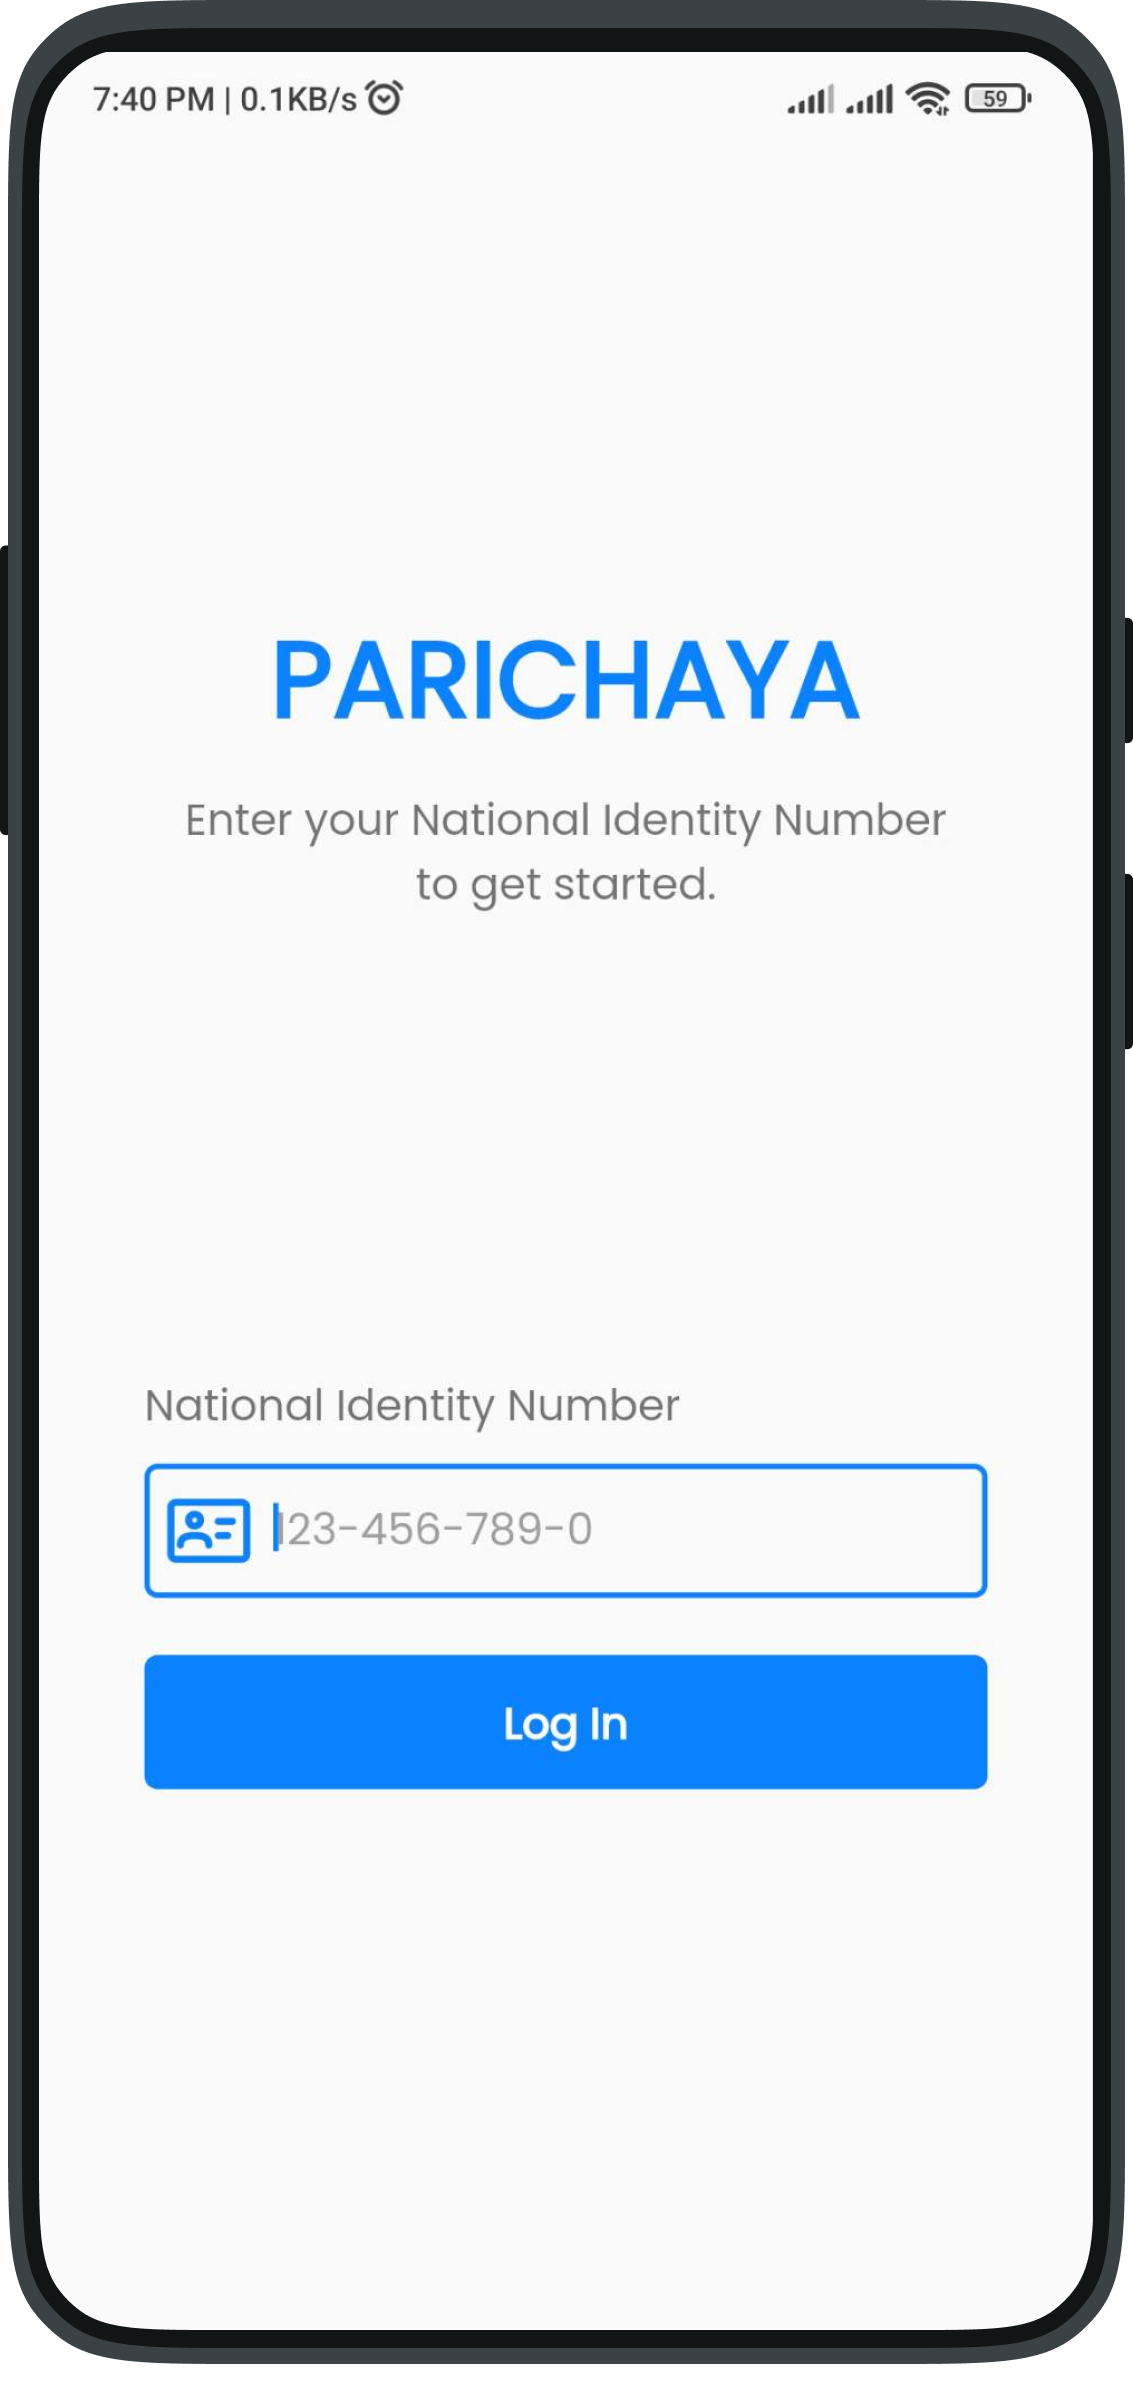
\includegraphics[width=0.6\linewidth]{images/results/mobile/LoginNIN.png}
        \caption[Enter NIN Screen]{Enter NIN Screen}
        \label{fig:LoginNIN.png}
        \end{figure}

      \begin{figure}[H]
            \centering
            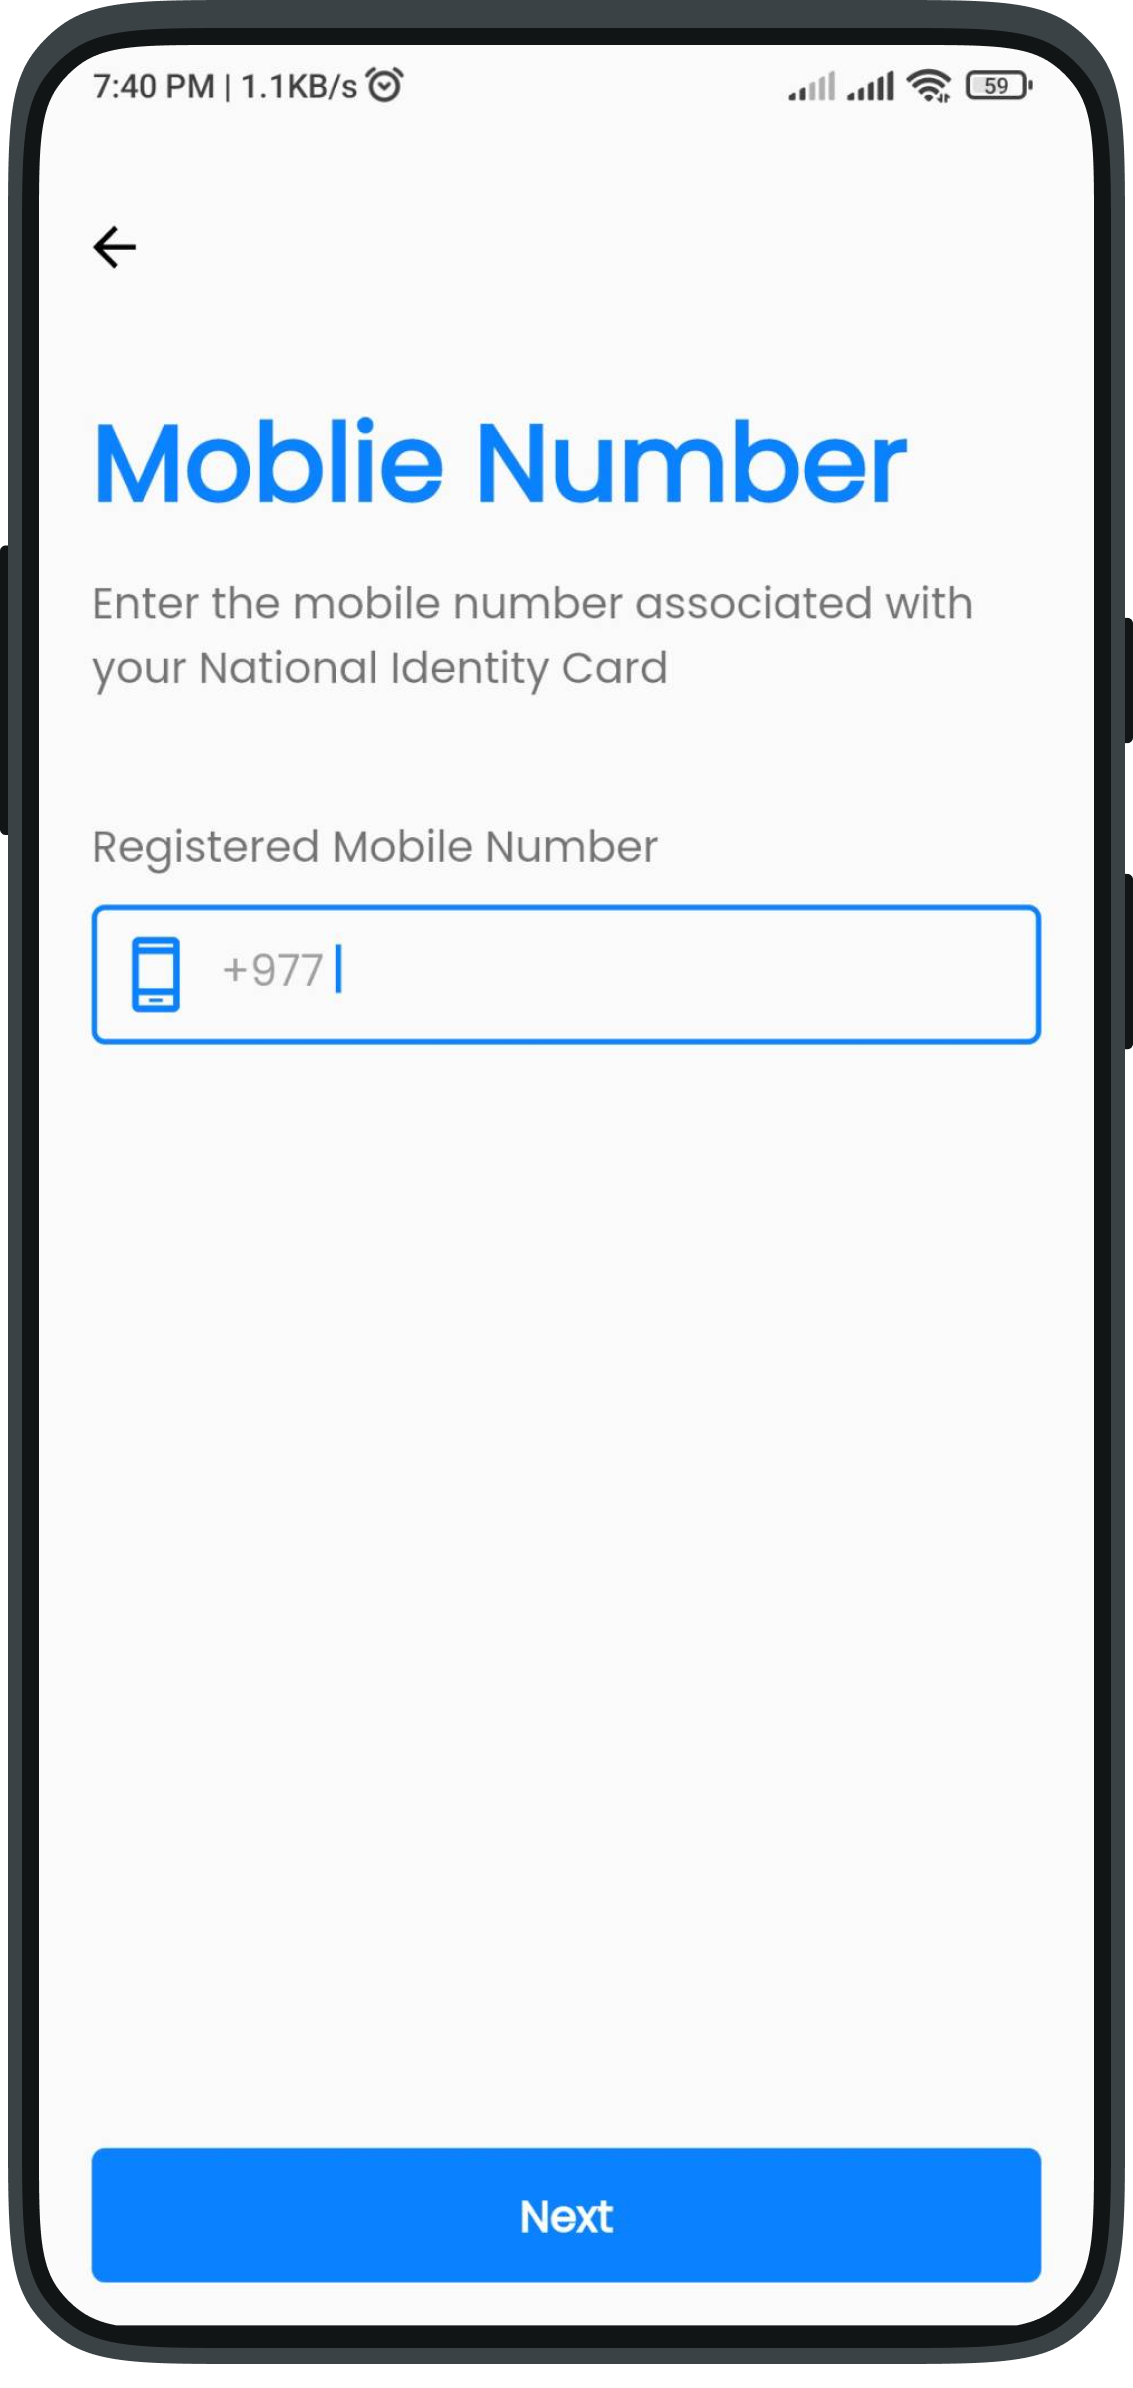
\includegraphics[width=0.6\linewidth]{images/results/mobile/MobileNumber.png}
            \caption[Enter Mobile Number Screen]{Enter Mobile Number Screen}
            \label{fig:MobileNumber.png}
            \end{figure}
\end{multicols}
\textbf{OTP Verification}\\
    If both of the number exist, an OTP is sent to the mobile number given by the user for verification. In case of an error, OTP can be resent to the user. 
    \newpage
    \begin{multicols}{2}
        \begin{figure}[H]
        \centering
        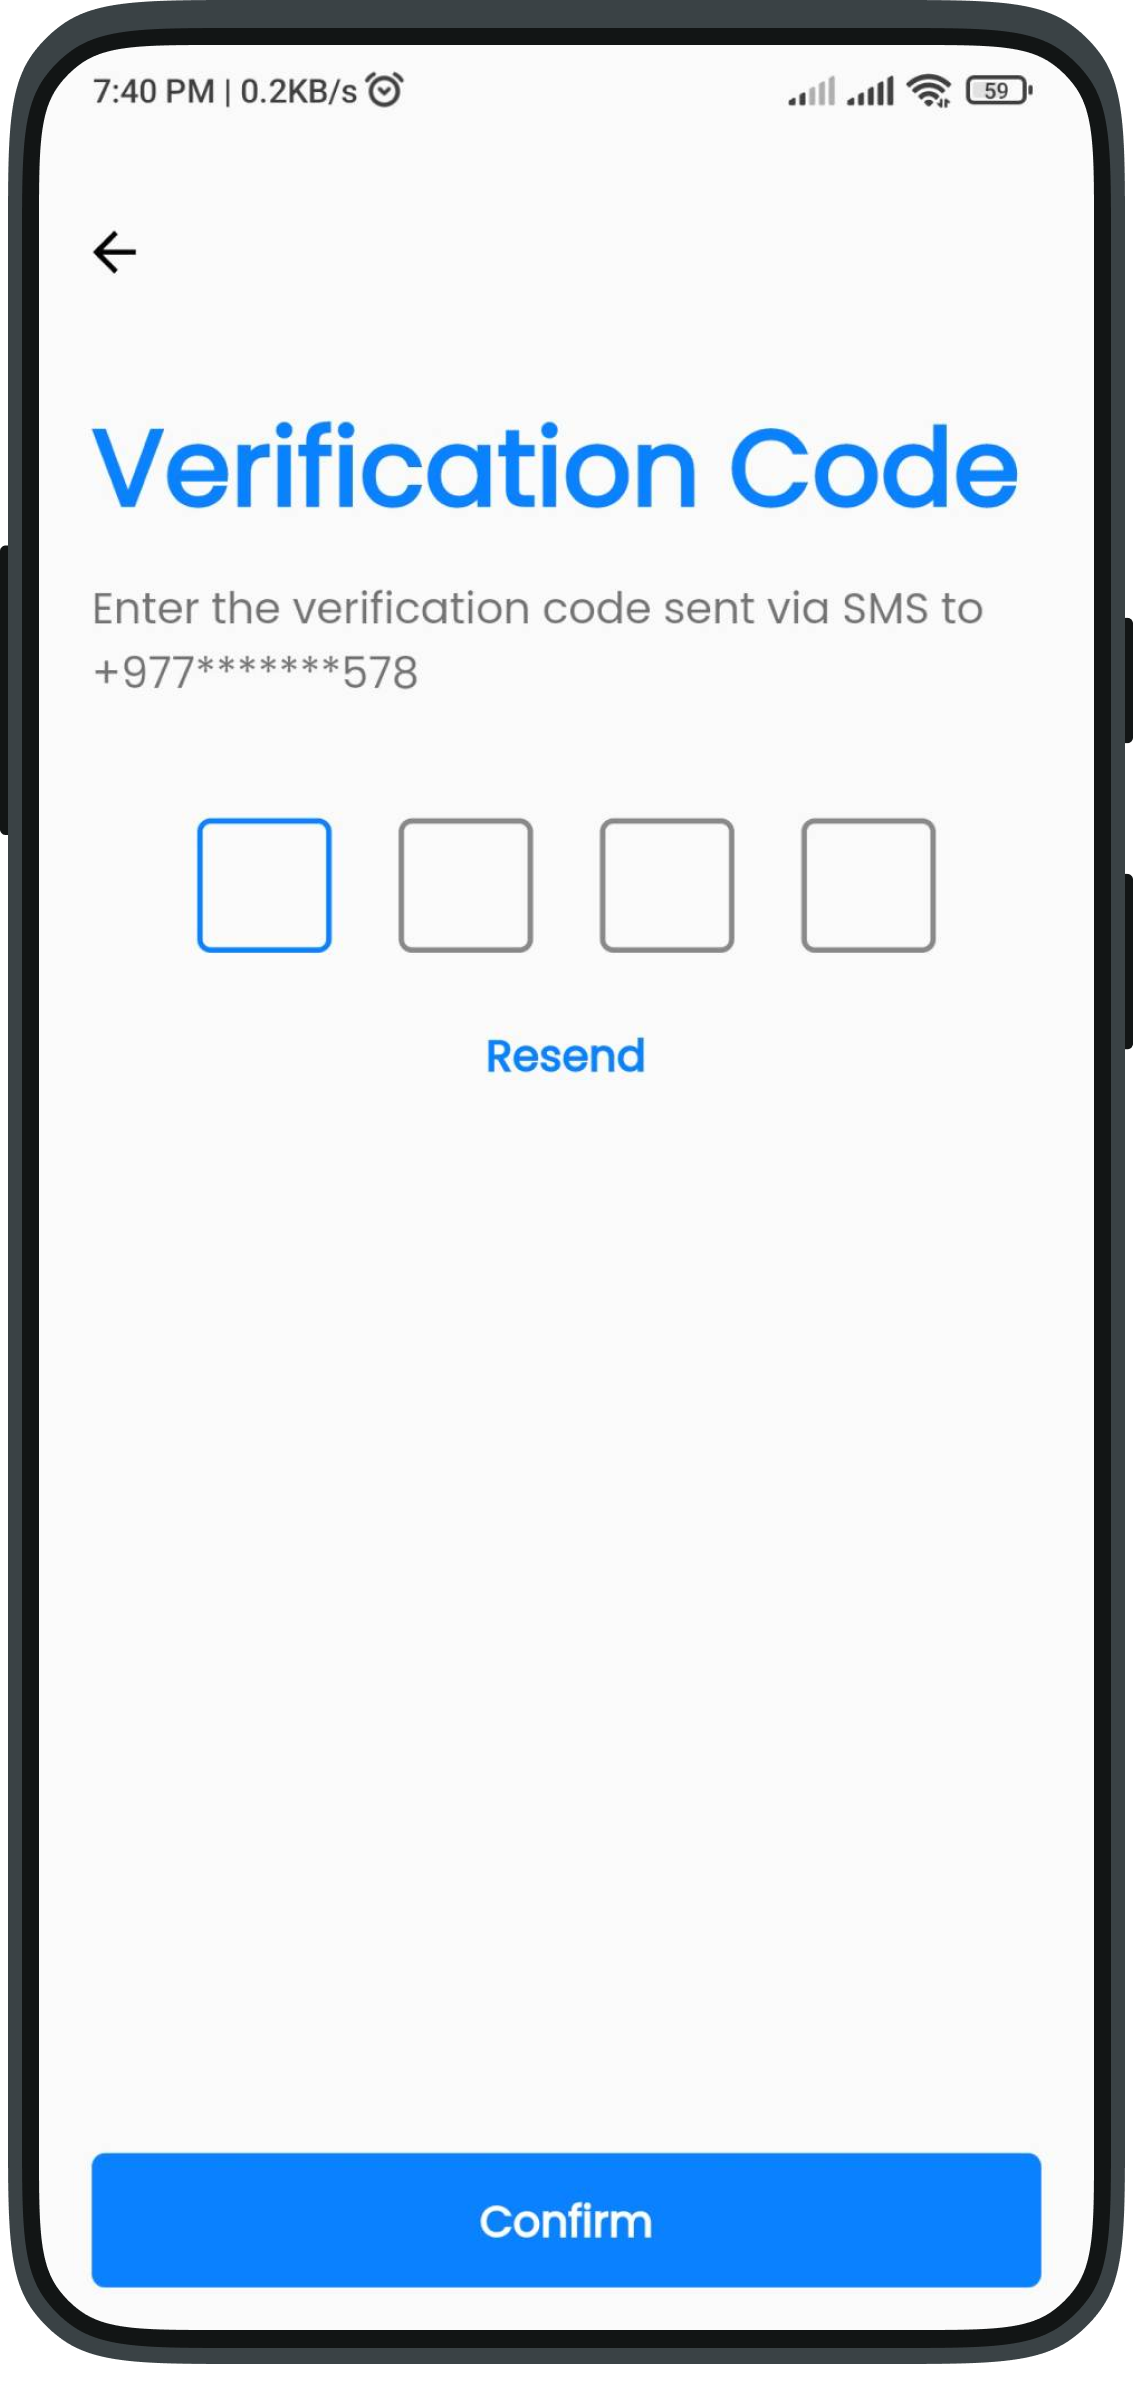
\includegraphics[width=0.6\linewidth]{images/results/mobile/OTP.png}
        \caption[Enter OTP Screen ]{Enter OTP Screen}
        \label{fig:OTP.png}
        \end{figure}
           \begin{figure}[H]
        \centering
        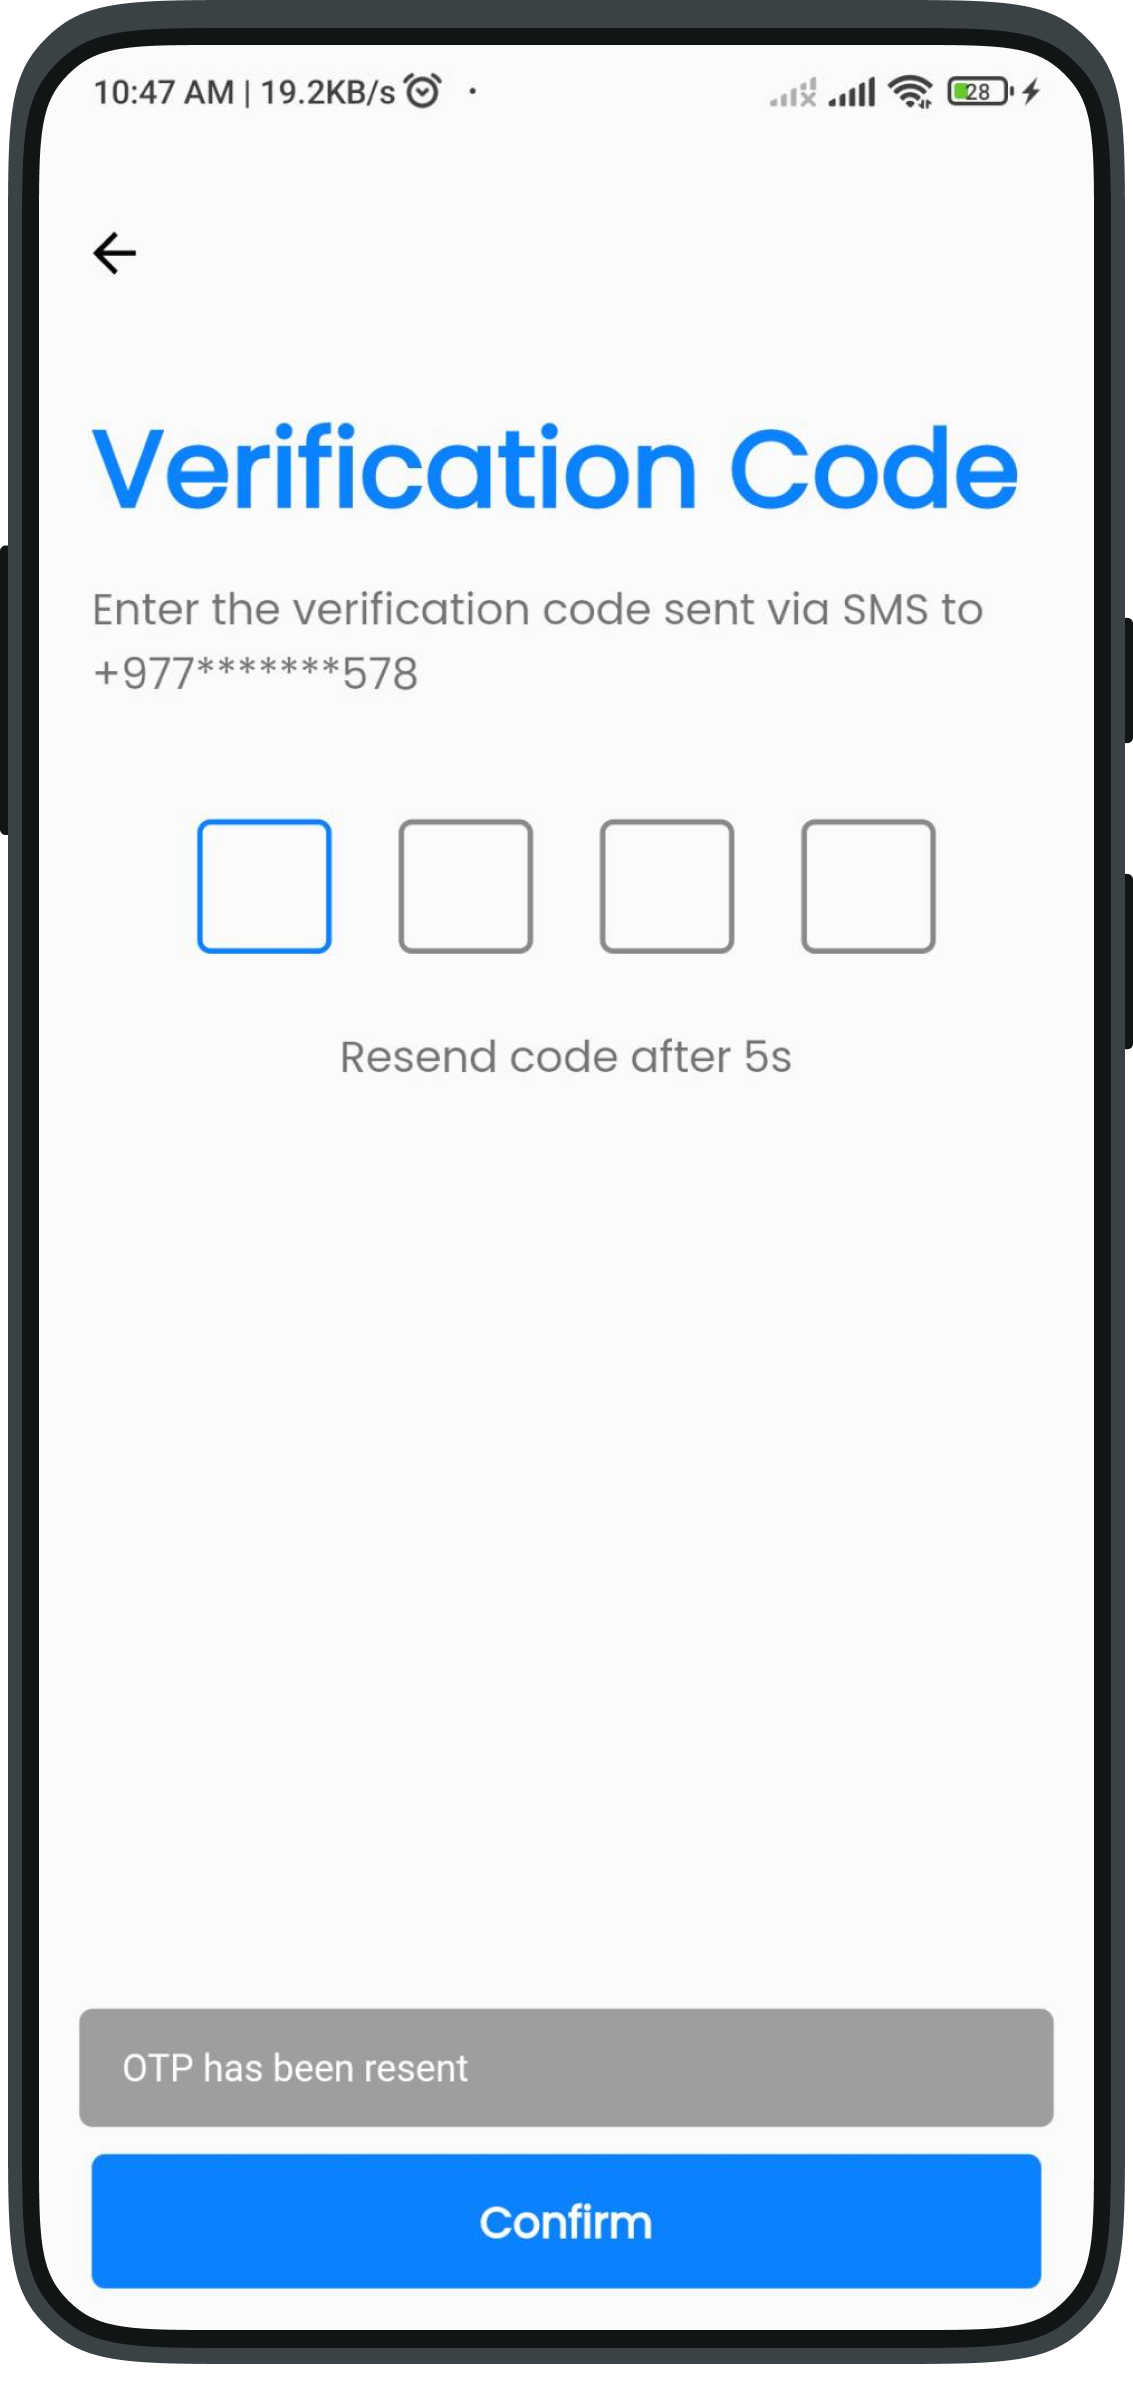
\includegraphics[width=0.6\linewidth]{images/results/mobile/OTPResend.png}
        \caption[Resend OTP Screen]{Resend OTP Screen}
        \label{fig:OTPResend.png}
        \end{figure}
        \end{multicols}

\textbf{Setting up MPIN}\\
    After validating the OTP, user can set up a pin which can be used for all other subsequent logins by the user.
    \begin{figure}[H]
    \centering
    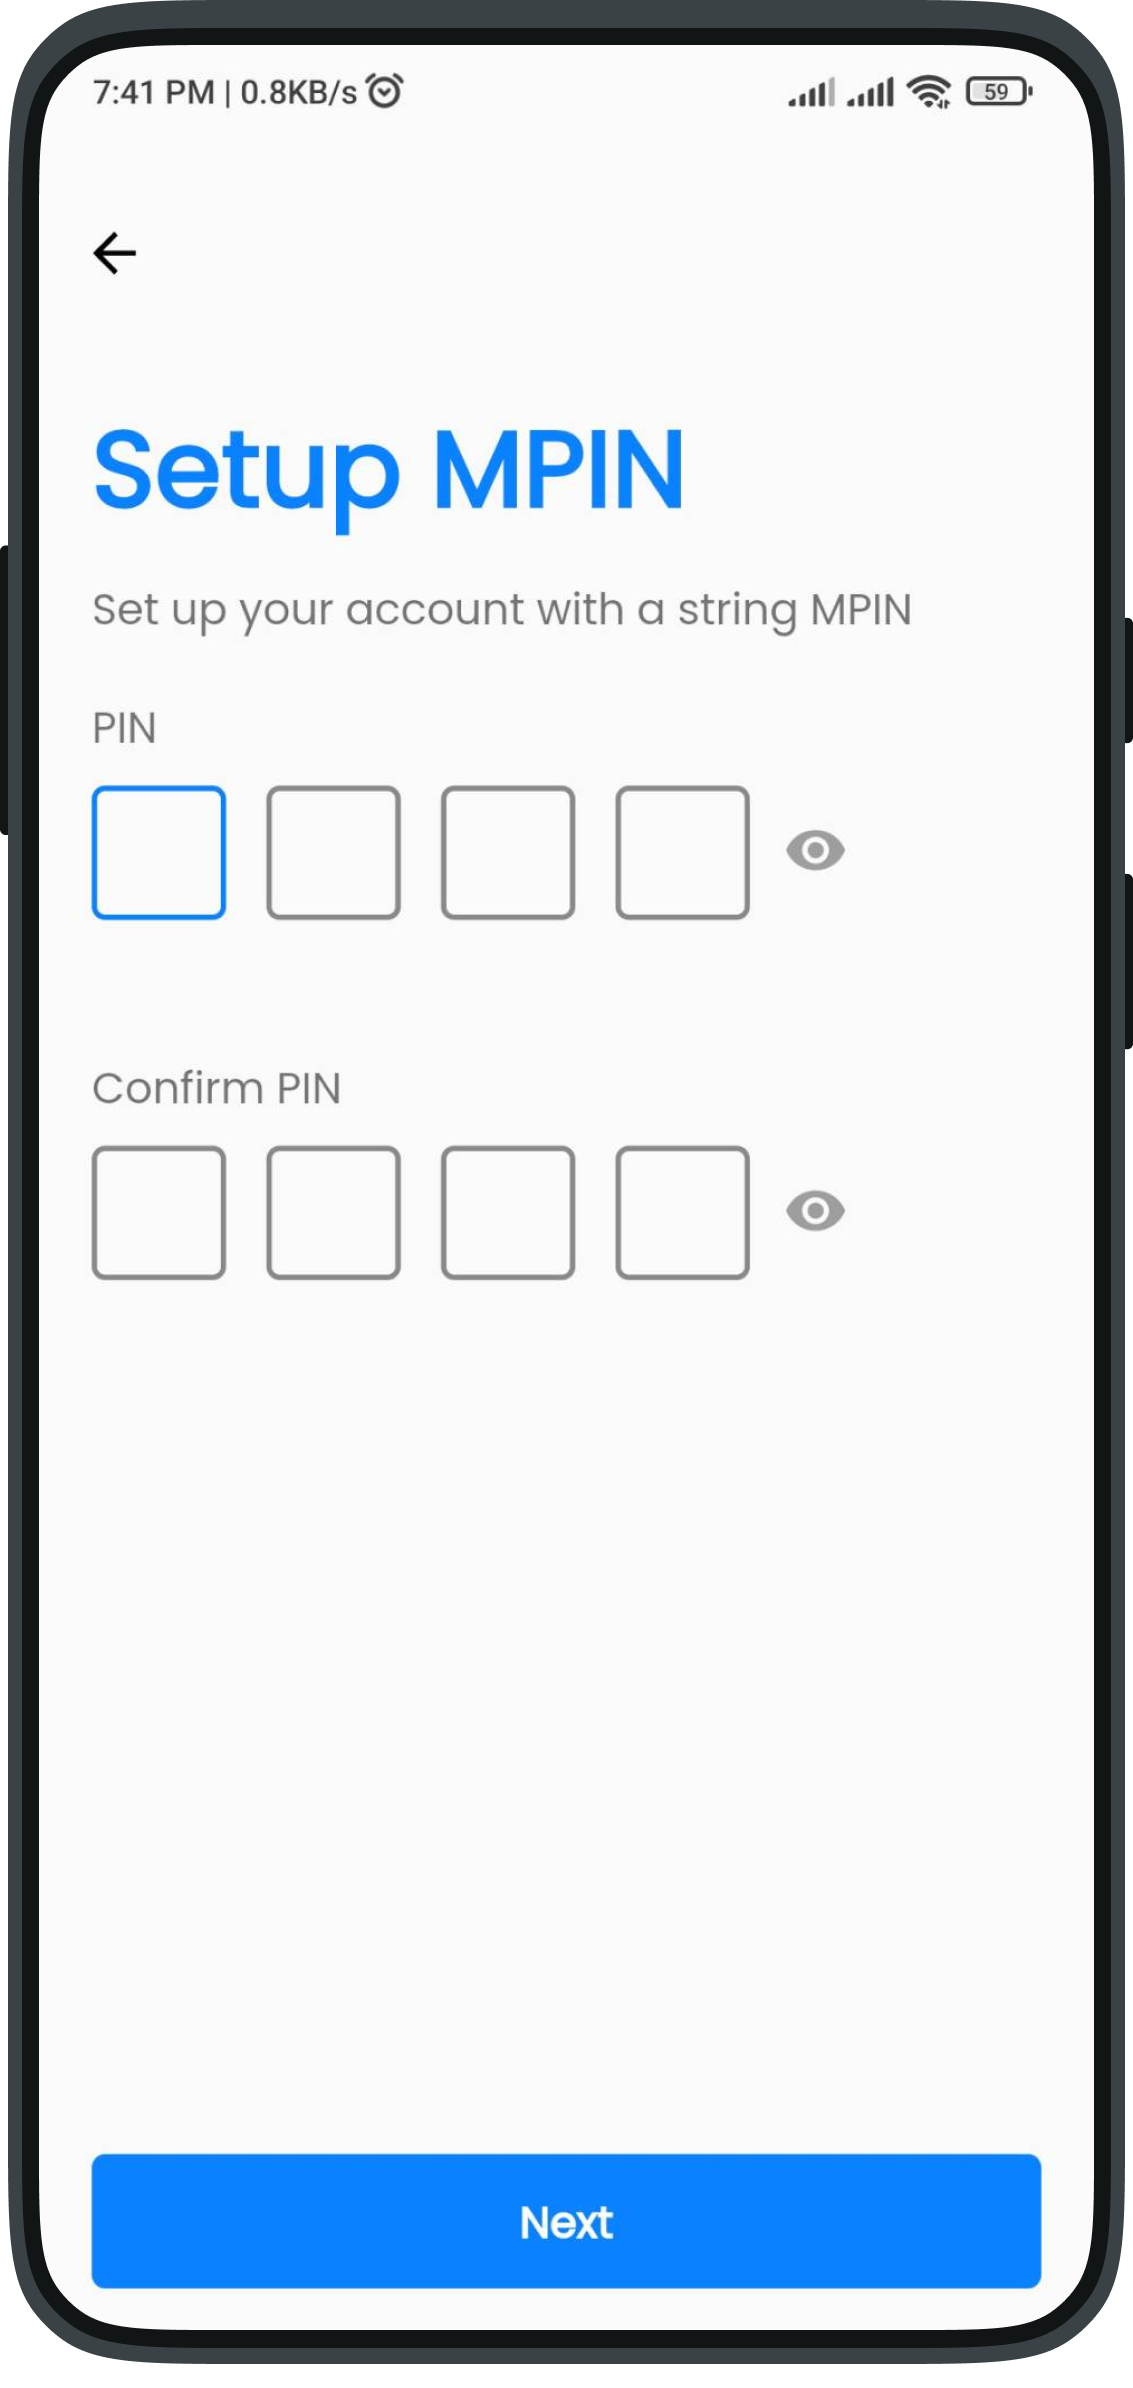
\includegraphics[width=0.3\linewidth]{images/results/mobile/SetupMPIN.png}
    \caption[Setup Pin]{Setup Pin}
    \label{fig:SetupMPIN.png}
    \end{figure}

\newpage
\textbf{Login with MPIN or Fingerprint}\\
    When user reopens the application, they are prompt to enter the mpin set during the initial login. They can also enable biometric login and use their fingerprint to login with instead of entering the mpin.
       \begin{figure}[H]
        \centering
        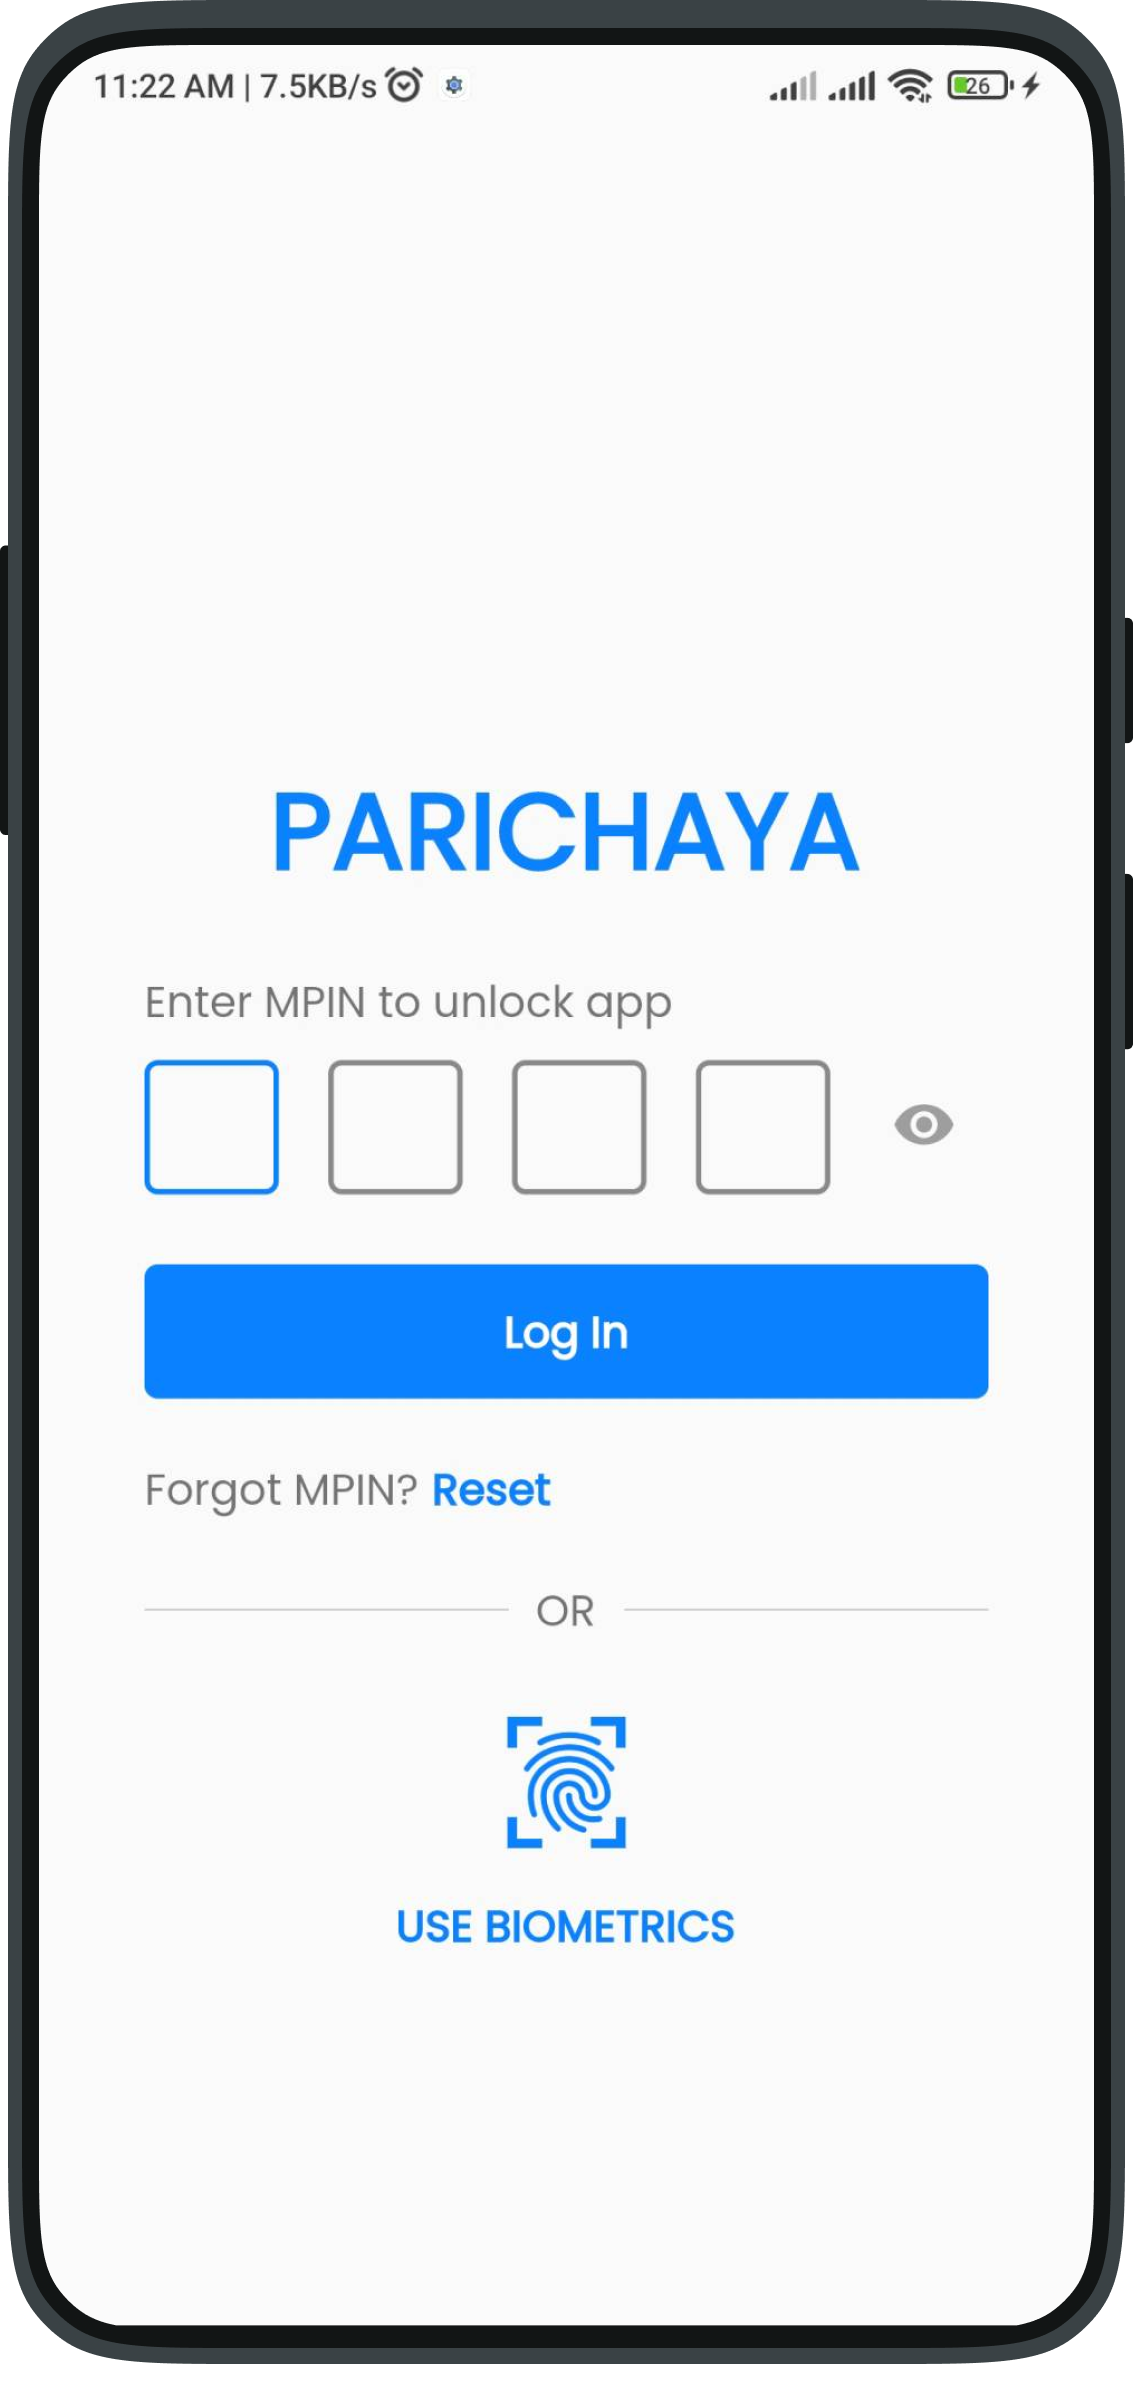
\includegraphics[width=0.3\linewidth]{images/results/mobile/LoginScreen.png}
        \caption[Login with MPIN Screen]{Login with MPIN Screen}
        \label{fig:LoginScreen.png}
        \end{figure}
    
\textbf{Forgot MPIN}\\
    In case the user forgets the mpin, they can opt to reset the mpin by entering the OTP sent to their mobile number. 
    \newpage
    \begin{multicols}{2} 
        \begin{figure}[H]
        \centering
        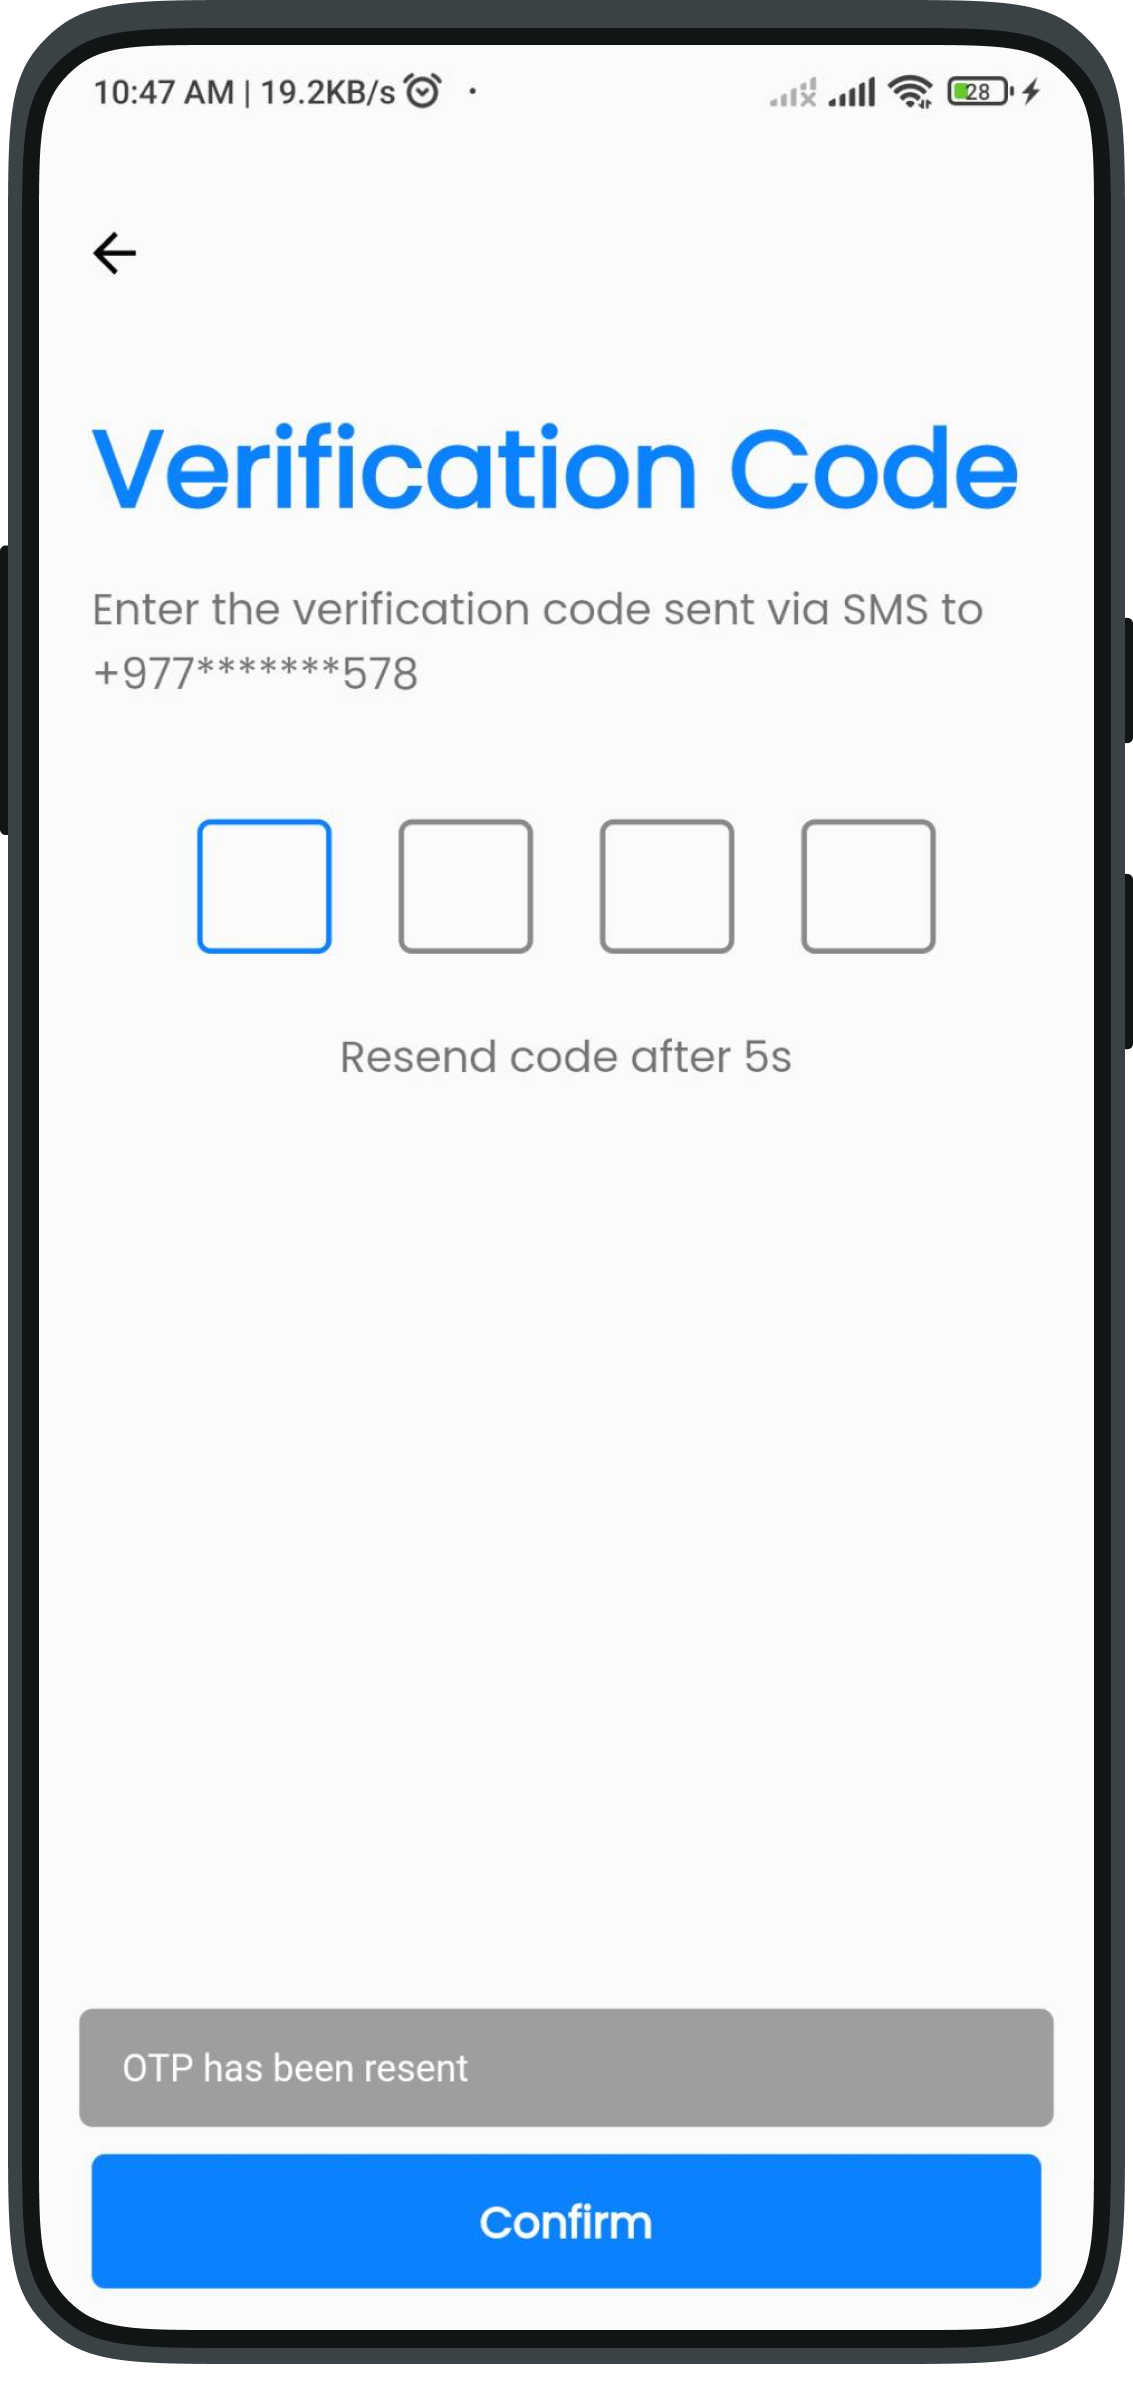
\includegraphics[width=0.6\linewidth]{images/results/mobile/OTPResend.png}
        \caption[Reset MPIN OTP Screen]{Reset MPIN OTP Screen}
        \label{fig:OTPResend.png}
        \end{figure}
        \begin{figure}[H]
        \centering
        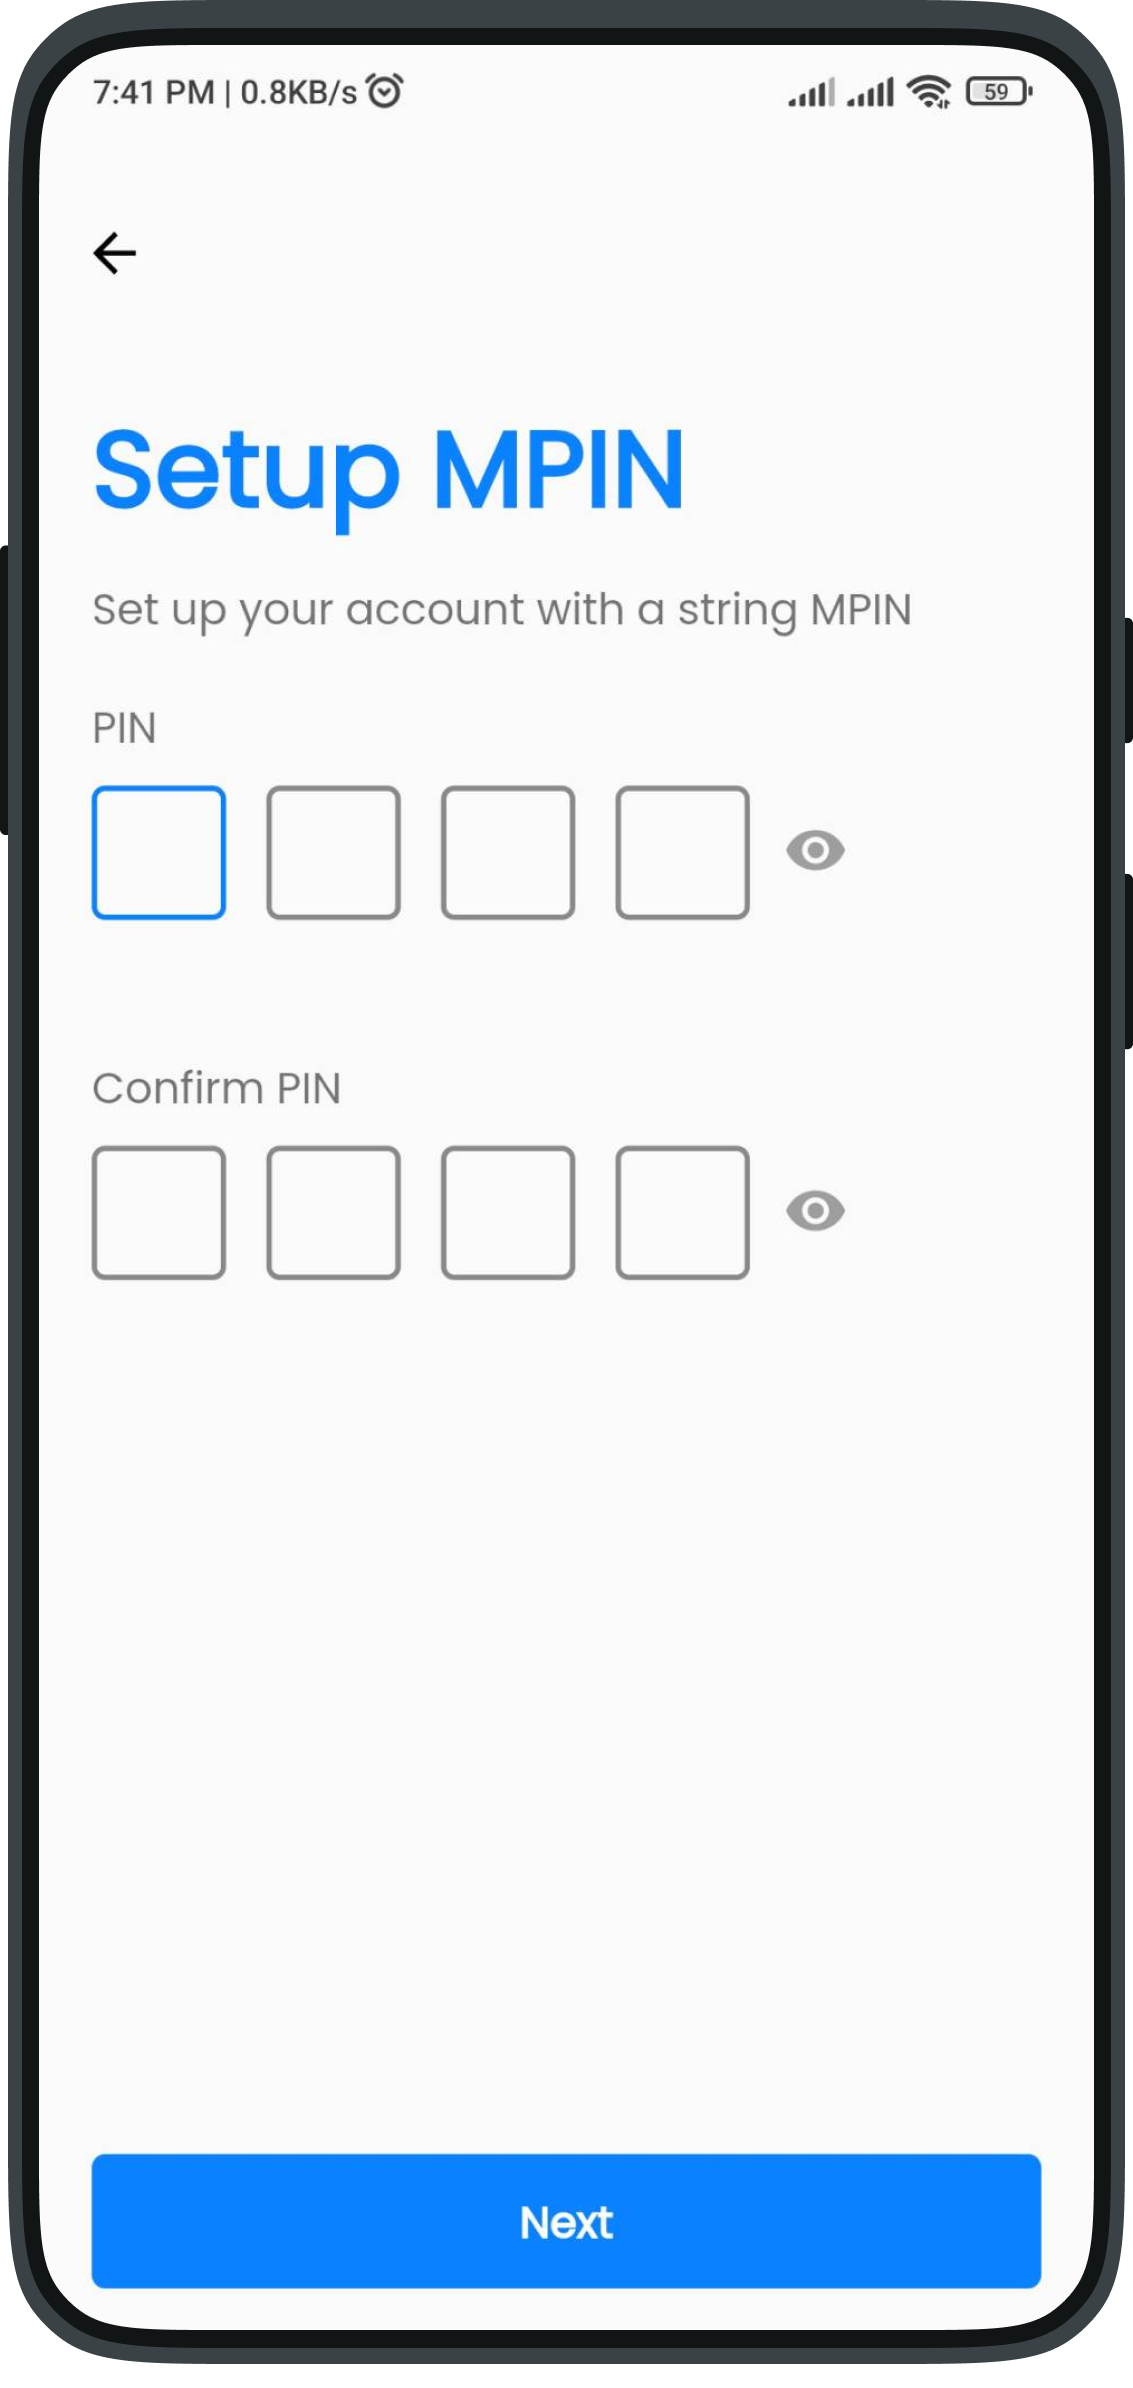
\includegraphics[width=0.6\linewidth]{images/results/mobile/SetupMPIN.png}
        \caption[Reset MPIN Screen]{Reset MPIN Screen}
        \label{fig:SetupMPIN.png}
        \end{figure}
      \end{multicols}
      
\textbf{Document View}\\
After completion of login process, user is navigated to the homescreen. Here, user can view the details of their documents and it's related card images.
\begin{multicols}{2}
    \begin{figure}[H]
        \centering
        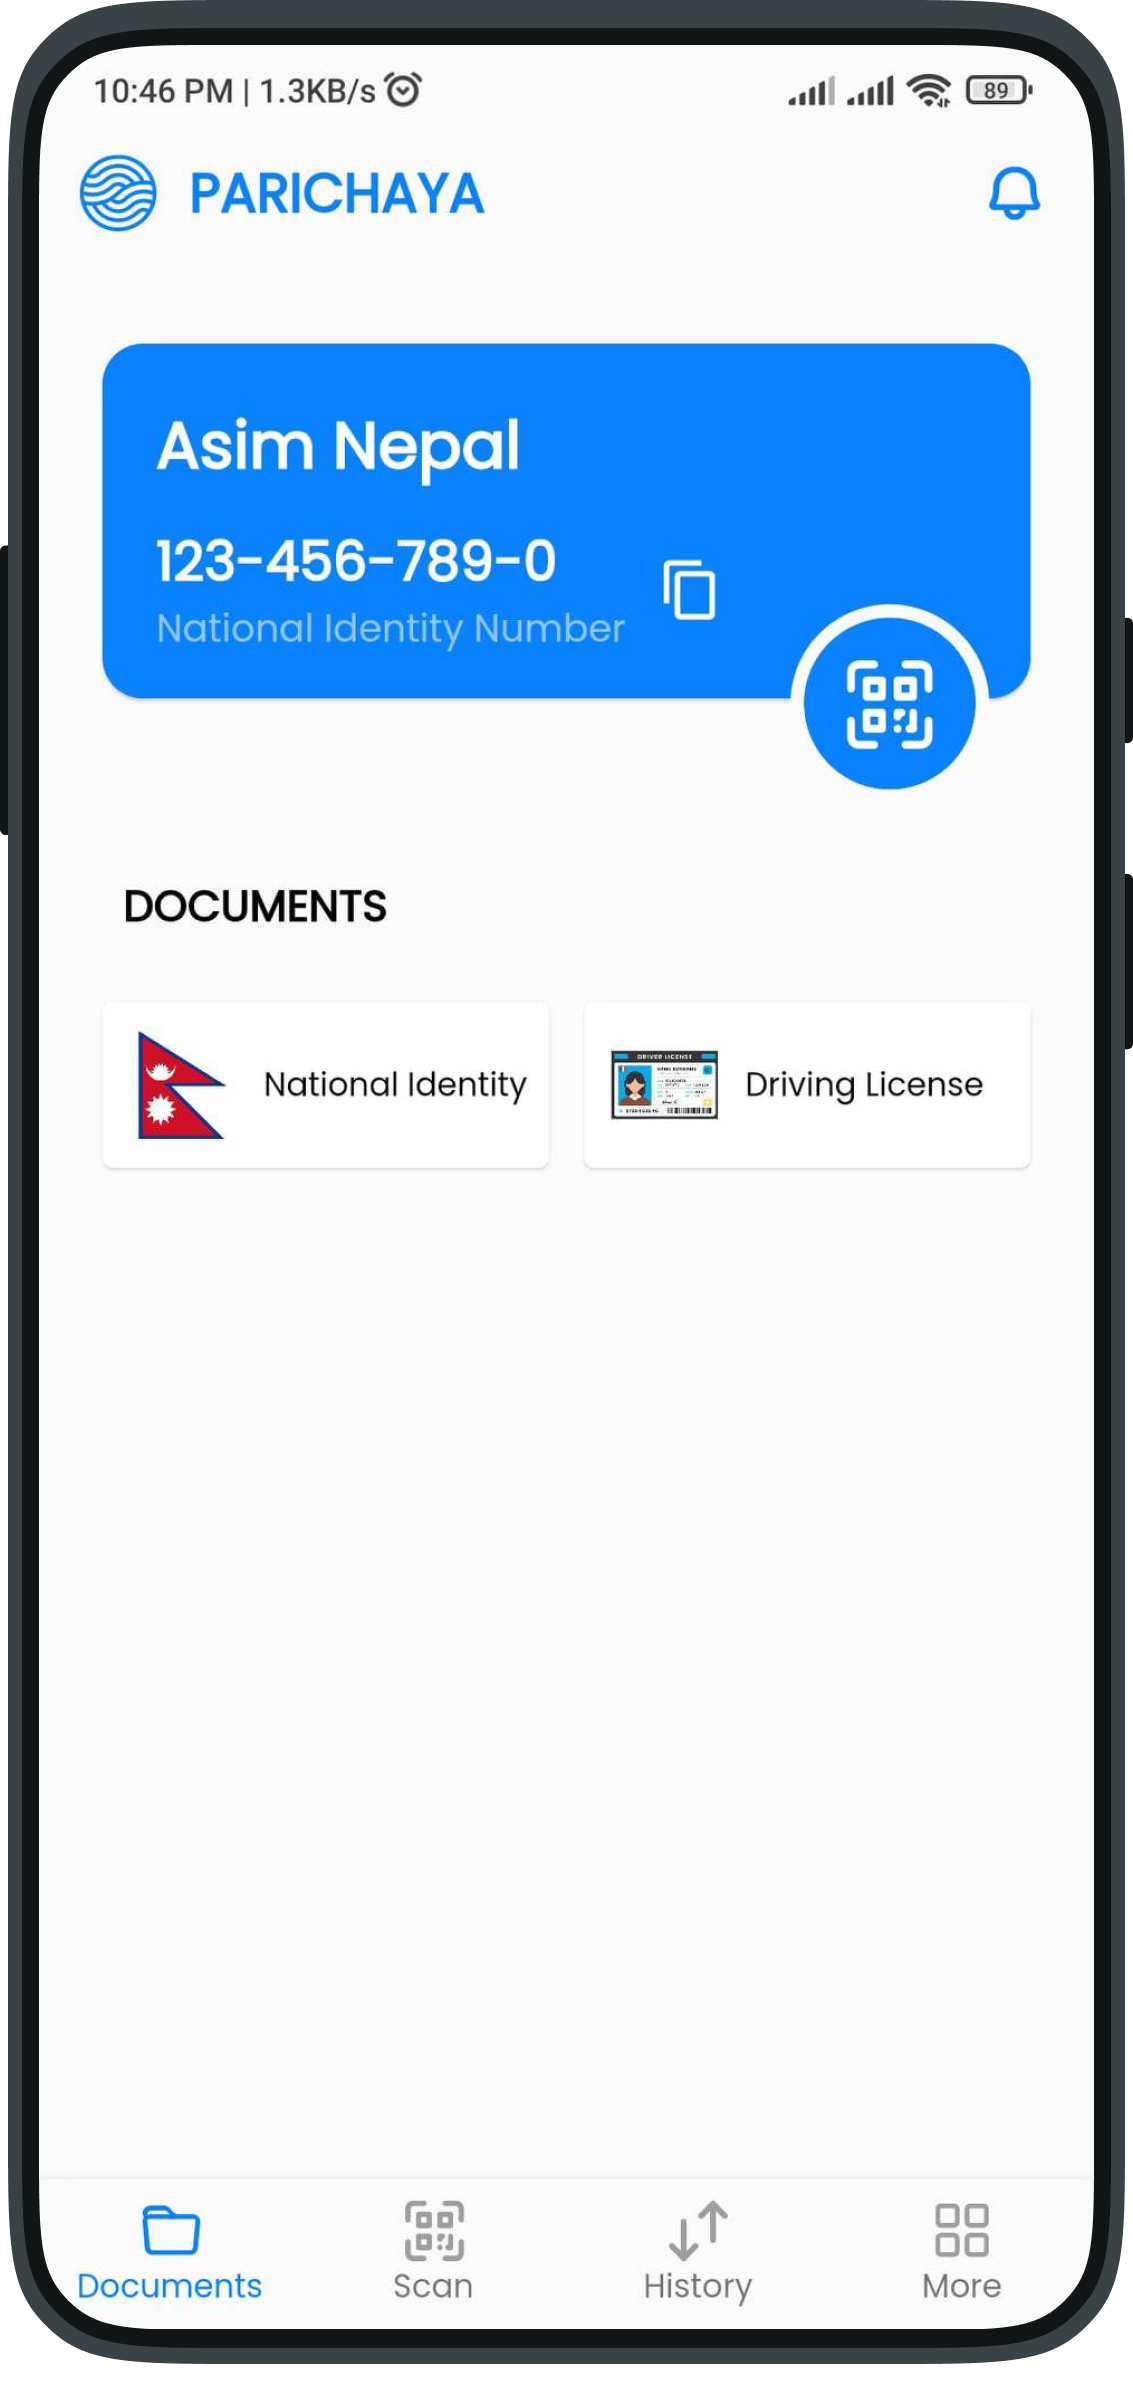
\includegraphics[width=0.6\linewidth]{images/results/mobile/Home.png}
        \caption[Document List View]{Document List View}
        \label{fig:Home.png}
        \end{figure} 
    \begin{figure}[H]
        \centering
        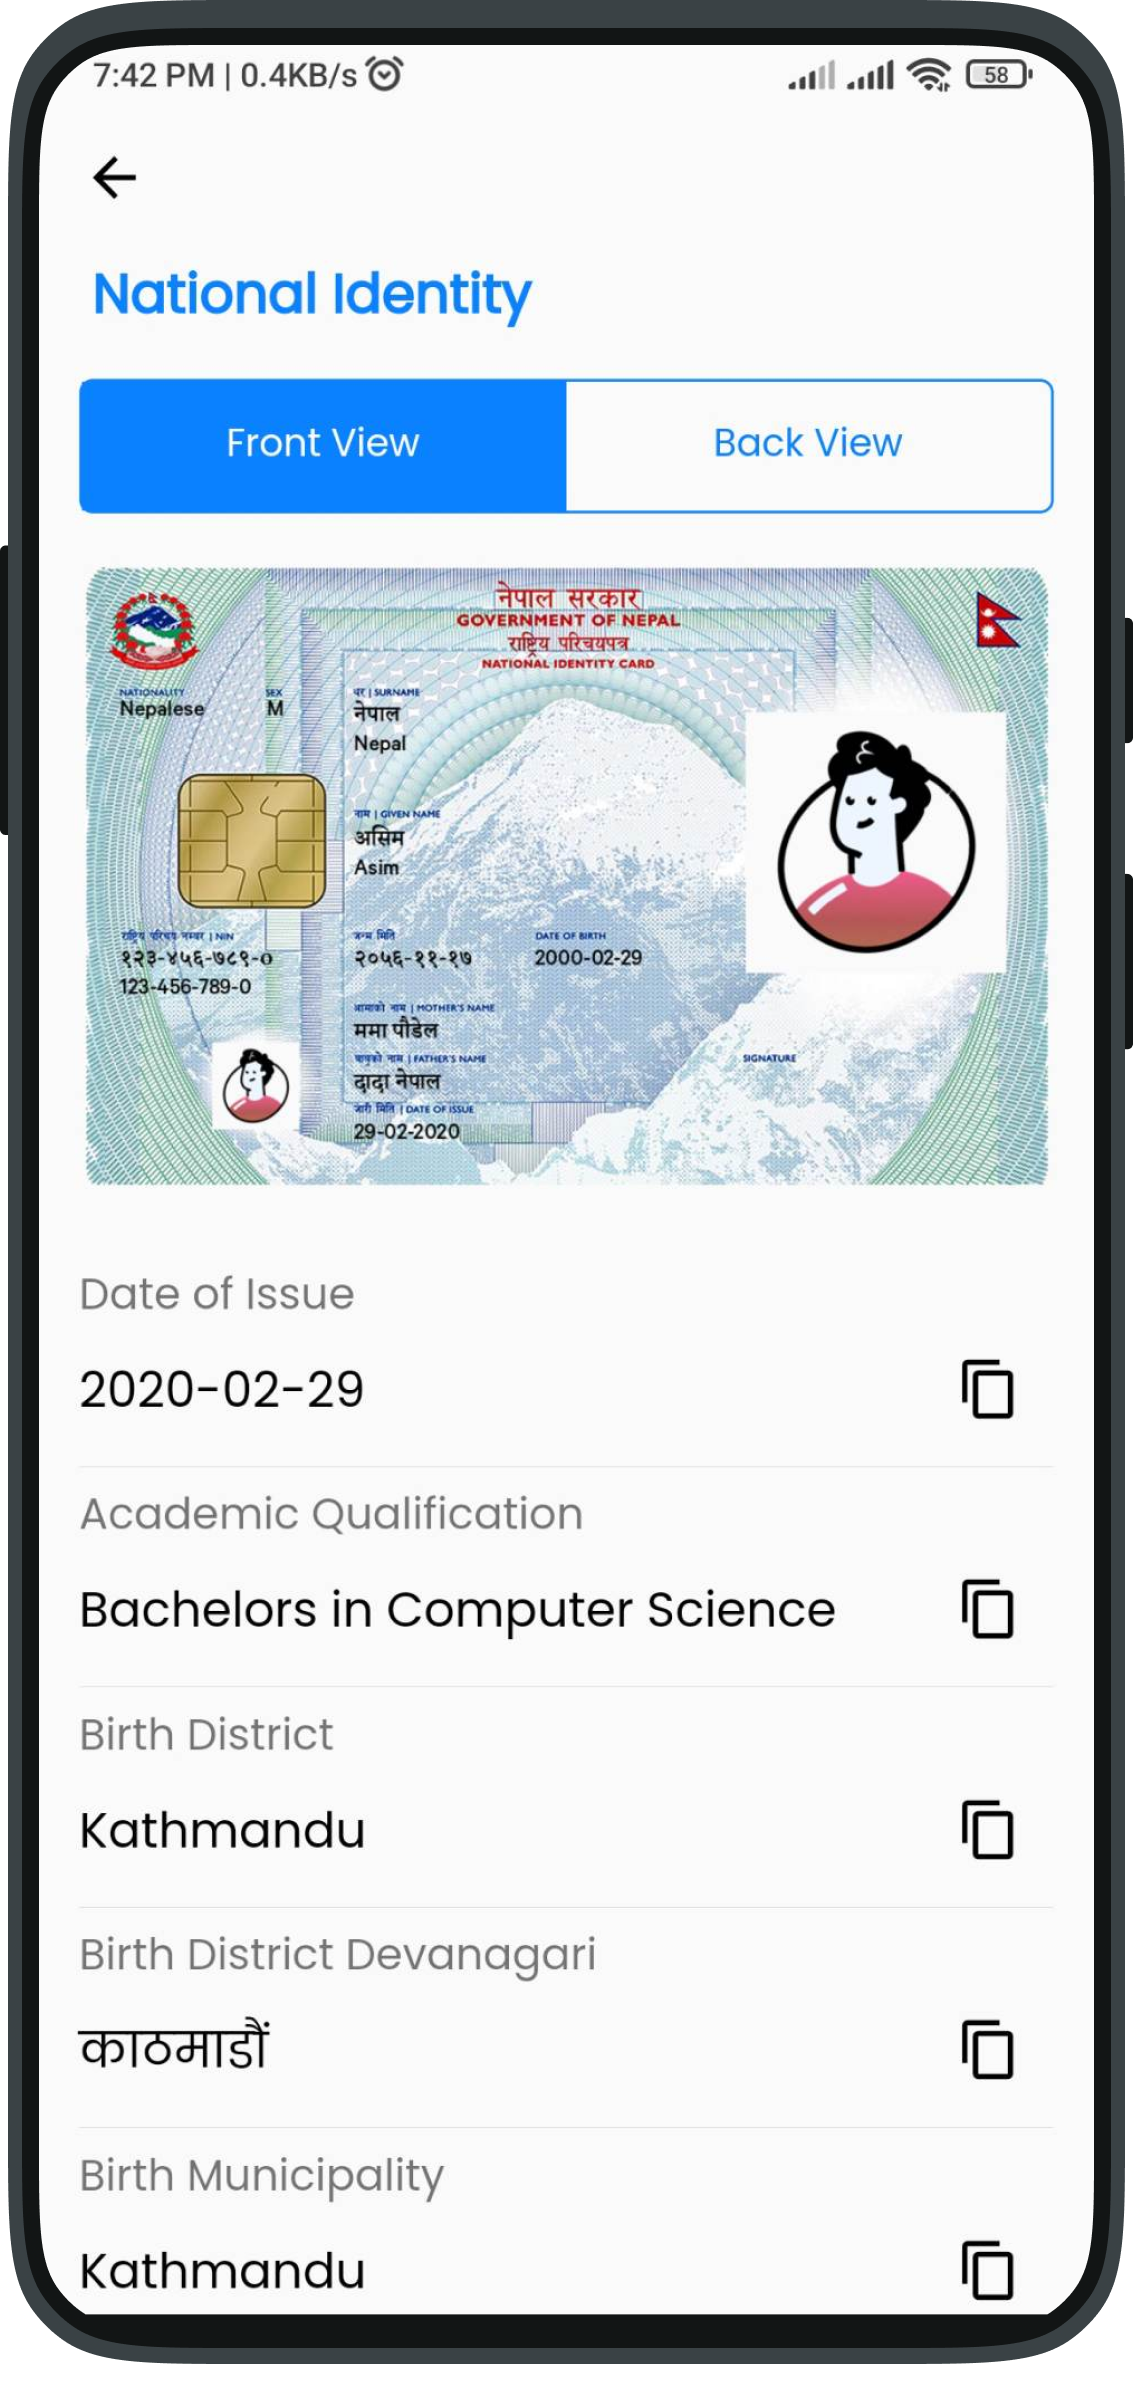
\includegraphics[width=0.6\linewidth]{images/results/mobile/NationalIdentity.png}
        \caption[Document Detail View ]{Document Detail View}
        \label{fig:NationalIdentity.png}
        \end{figure}     
\end{multicols}

\textbf{Document Share}\\
        User can share their driving license information to the traffic officer. Traffic police can either view it in user's phone or they can scan a QR code which contains driving license information.
        \begin{multicols}{2}
           \begin{figure}[H]
        \centering
        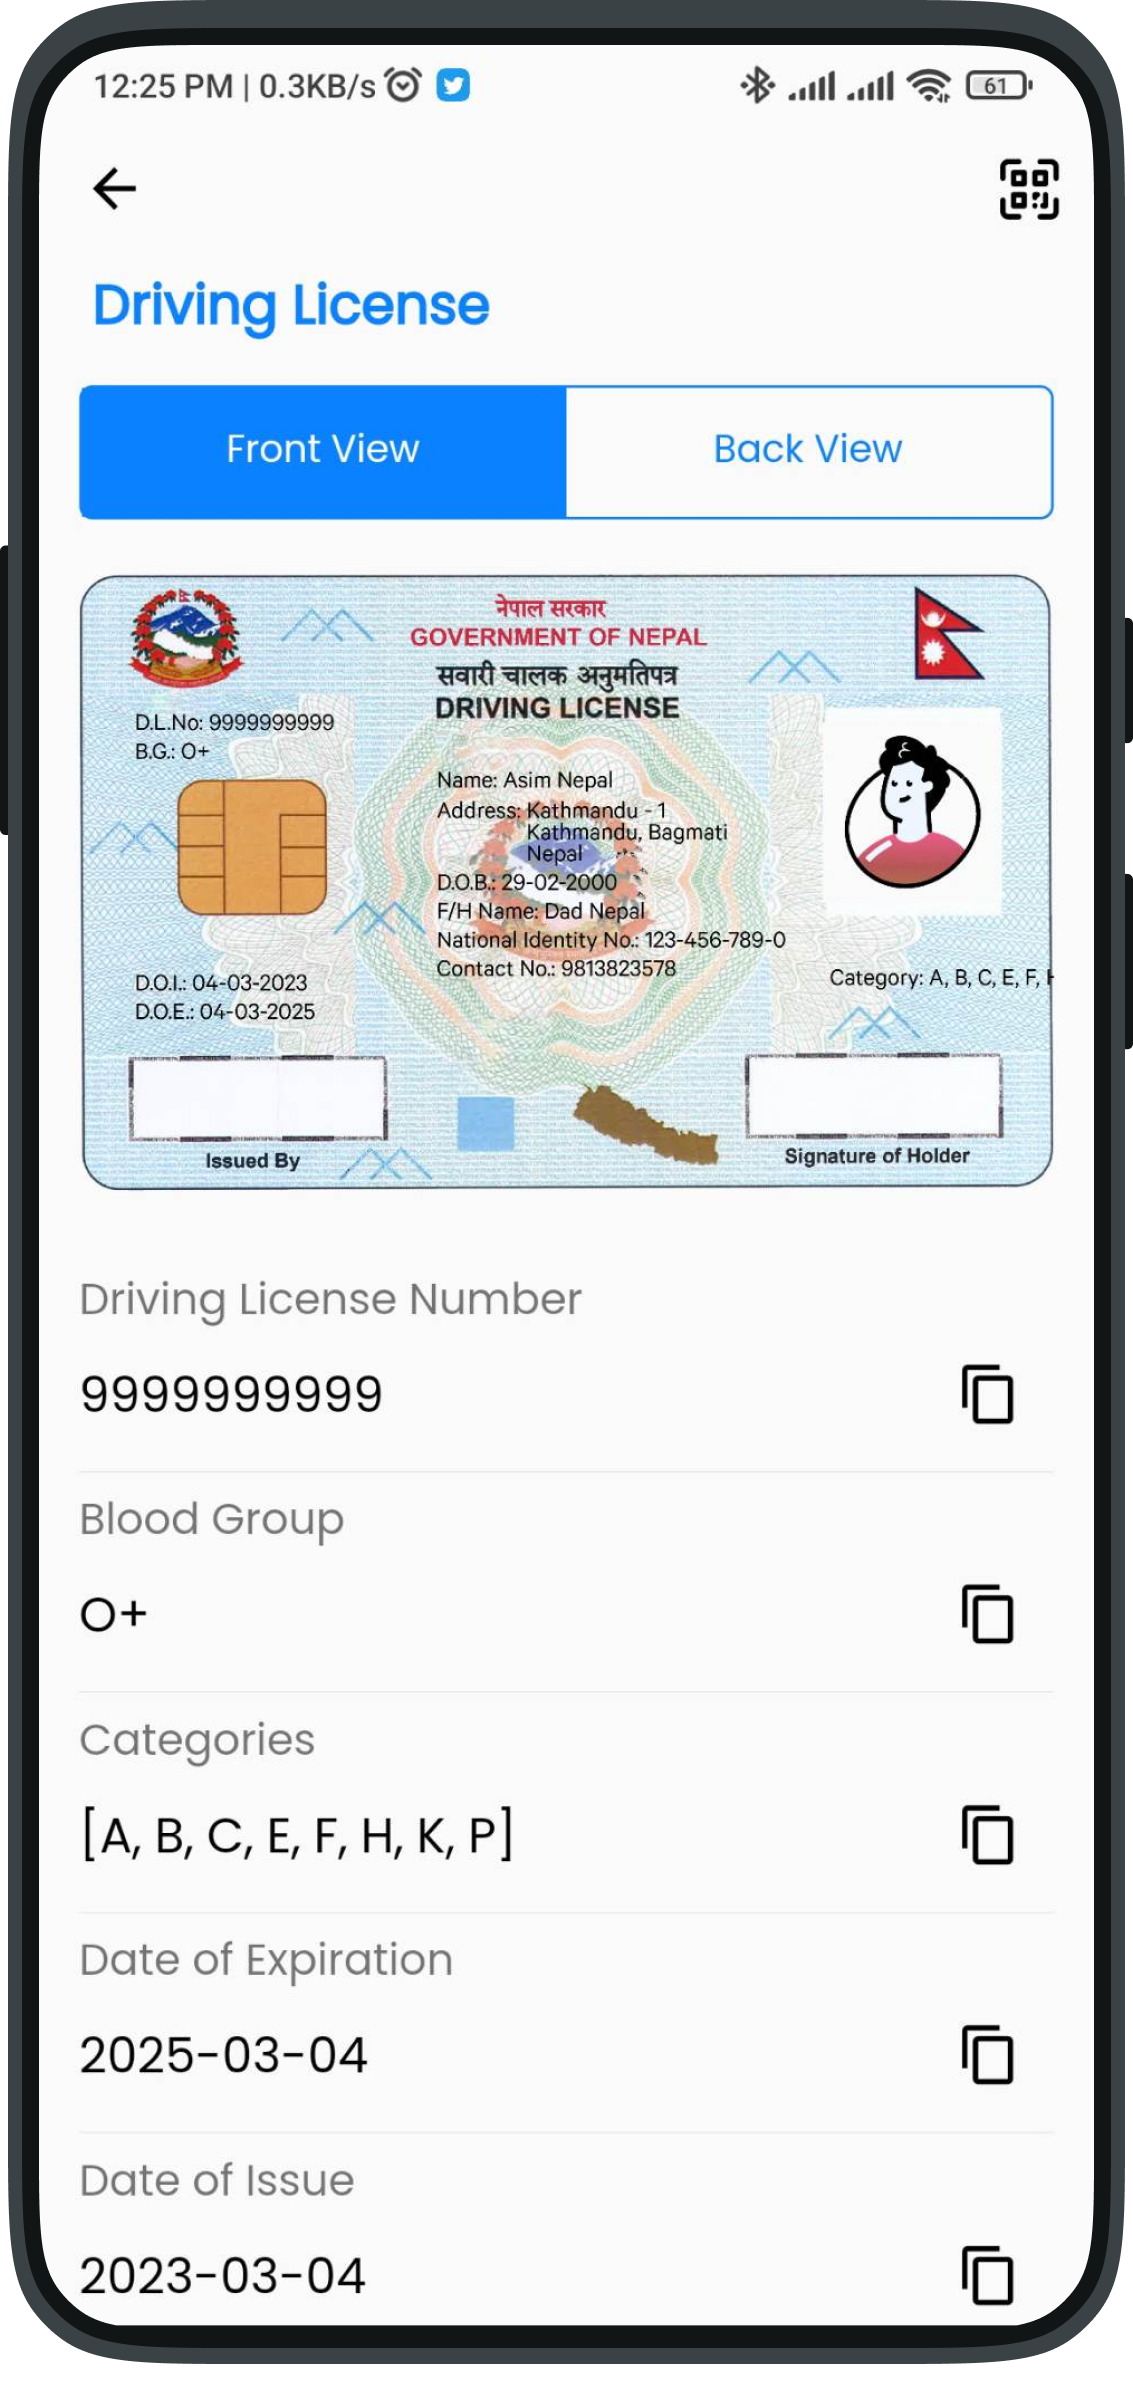
\includegraphics[width=0.6\linewidth]{images/results/mobile/DrivingLicense.png}
        \caption[Driving License ]{Driving License}
        \label{fig:DrivingLicense.png}
        \end{figure} 
        \begin{figure}[H]
        \centering
        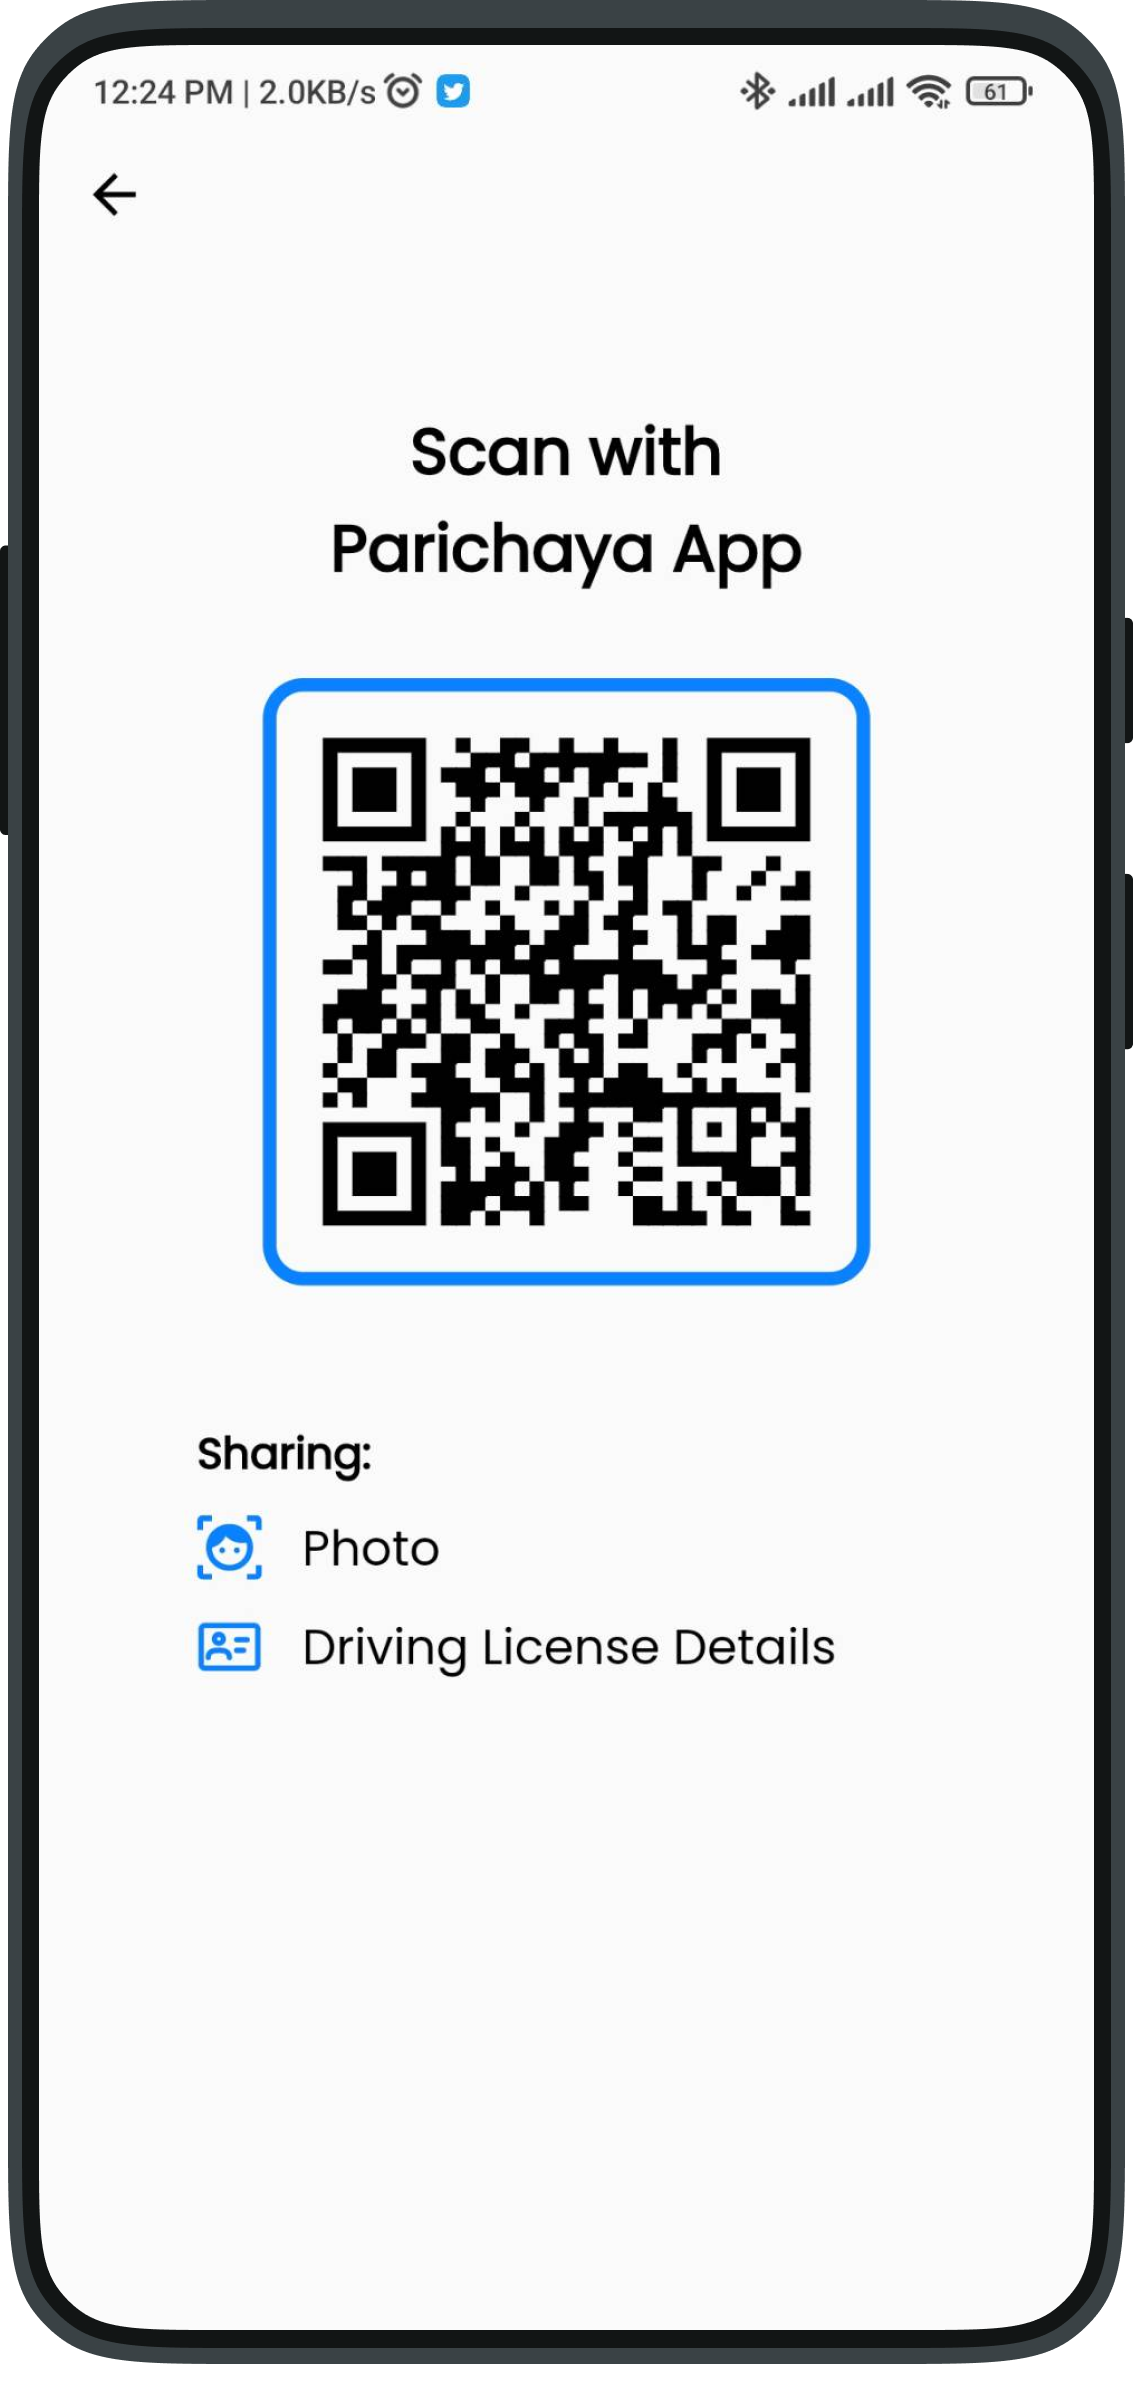
\includegraphics[width=0.6\linewidth]{images/results/mobile/DrivingLicenseQR.png}
        \caption[Share Driving License]{Share Driving License}
        \label{fig:DrivingLicenseQR.png}
        \end{figure} 
        \end{multicols}

        \textbf{Scan QR}\\
        The app contains a QR scanner which can be used to scan QR codes generated by the system to view the shared details of other users, or to share details to third party applications.
        \begin{figure}[H]
        \centering
        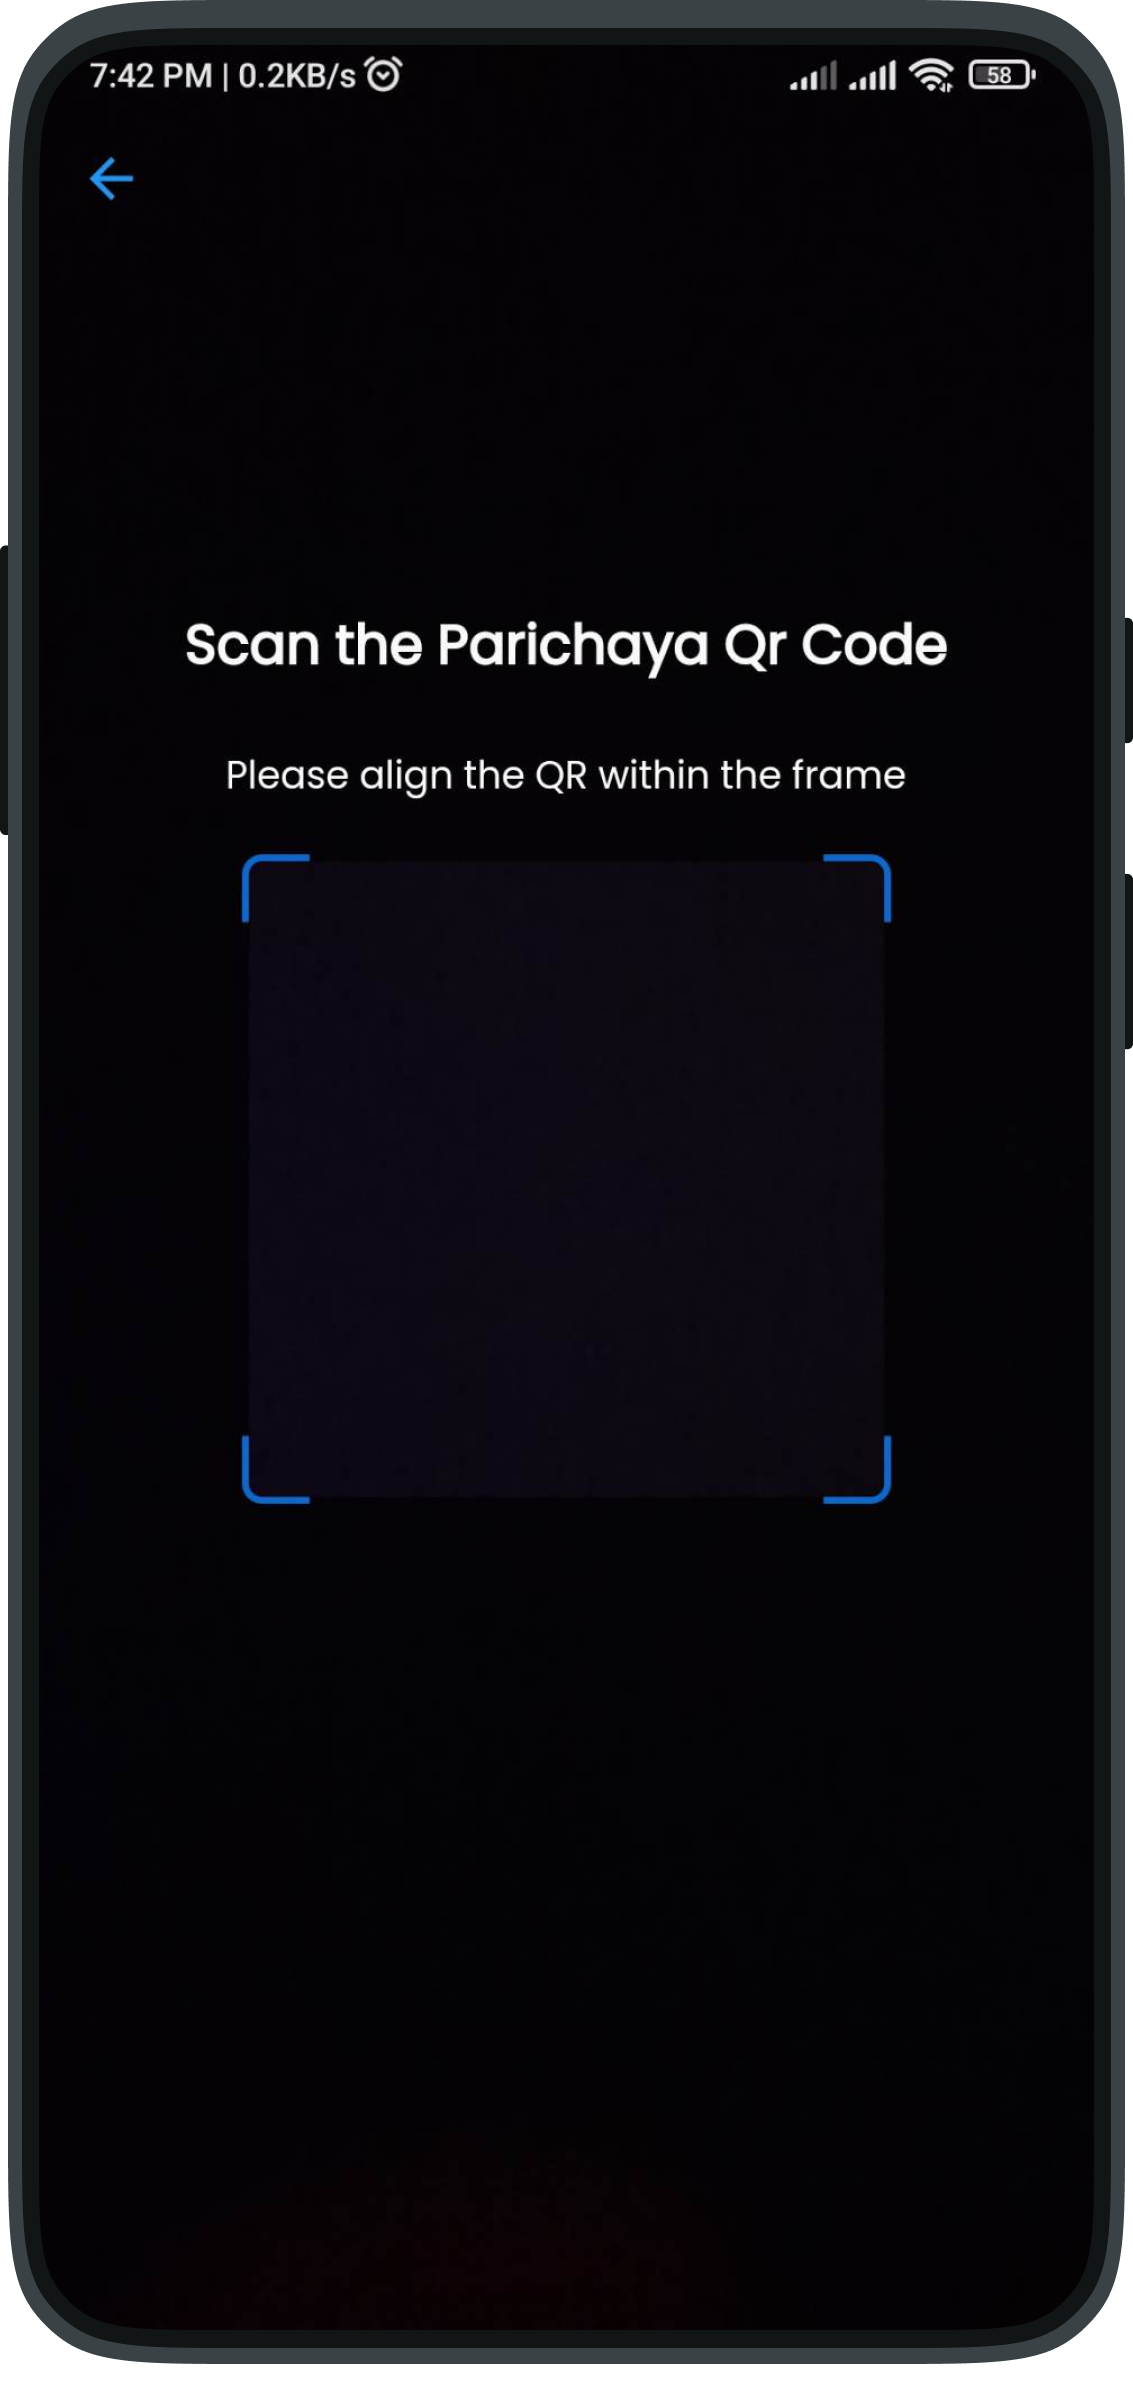
\includegraphics[width=0.3\linewidth]{images/results/mobile/QRScan.png}
        \caption[Scan QR Screen]{Scan QR Screen}
        \label{fig:QRScan.png}
        \end{figure}  
        
        \textbf{Age Verification}\\
        Verify Age is a basic feature for users to view their verified age. The user may share their age or driving license by generating the qr code with a touch of a button and the users who want to obtain this information can scan the qr code using Parichaya app. The user who shared the information will get real time update on who is viewing their data.
        \begin{multicols}{3}
            \begin{figure}[H]
            \centering
            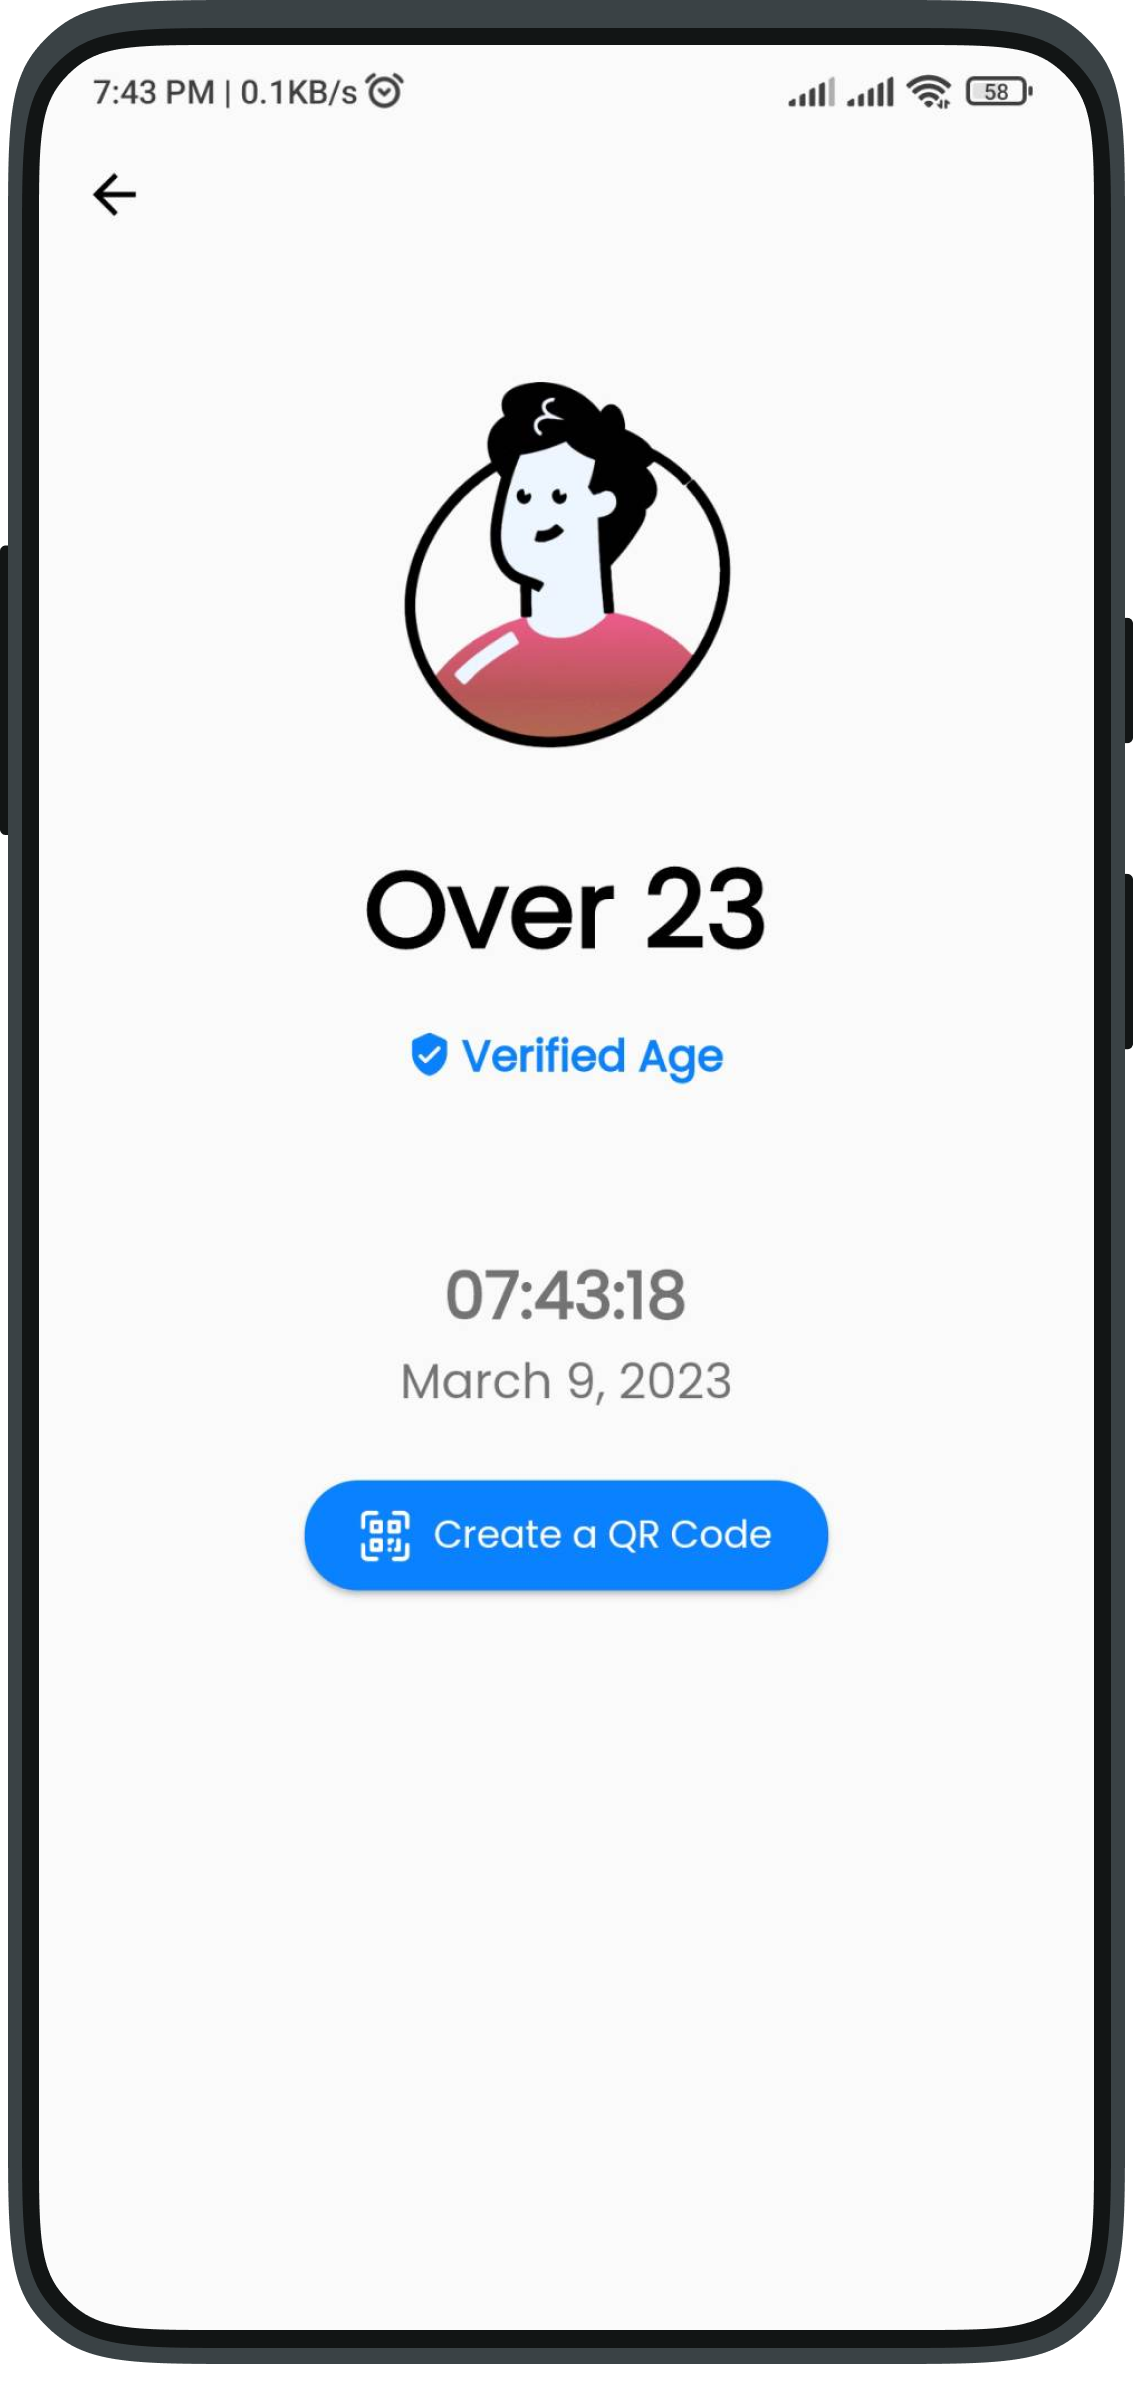
\includegraphics[width=0.8\linewidth]{images/results/mobile/VerifyAge.png}
            \caption[Verified Age]{Verified Age}
            \label{fig:VerifyAge.png}
            \end{figure}
              \begin{figure}[H]
            \centering
            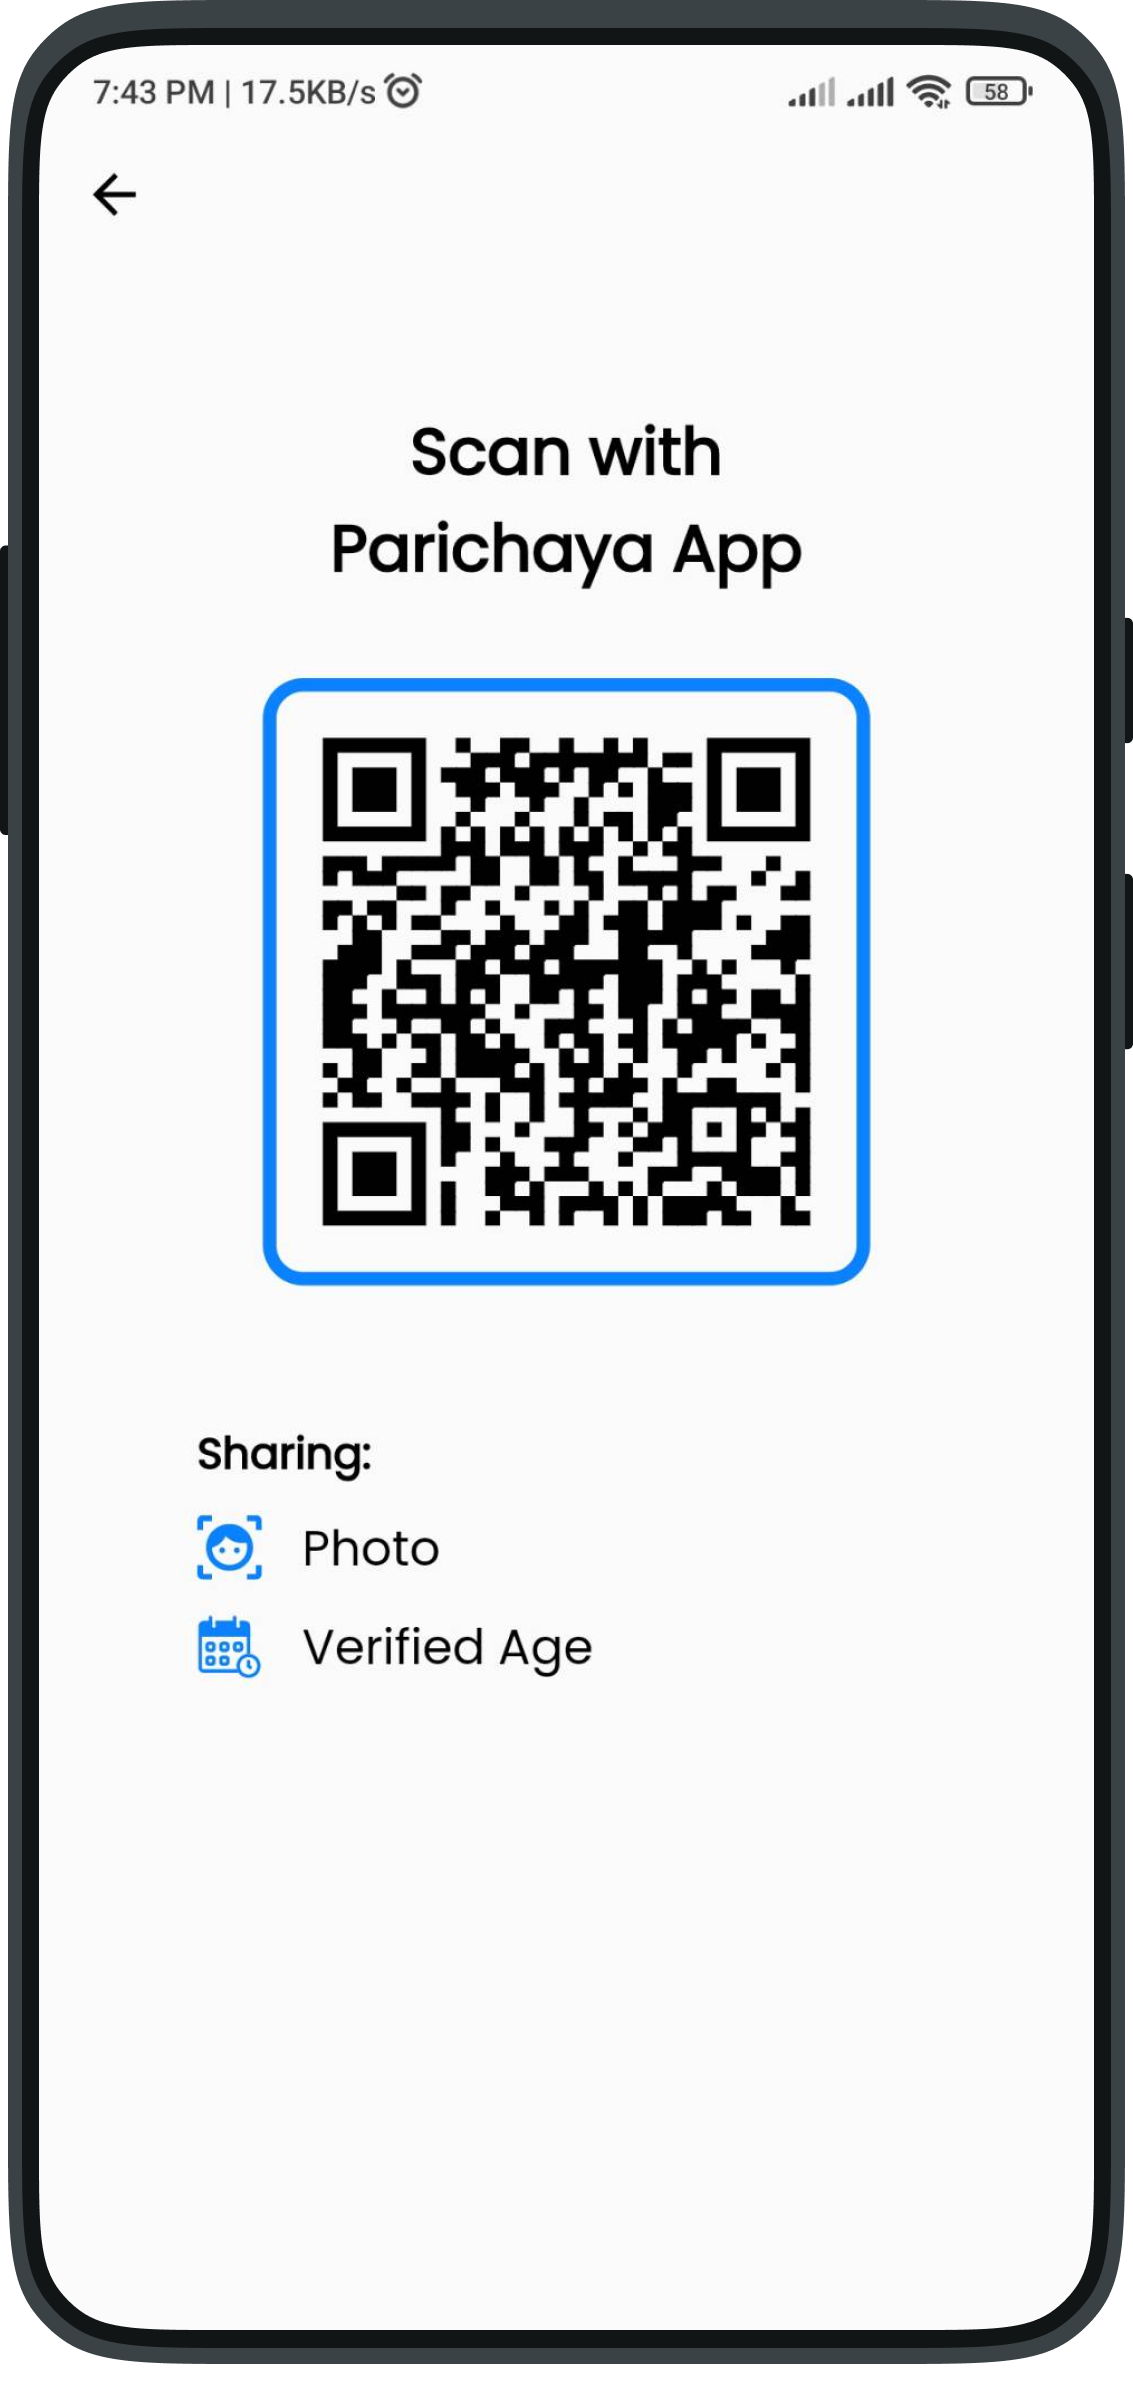
\includegraphics[width=0.8\linewidth]{images/results/mobile/VerifyAgeQR.png}
            \caption[Share Age]{Share Age}
            \label{fig:VerifyAgeQR.png}
            \end{figure}
              \begin{figure}[H]
            \centering
            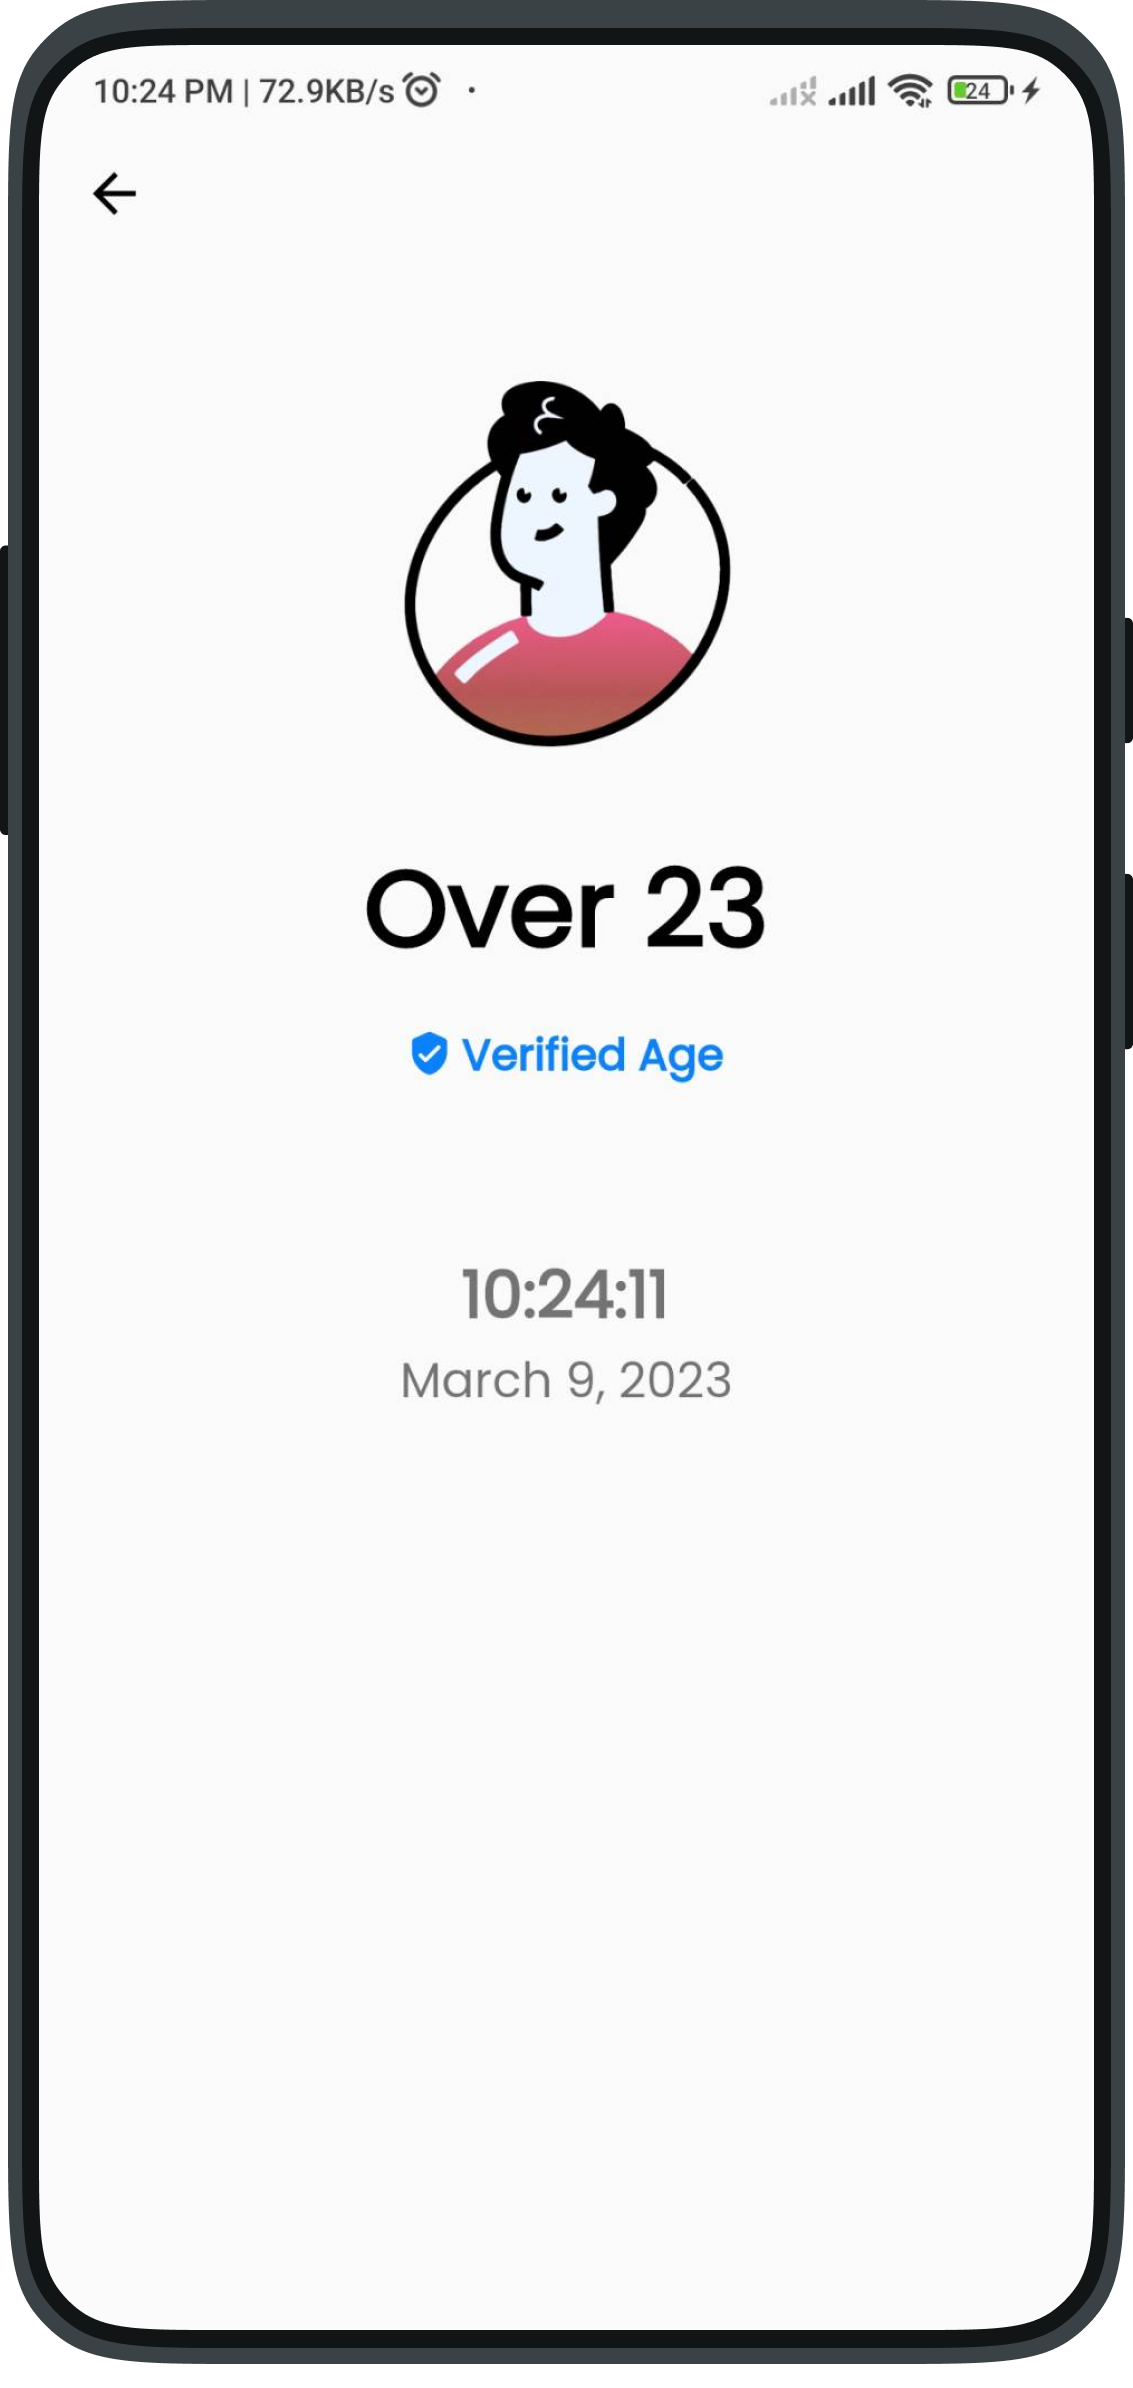
\includegraphics[width=0.8\linewidth]{images/results/mobile/VerifiedAgeShared.png}
            \caption[Shared Age]{Shared Age}
            \label{fig:VerifiedAgeShared.png}
            \end{figure}
            
        \end{multicols}
        \textbf{Document Share to Third Party Application}\\
        The user can share their information as required by third party applications. Here, the user scans the qr code generated by the third party (like banks) and will view all the information required to share. The user then may approve or deny the request.
         \begin{figure}[H]
            \centering
            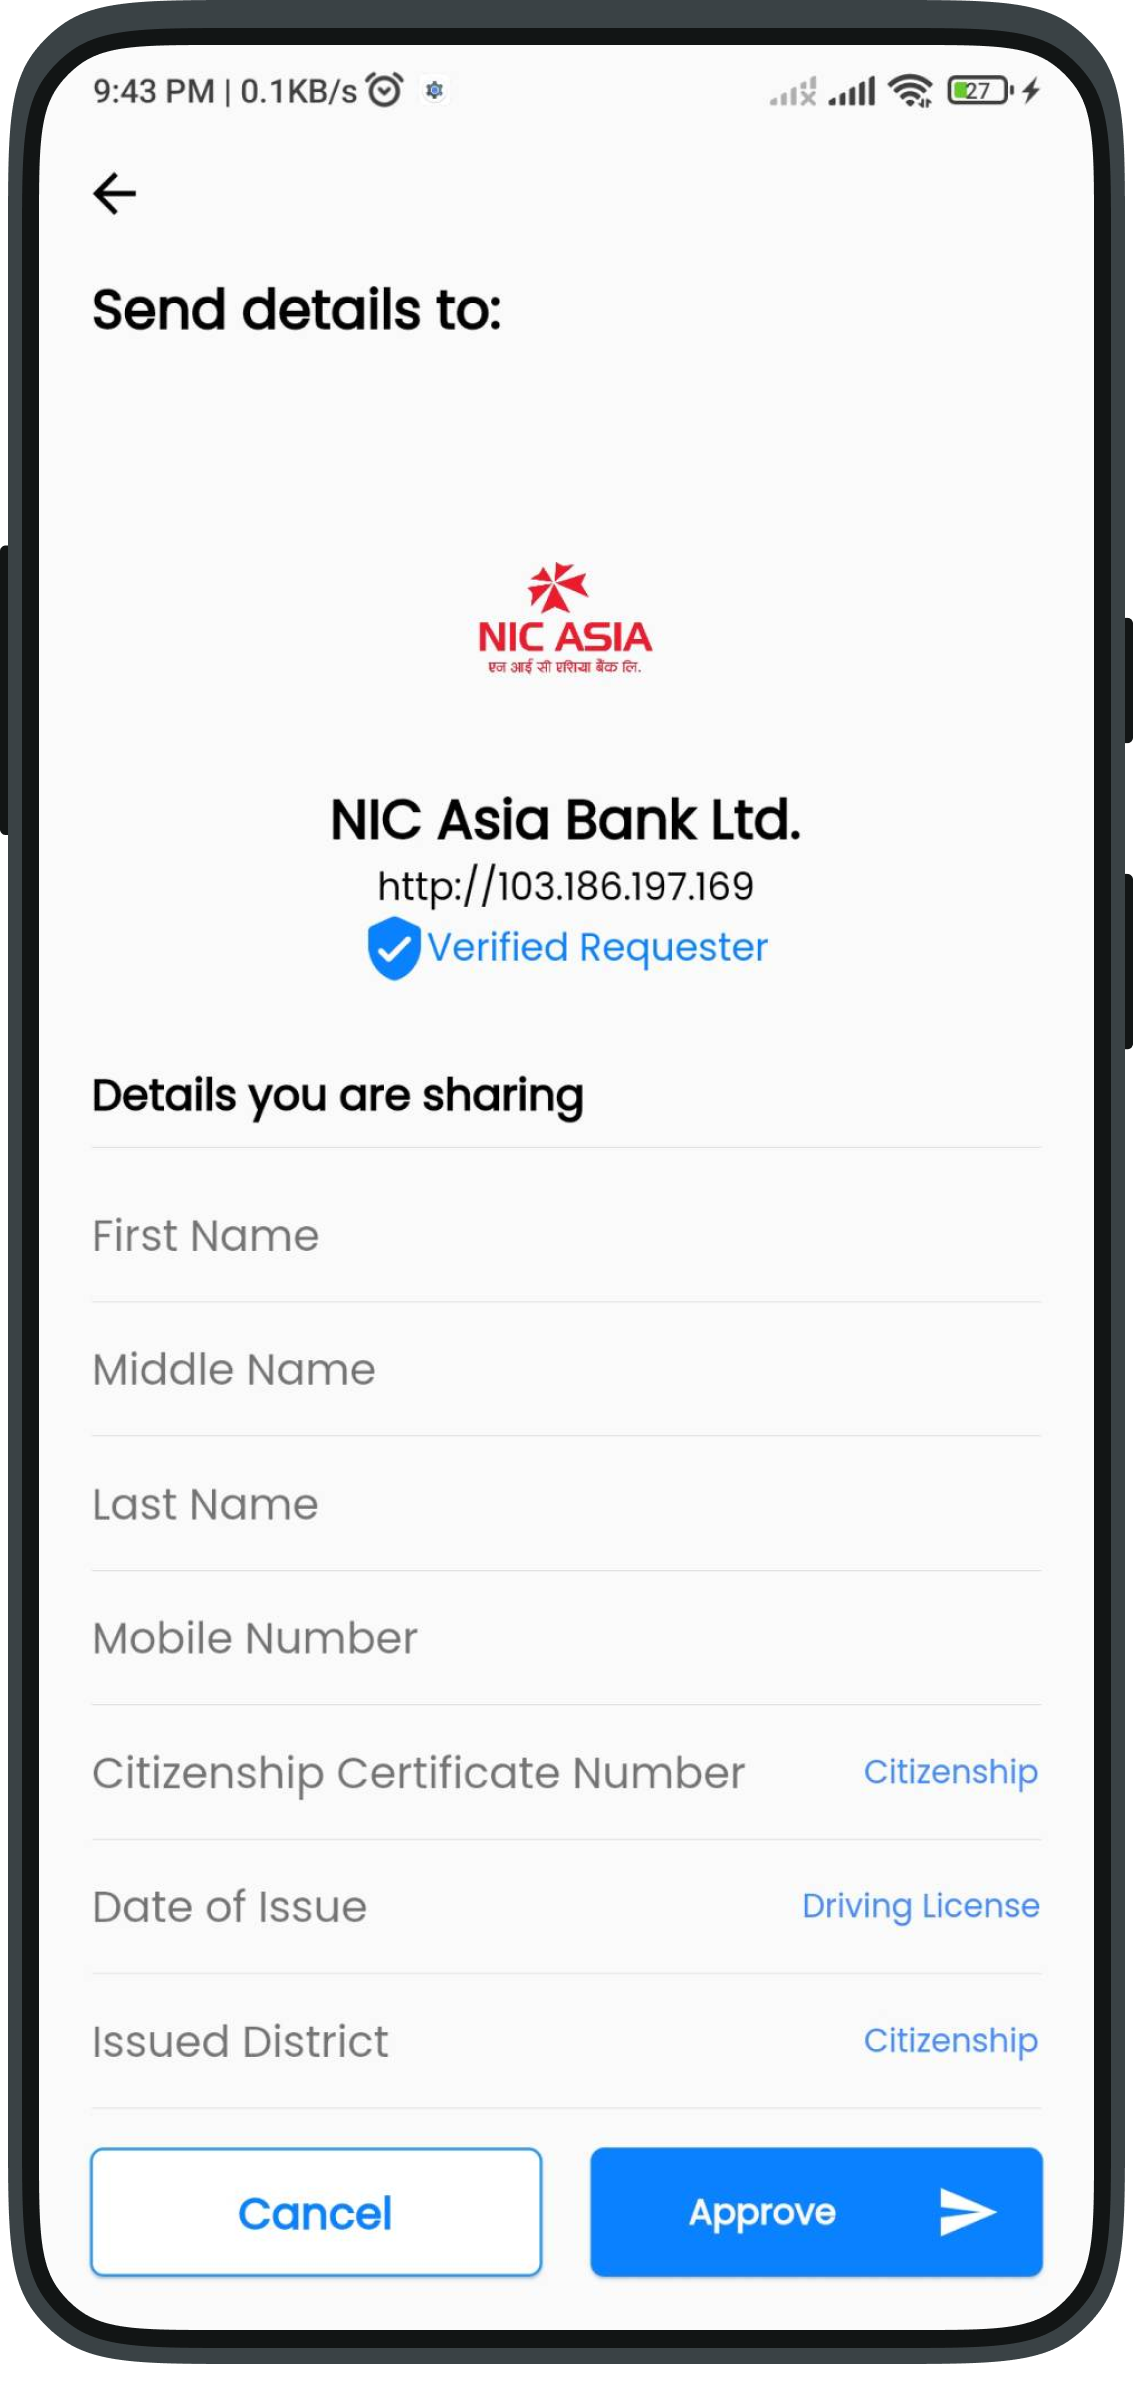
\includegraphics[width=0.3\linewidth]{images/results/mobile/DataAccessRequest.png}
            \caption[Access Request Permission Screen]{Access Request Permission Screen}
            \label{fig:DataAccessRequest.png}
            \end{figure}
        \textbf{Activity History}\\
        All of the user's activities, such as, logging into the device, generating QR codes to share details, scanning QR codes to obtain details, and much more are recorded and can be viewed in the history page. All the Shared or obtained details can be viewed by clicking on any of the history tile.
        \newpage
        \begin{multicols}{2}
            \begin{figure}[H]
            \centering
            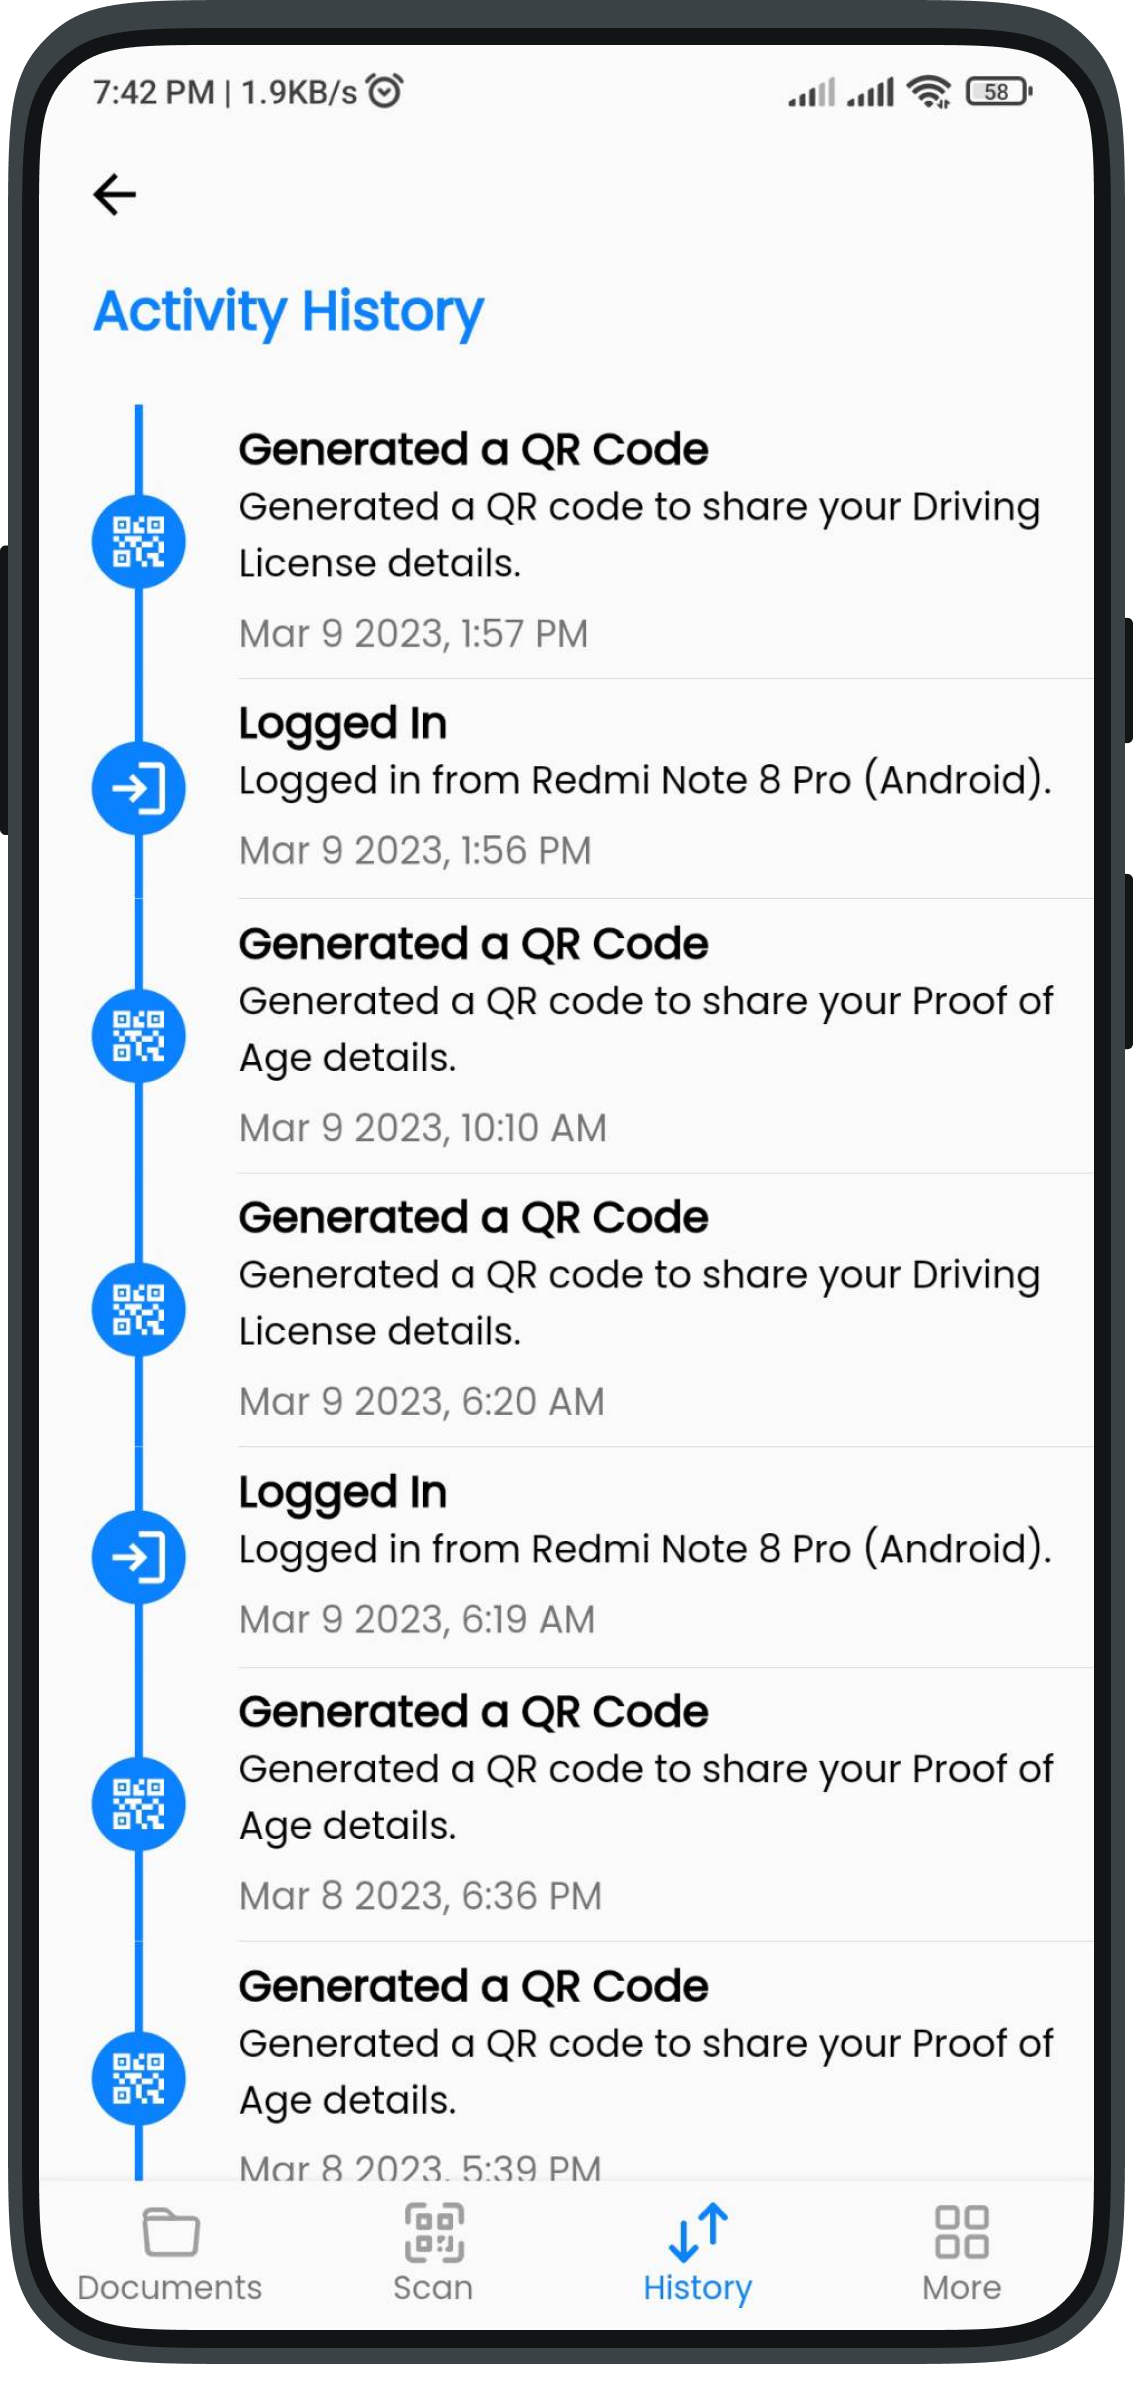
\includegraphics[width=0.6\linewidth]{images/results/mobile/History.png}
            \caption[Activity History Screen]{Activity History Screen}
            \label{fig:History.png}
            \end{figure} 

            \begin{figure}[H]
            \centering
            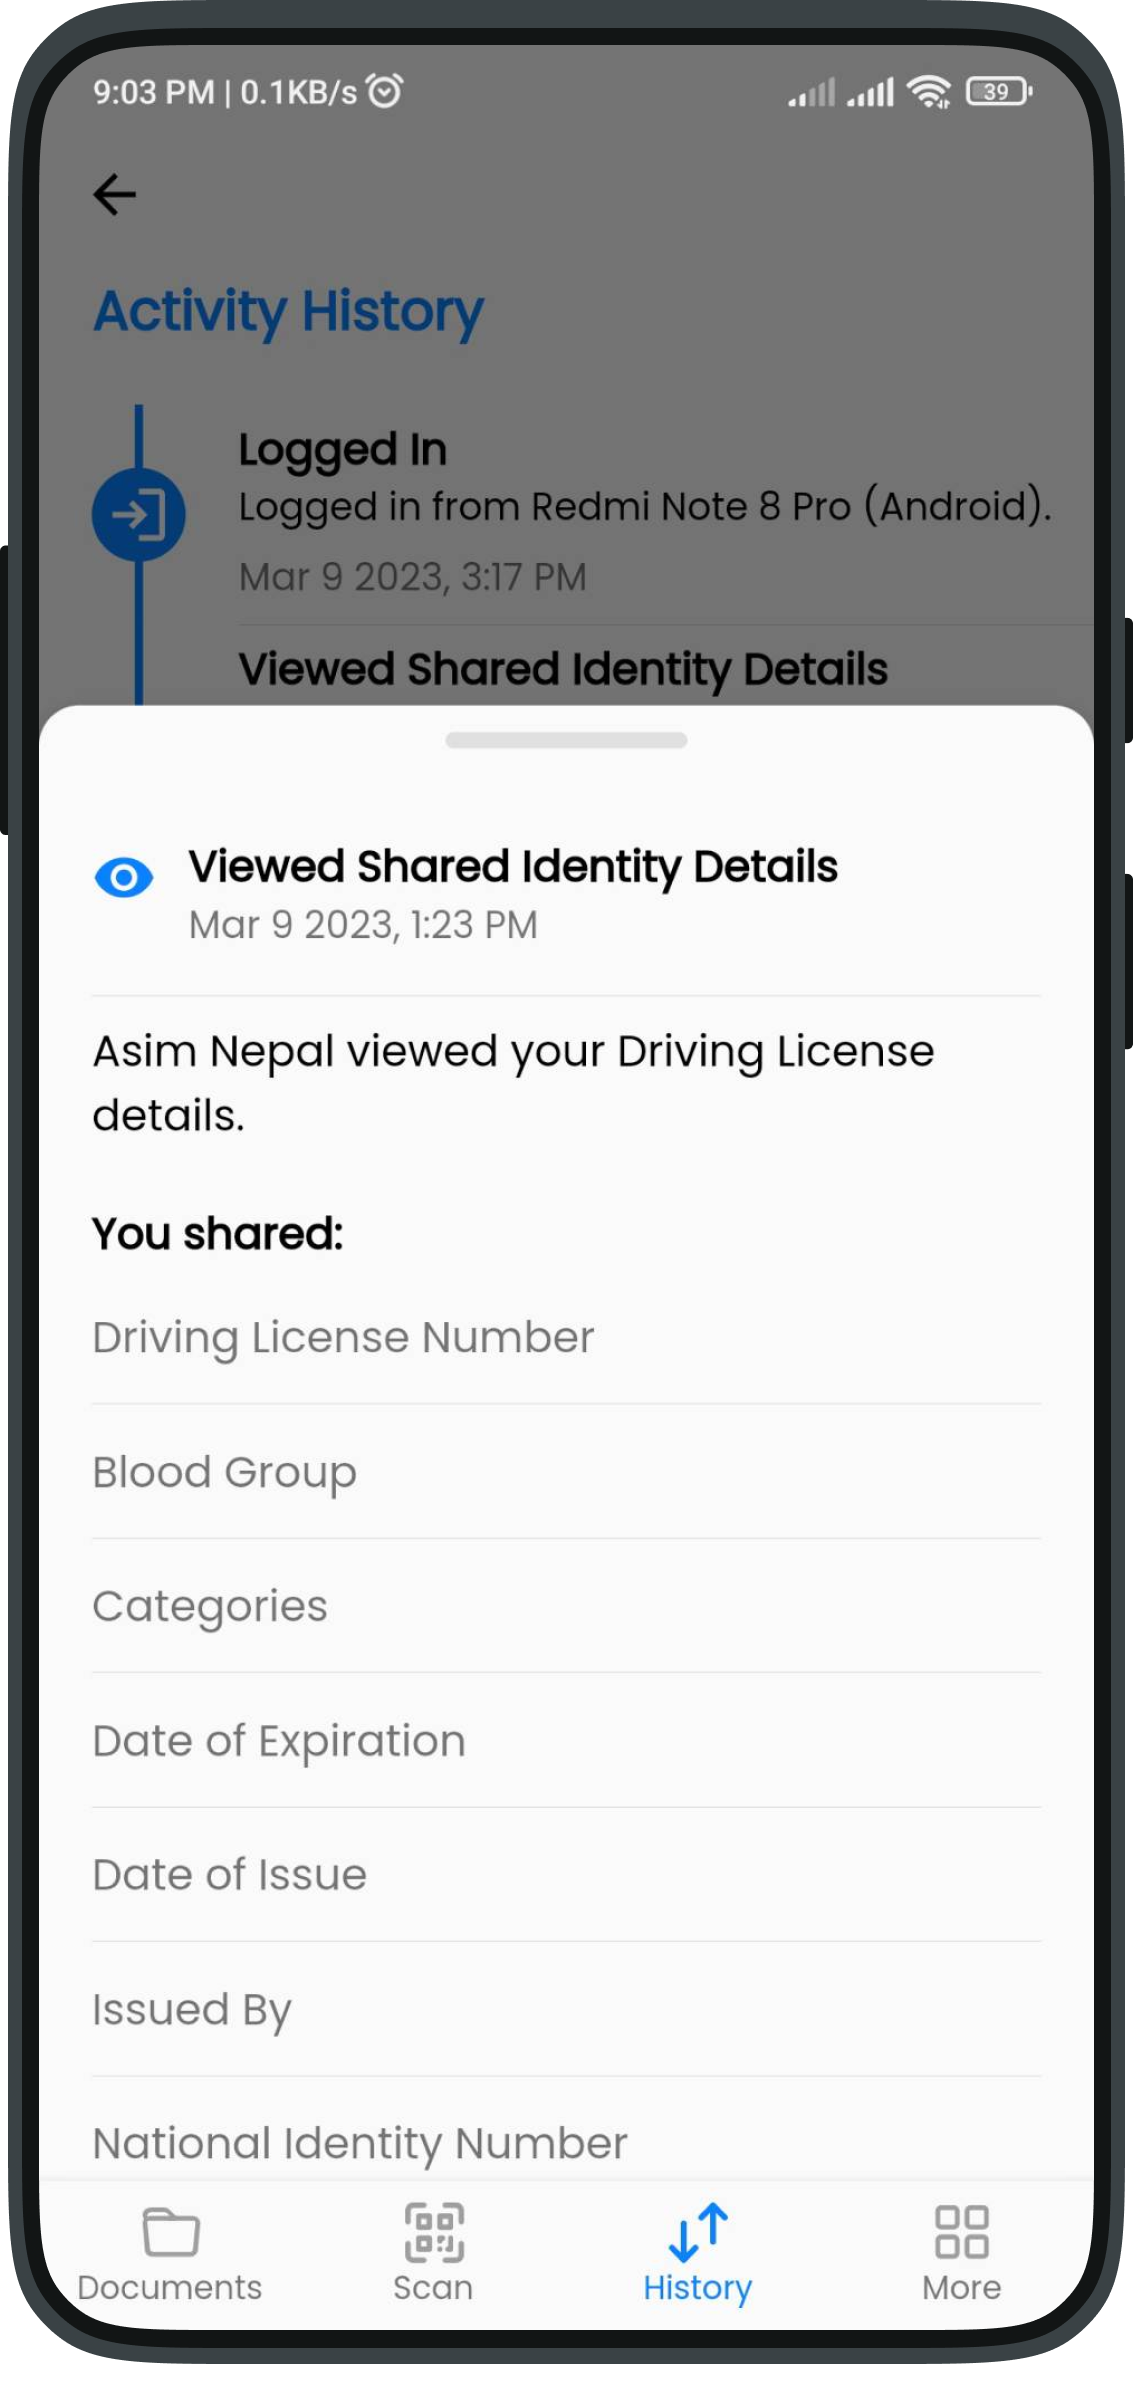
\includegraphics[width=0.6\linewidth]{images/results/mobile/HistoryDetails.png}
            \caption[History Log Details]{History Log Details}
            \label{fig:HistoryDetails.png}
            \end{figure}
        \end{multicols}
        
        \textbf{Other Features}\\
        Additional features and information of the app can be found in the more screen. Enabling or disabling dark mode, fingerprint to login, and logging out of the app are some of the features. 
        \begin{multicols}{2}
            \begin{figure}[H]
            \centering
            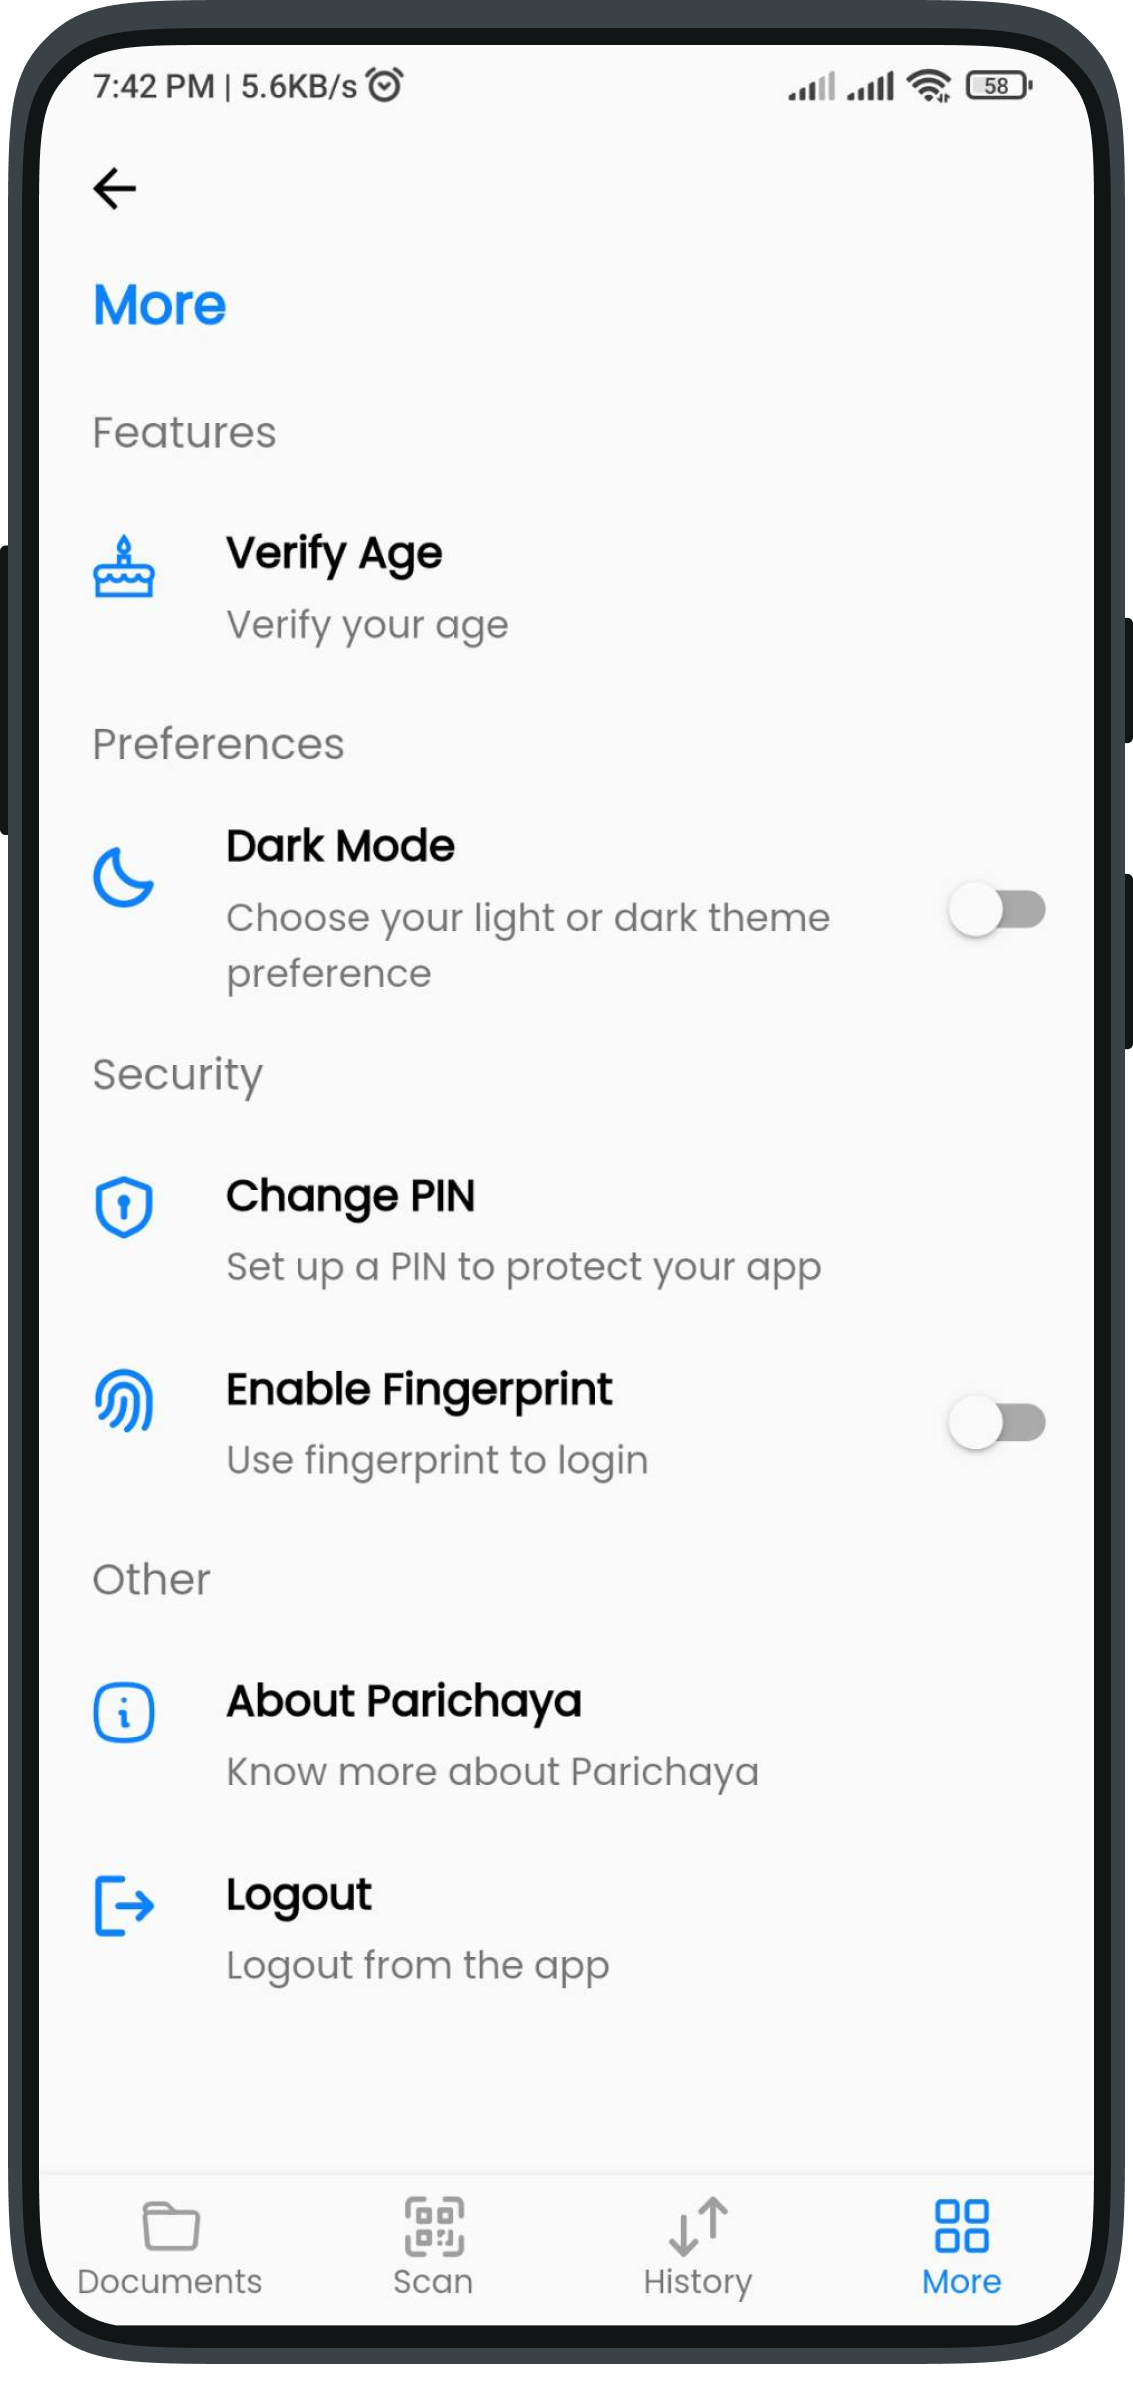
\includegraphics[width=0.6\linewidth]{images/results/mobile/More.png}
            \caption[More screen]{More Screen}
            \label{fig:More.png}
            \end{figure}     
            \begin{figure}[H]
            \centering
            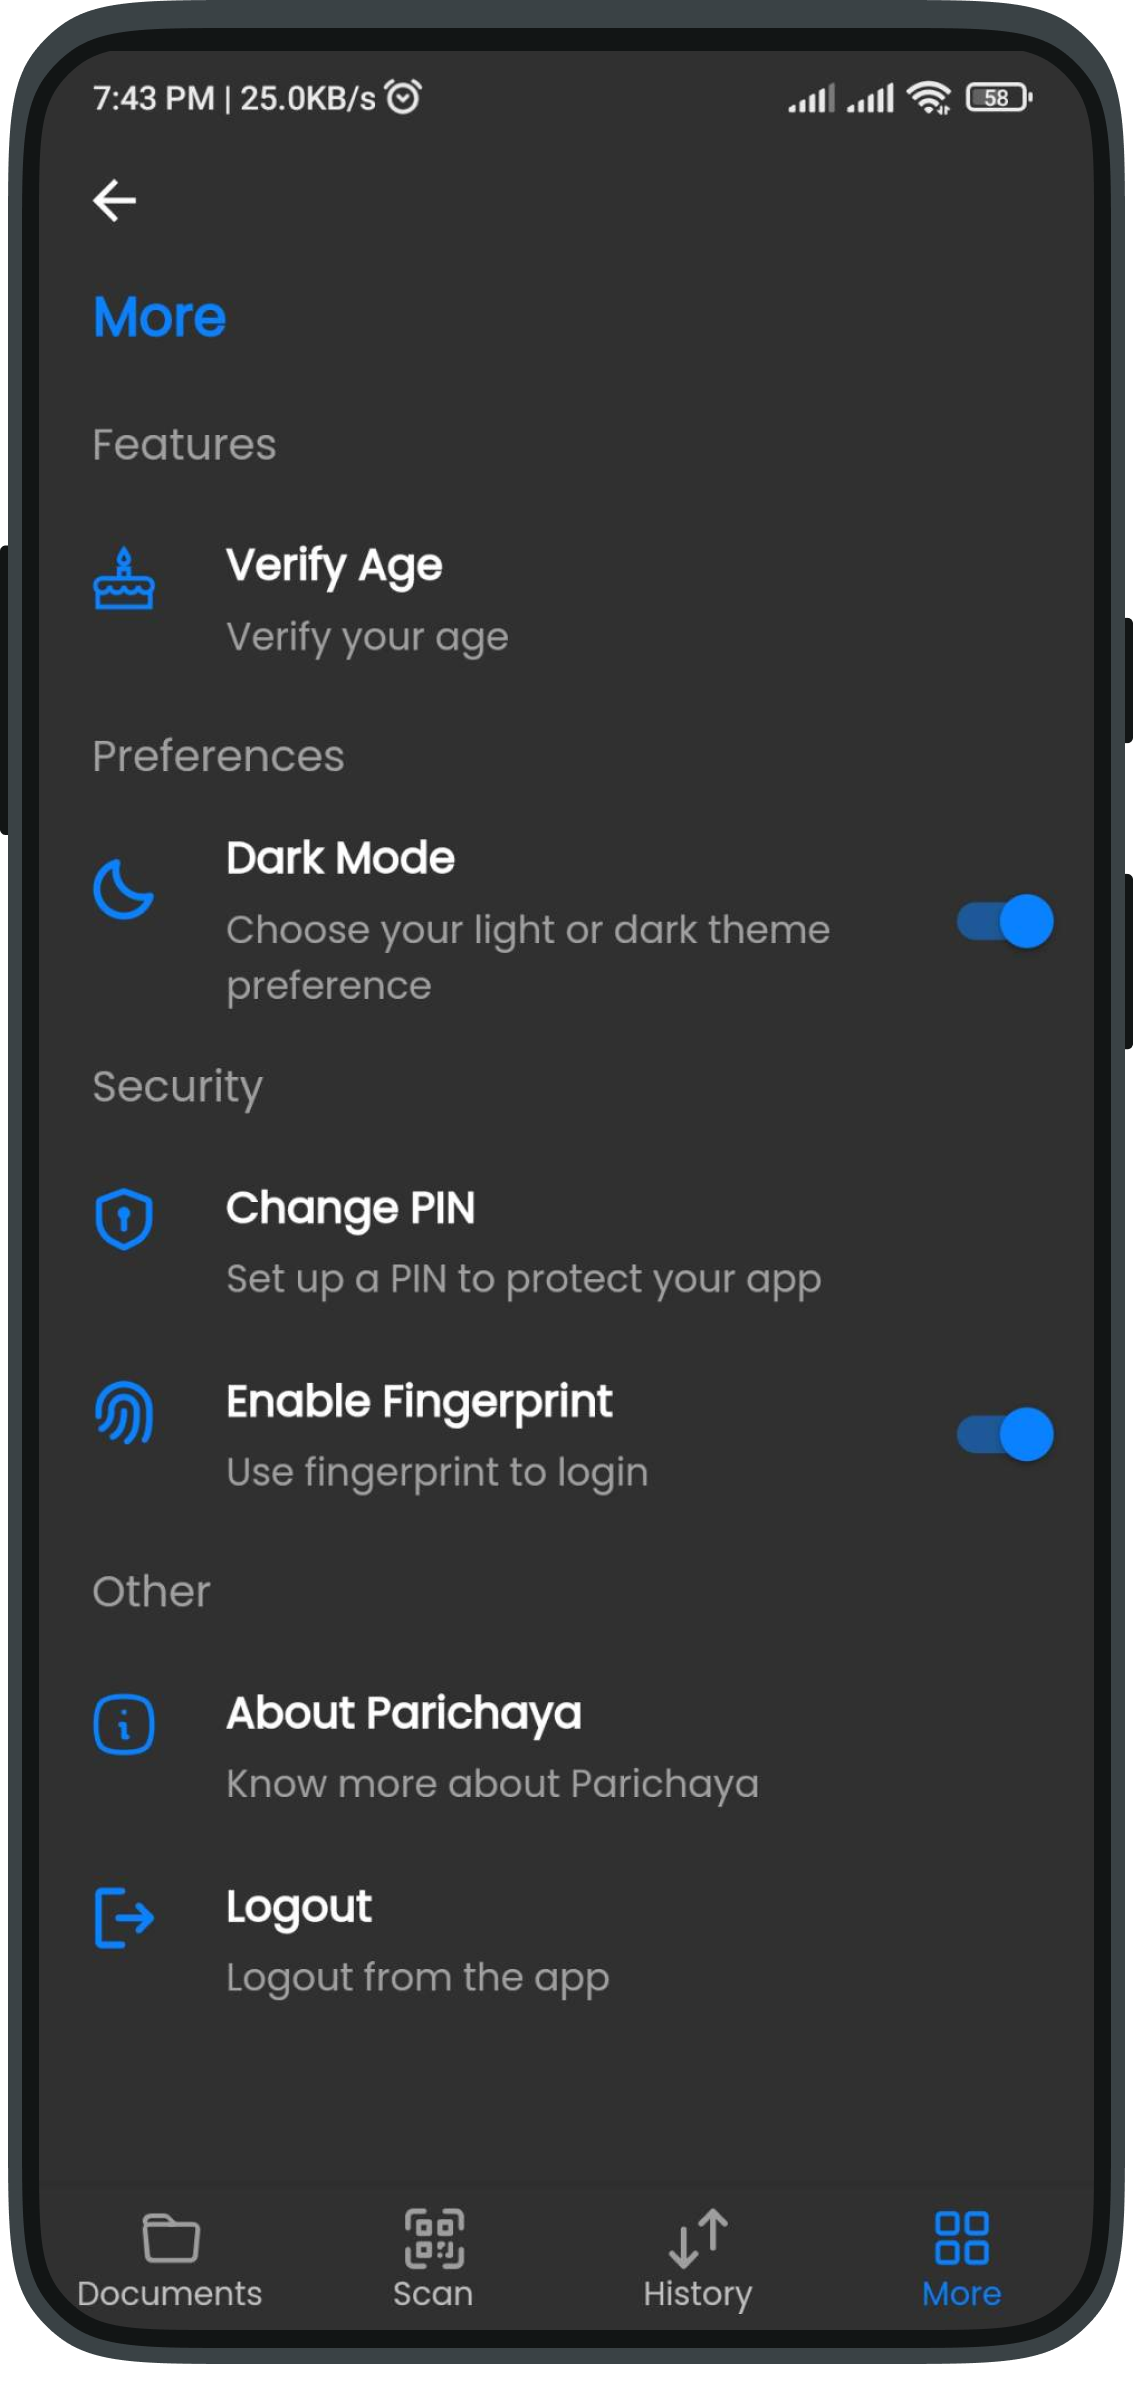
\includegraphics[width=0.6\linewidth]{images/results/mobile/MoreDarkMode.png}
            \caption[More Screen in Dark mode]{More Screen in Dark mode} 
            \label{fig:MoreDarkMode.png}
            \end{figure}
           \end{multicols}

           \textbf{Change MPIN}\\
           User can change their mpin when they are logged in either by scanning their fingerprint or by entering their previous mpin.
           
        \begin{multicols}{2}
            \begin{figure}[H]
            \centering
            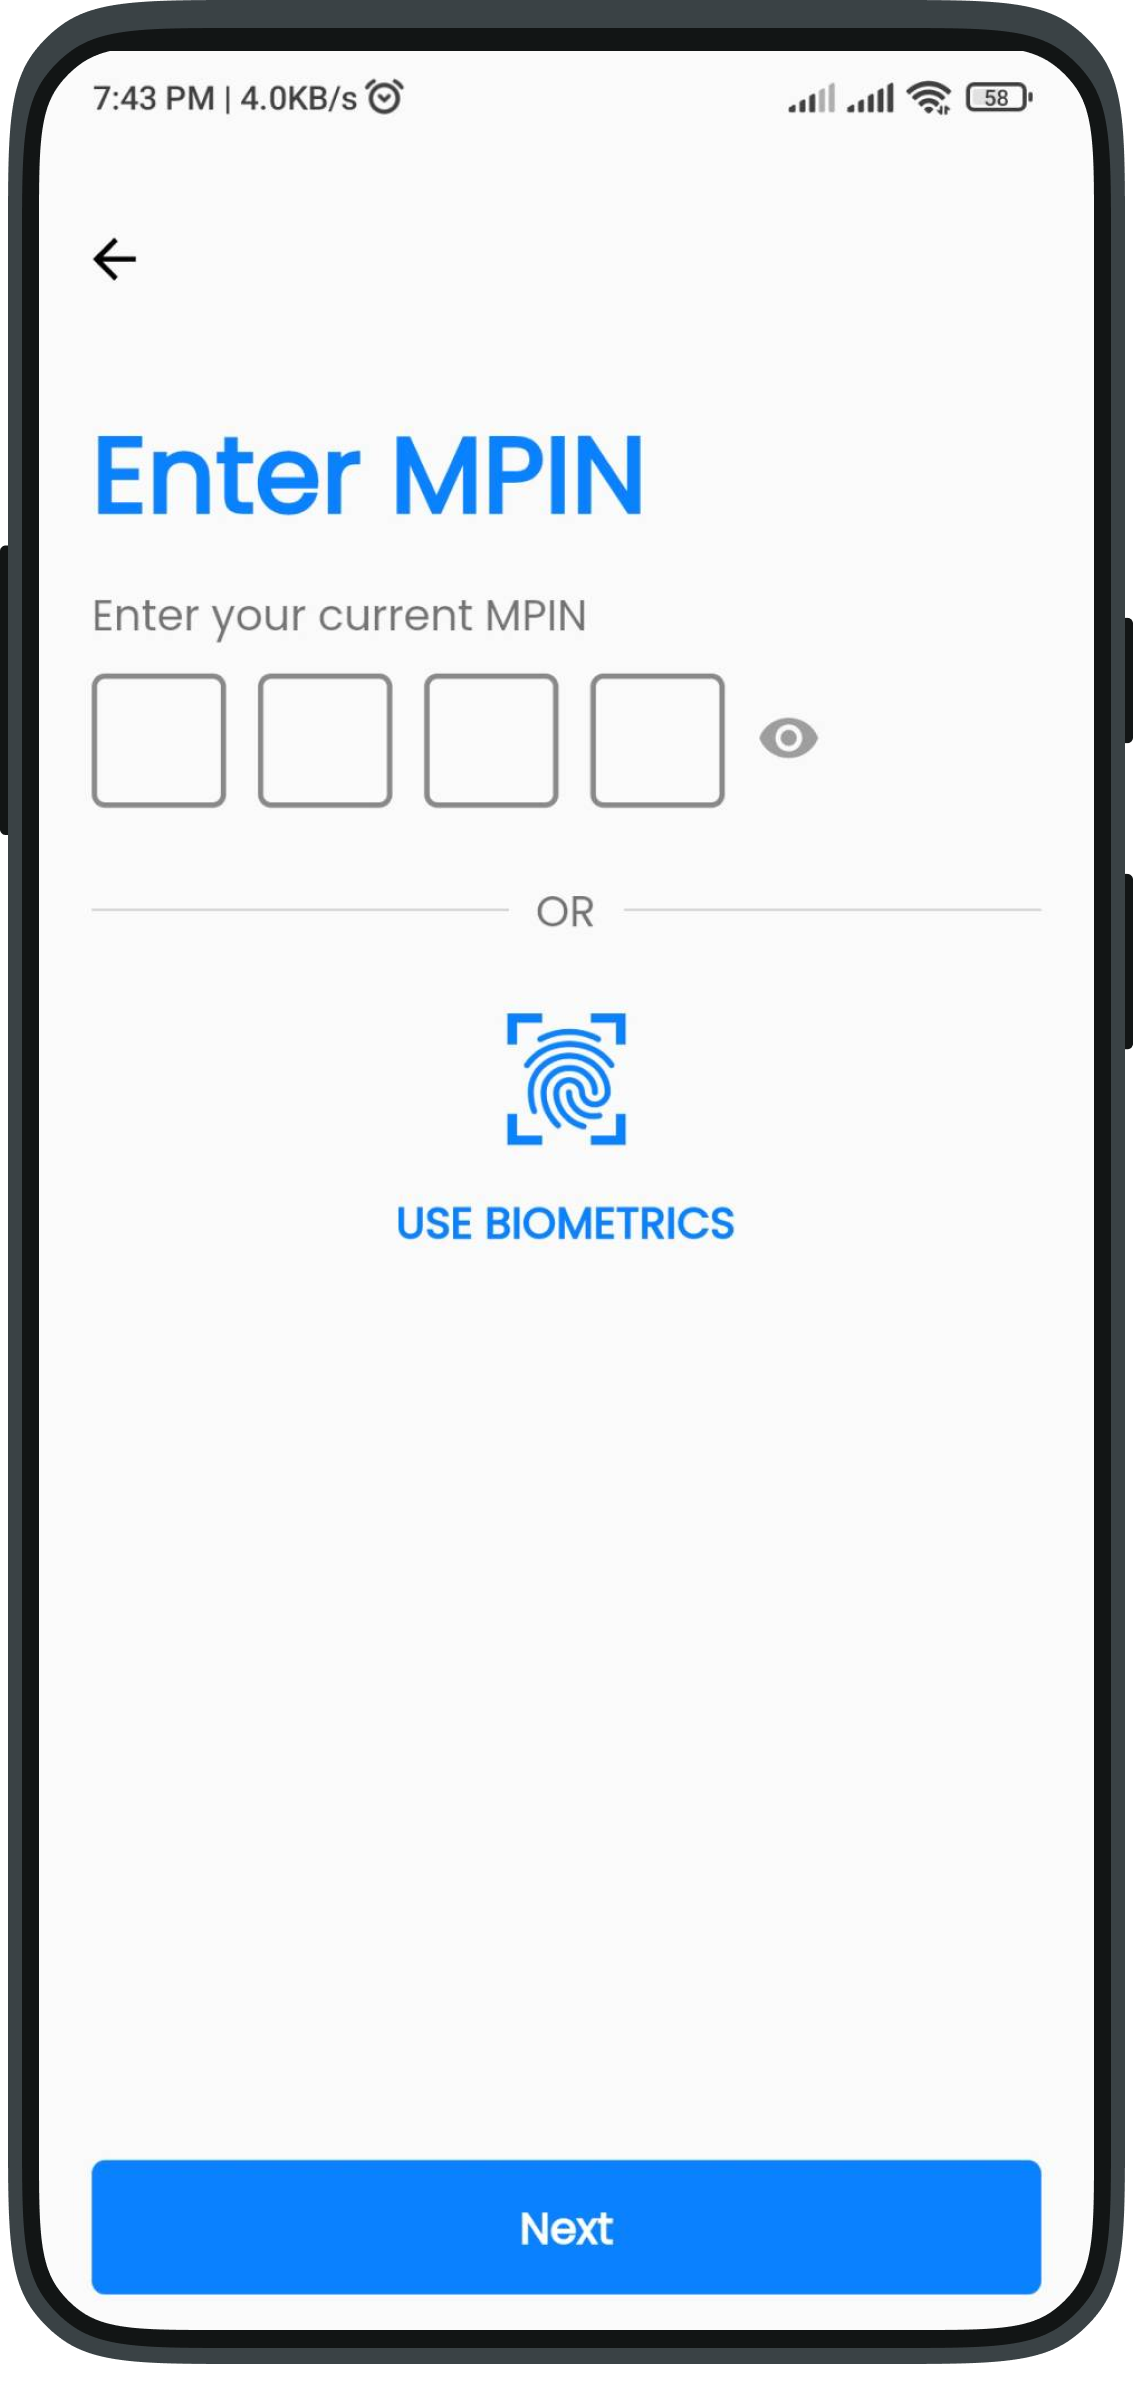
\includegraphics[width=0.6\linewidth]{images/results/mobile/ChangeMPIN.png}
            \caption[Enter Old MPIN Screen]{Enter Old MPIN Screen}
            \label{fig:ChangeMPIN.png}
            \end{figure}
            \begin{figure}[H]
            \centering
            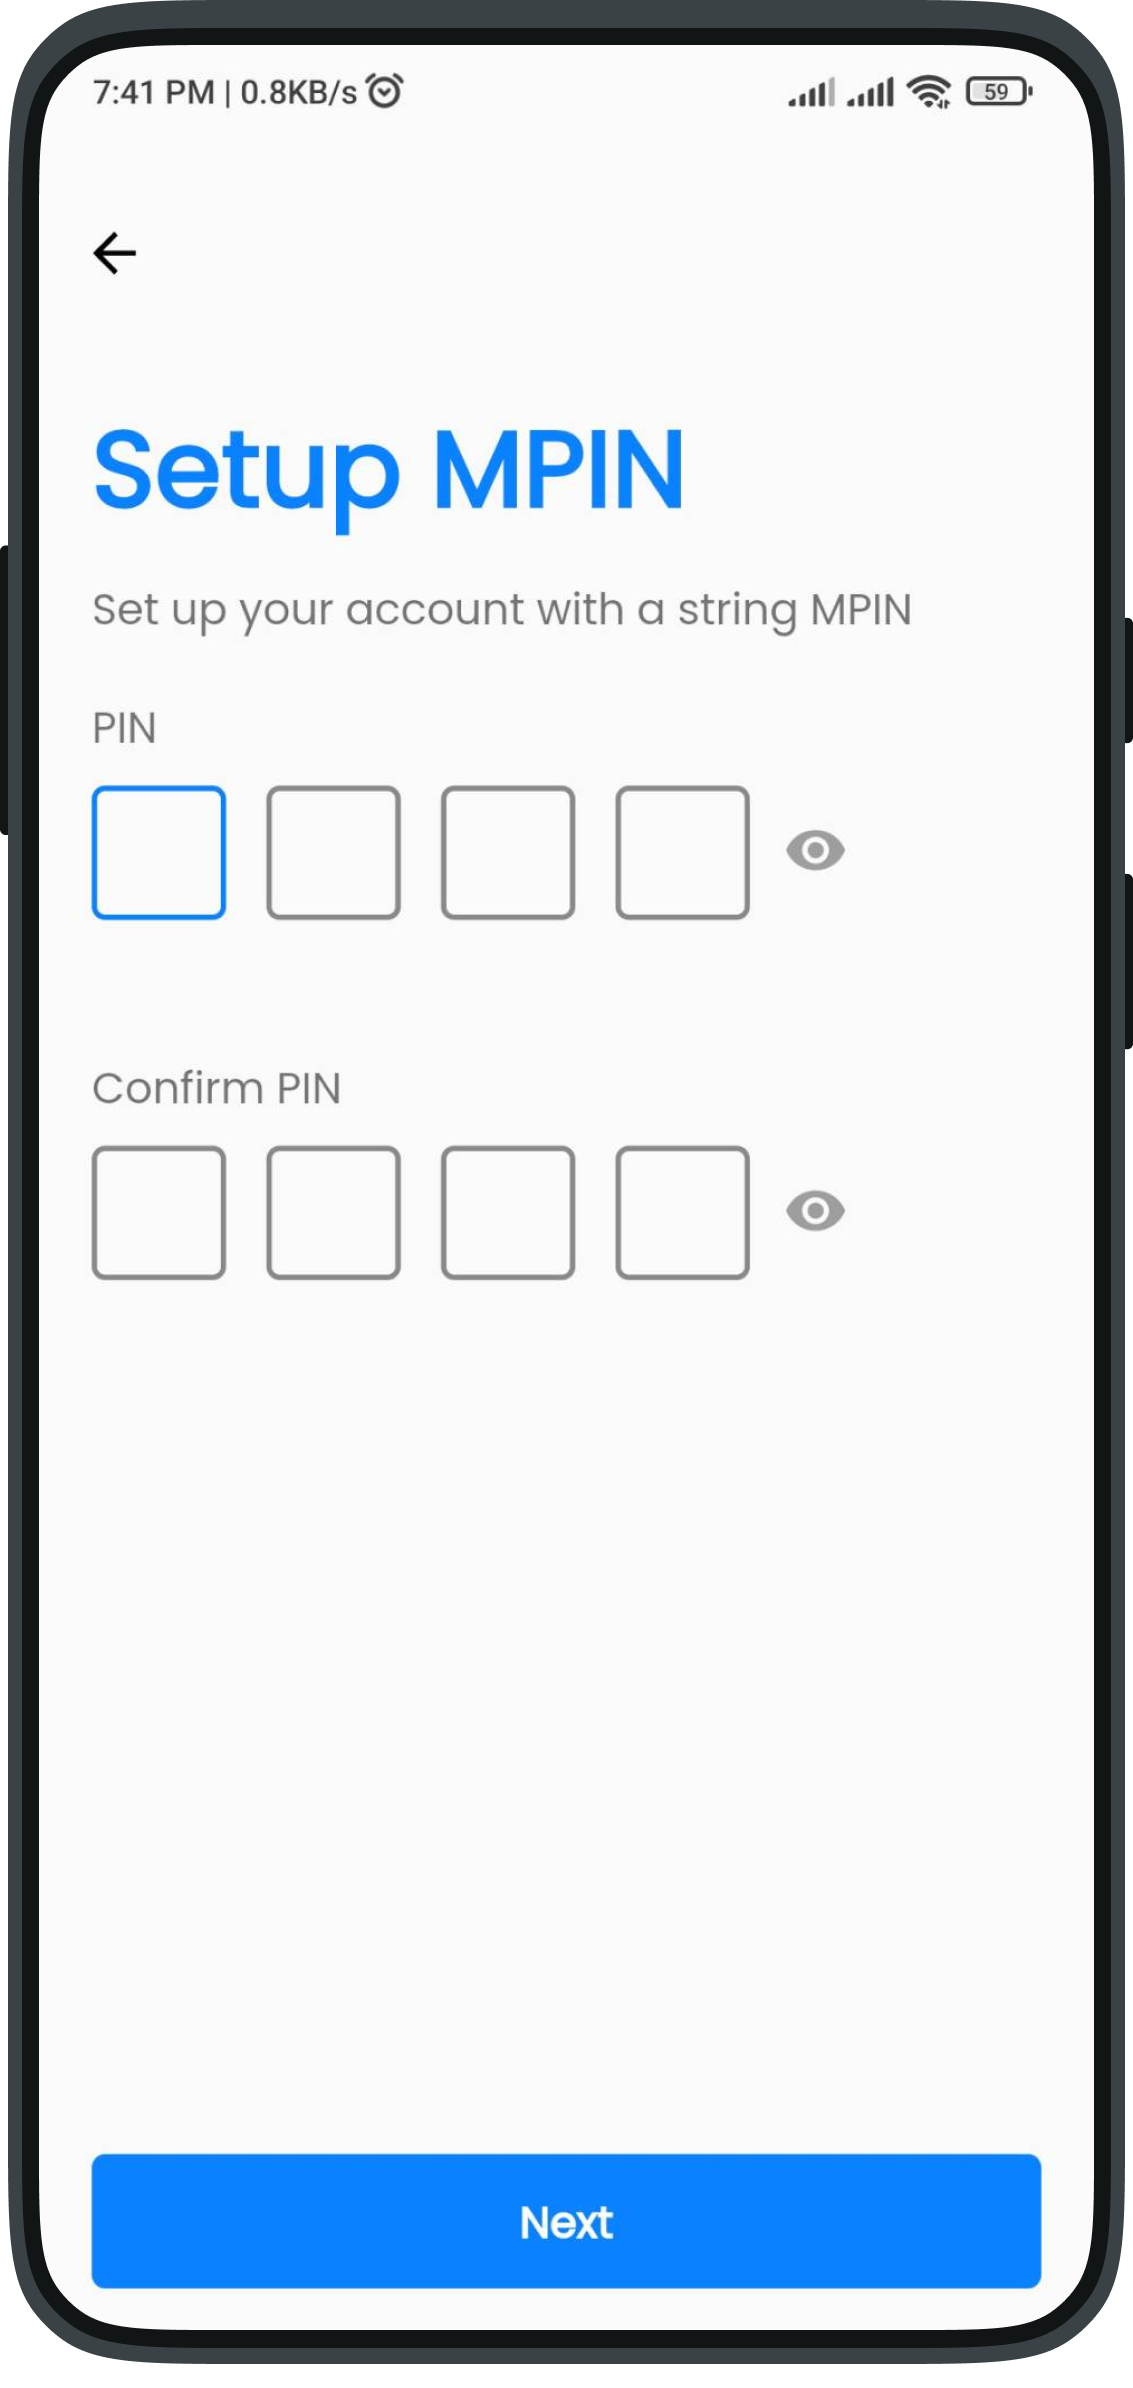
\includegraphics[width=0.6\linewidth]{images/results/mobile/SetupMPIN.png}
            \caption[Enter New MPIN Screen]{Enter New MPIN Screen}
            \label{fig:SetupMPIN.png}
            \end{figure}
        \end{multicols}

        \textbf{About Us}\\
         Users can learn more about the app and the developers who made it in the about us page. Users may view all the open source licenses that were used in the development of the app. Users may also gain knowledge about the developers by reading the team overview.
         \newpage
         \begin{multicols}{3}
            \begin{figure}[H]
            \centering
            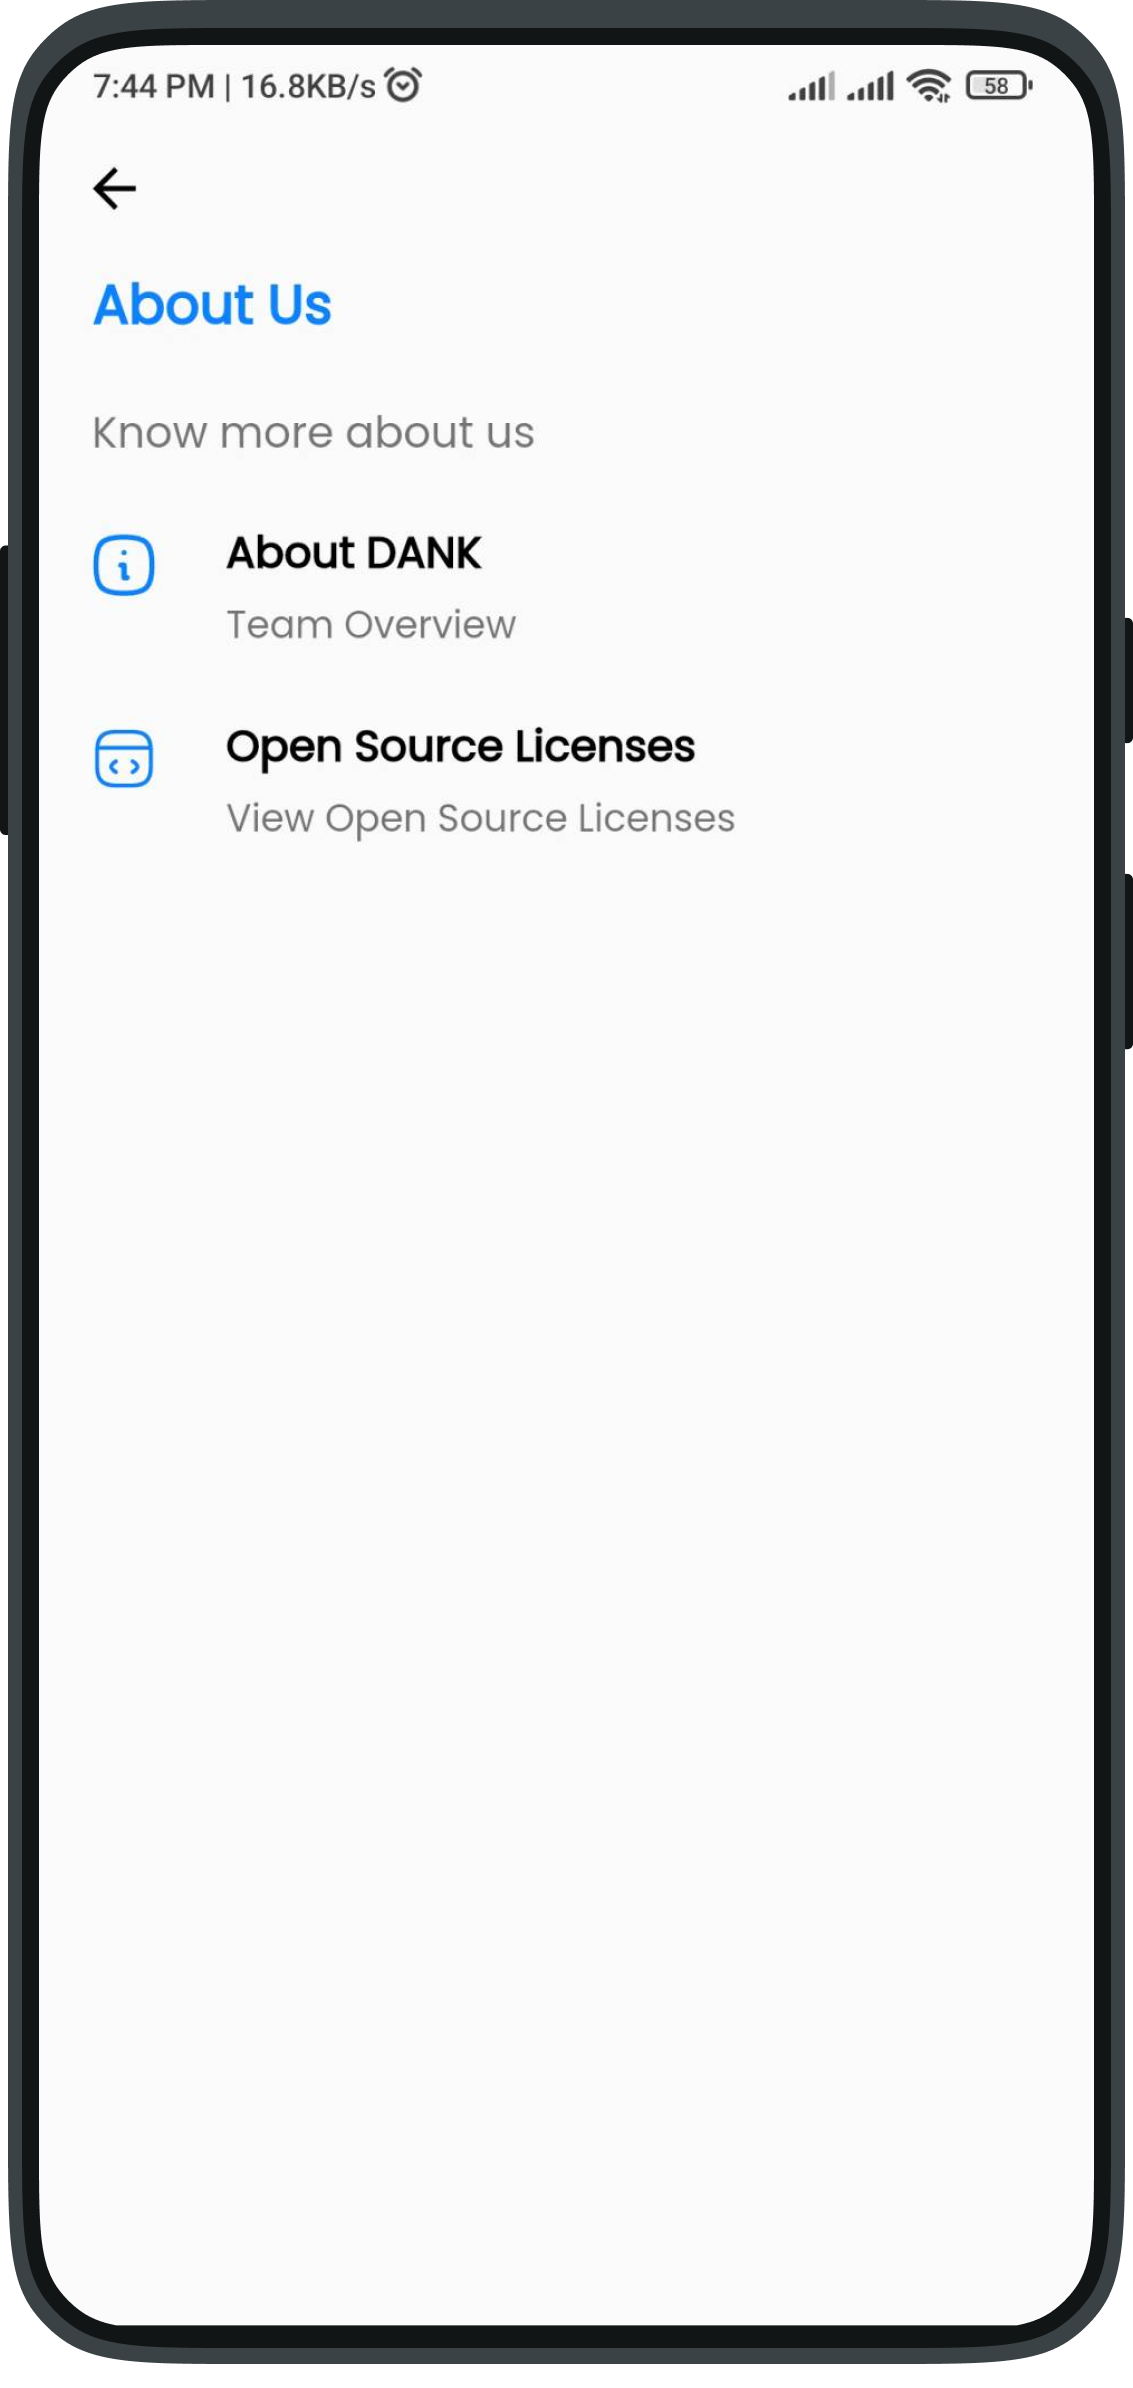
\includegraphics[width=0.85\linewidth]{images/results/mobile/AboutUs.png}
            \caption[About Us]{About Us}
            \label{fig:AboutUs.png}
            \end{figure}     
            \begin{figure}[H]
            \centering
            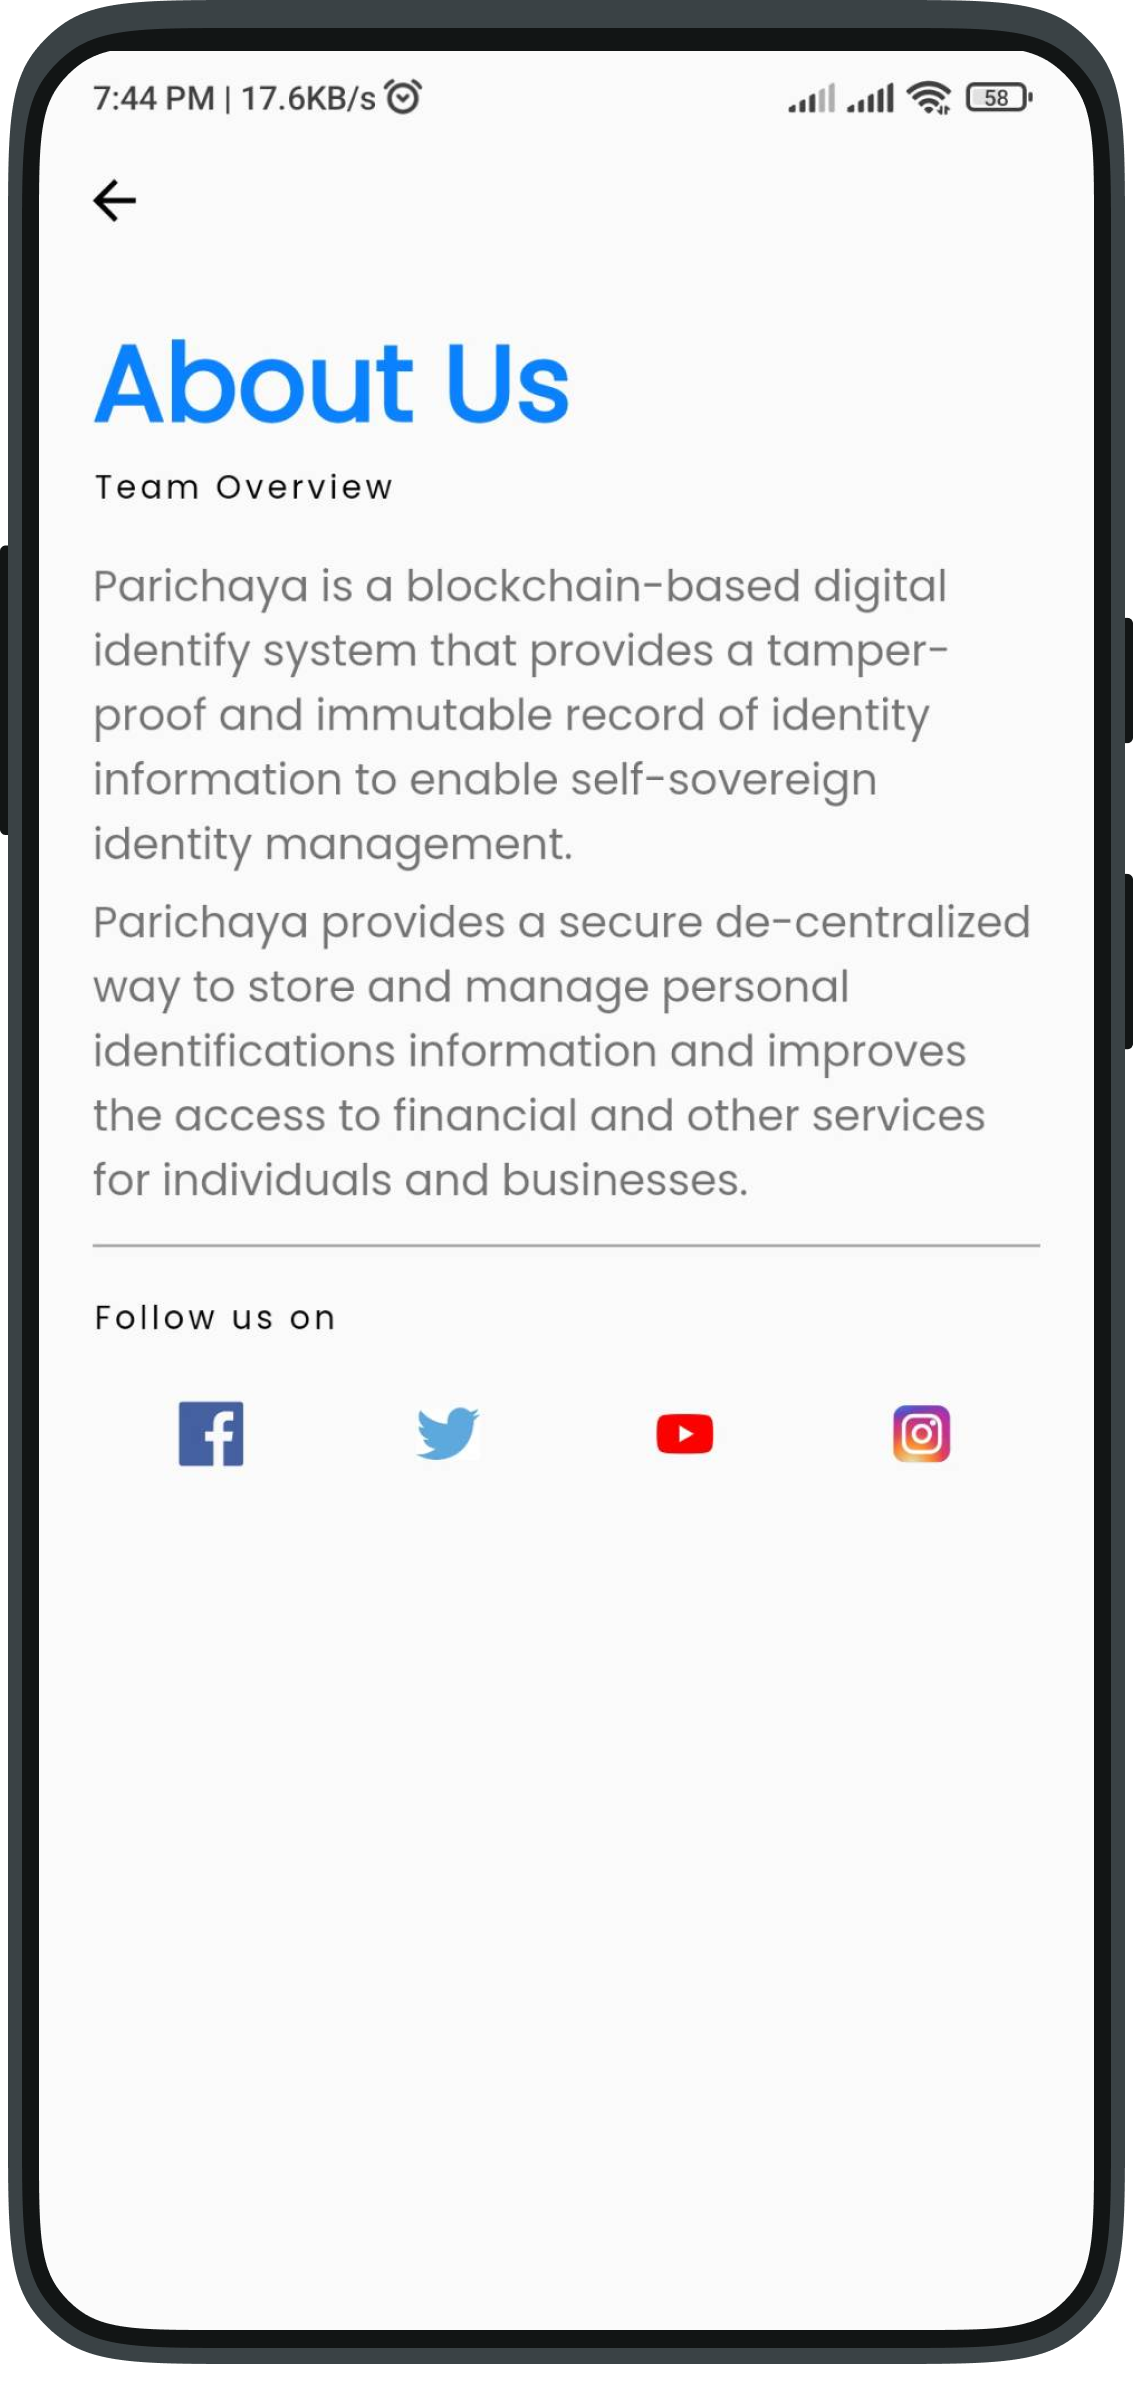
\includegraphics[width=0.85\linewidth]{images/results/mobile/TeamOverview.png}
            \caption[About Dank]{About Dank}
            \label{fig:TeamOverview.png}
            \end{figure}
            \begin{figure}[H]
            \centering
            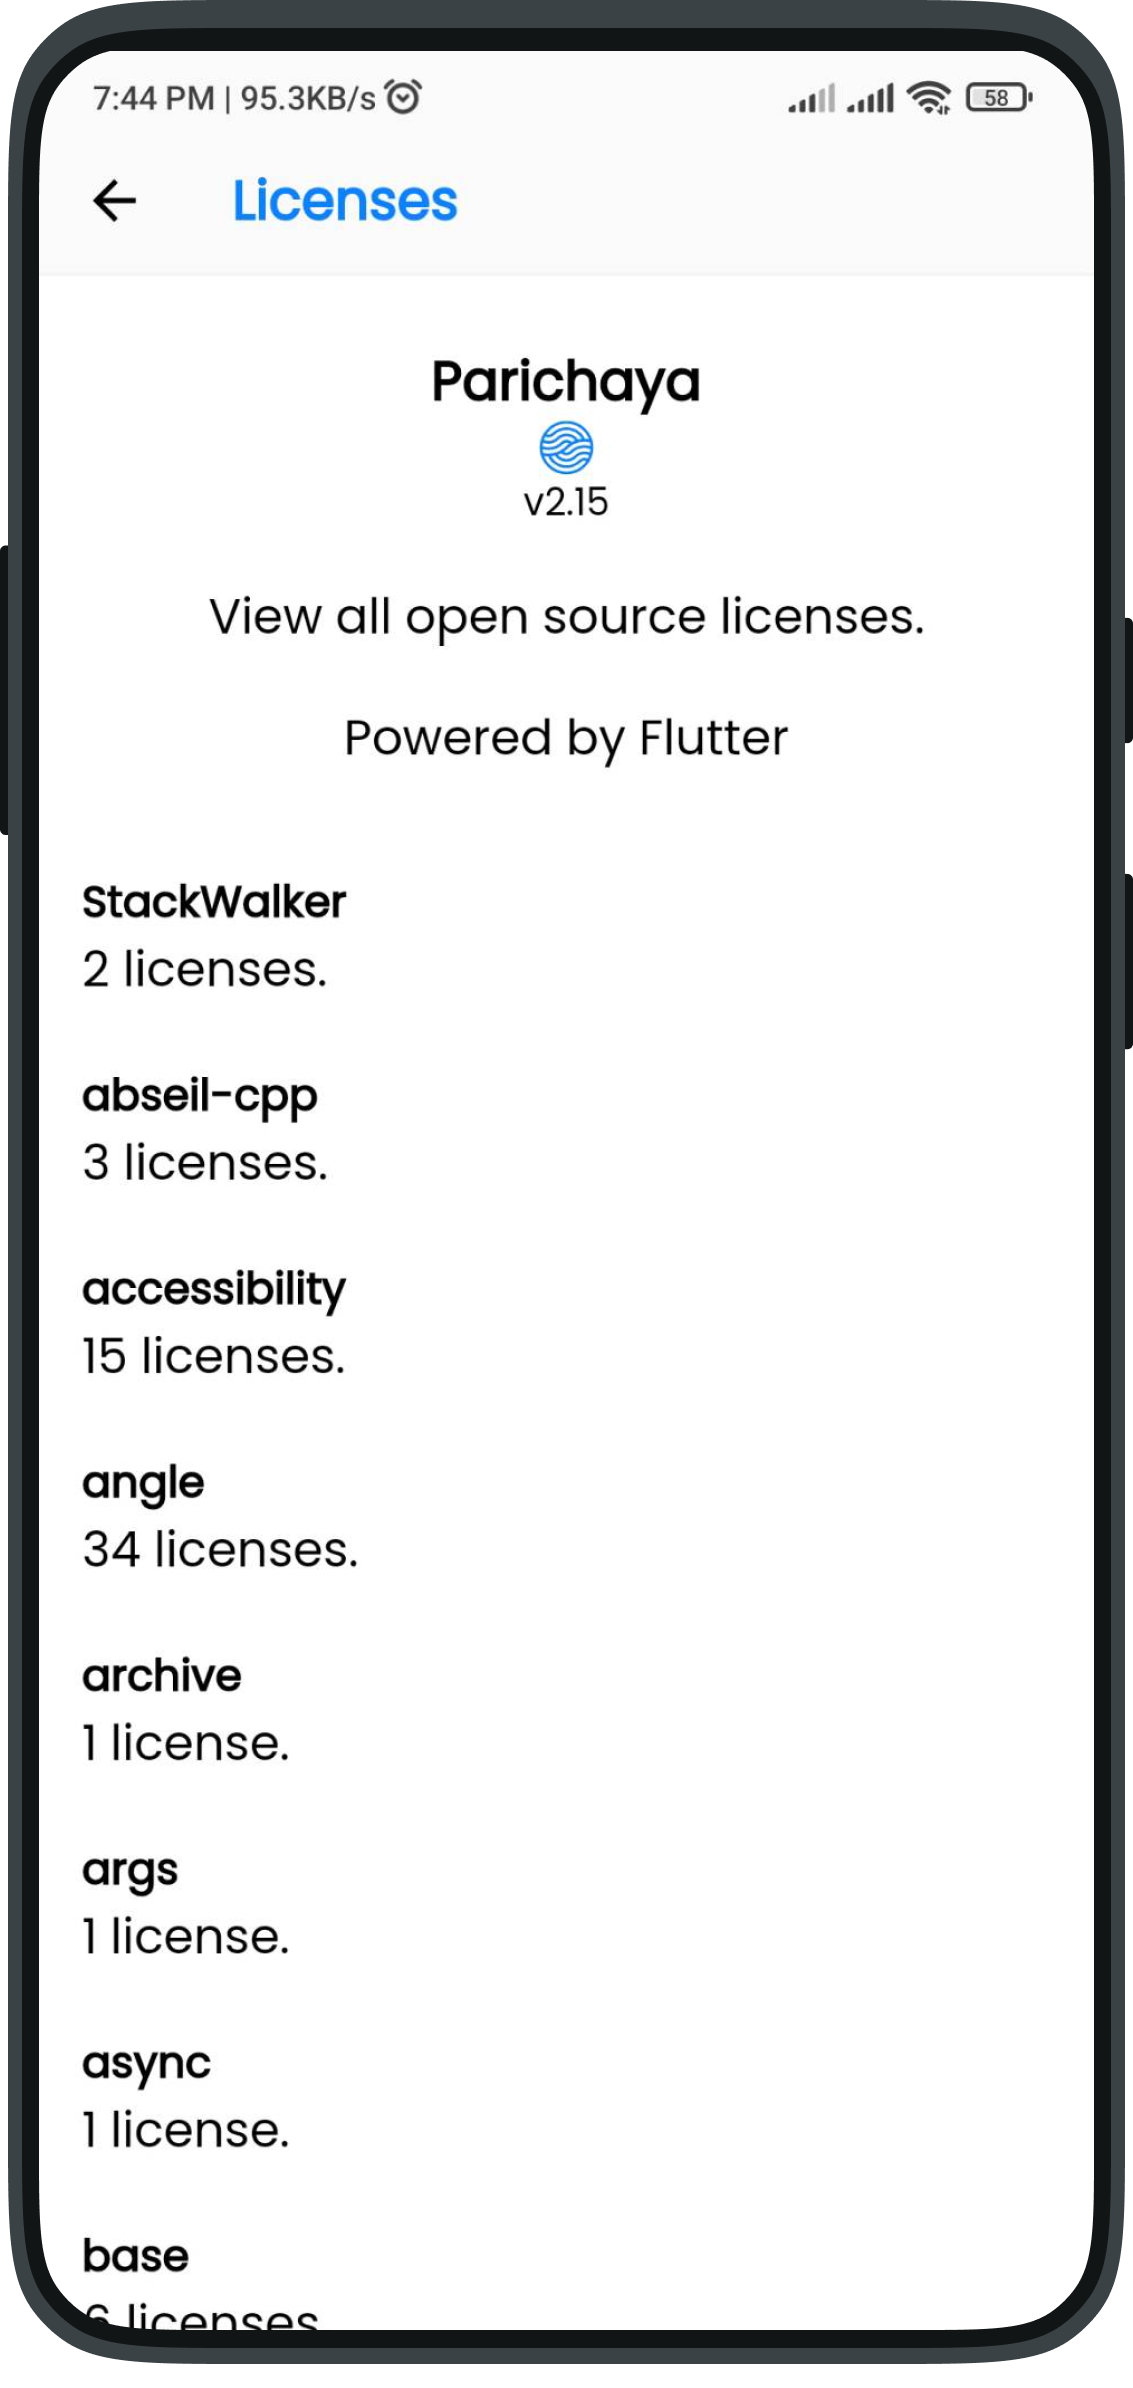
\includegraphics[width=0.85\linewidth]{images/results/mobile/OpenSourceLicenses.png}
            \caption[License]{License}
            \label{fig:OpenSourceLicenses.png}
            \end{figure}
        
        \end{multicols}

        \textbf{Log Out}\\
        When user log outs of the application.
         \begin{figure}[H]
            \centering
            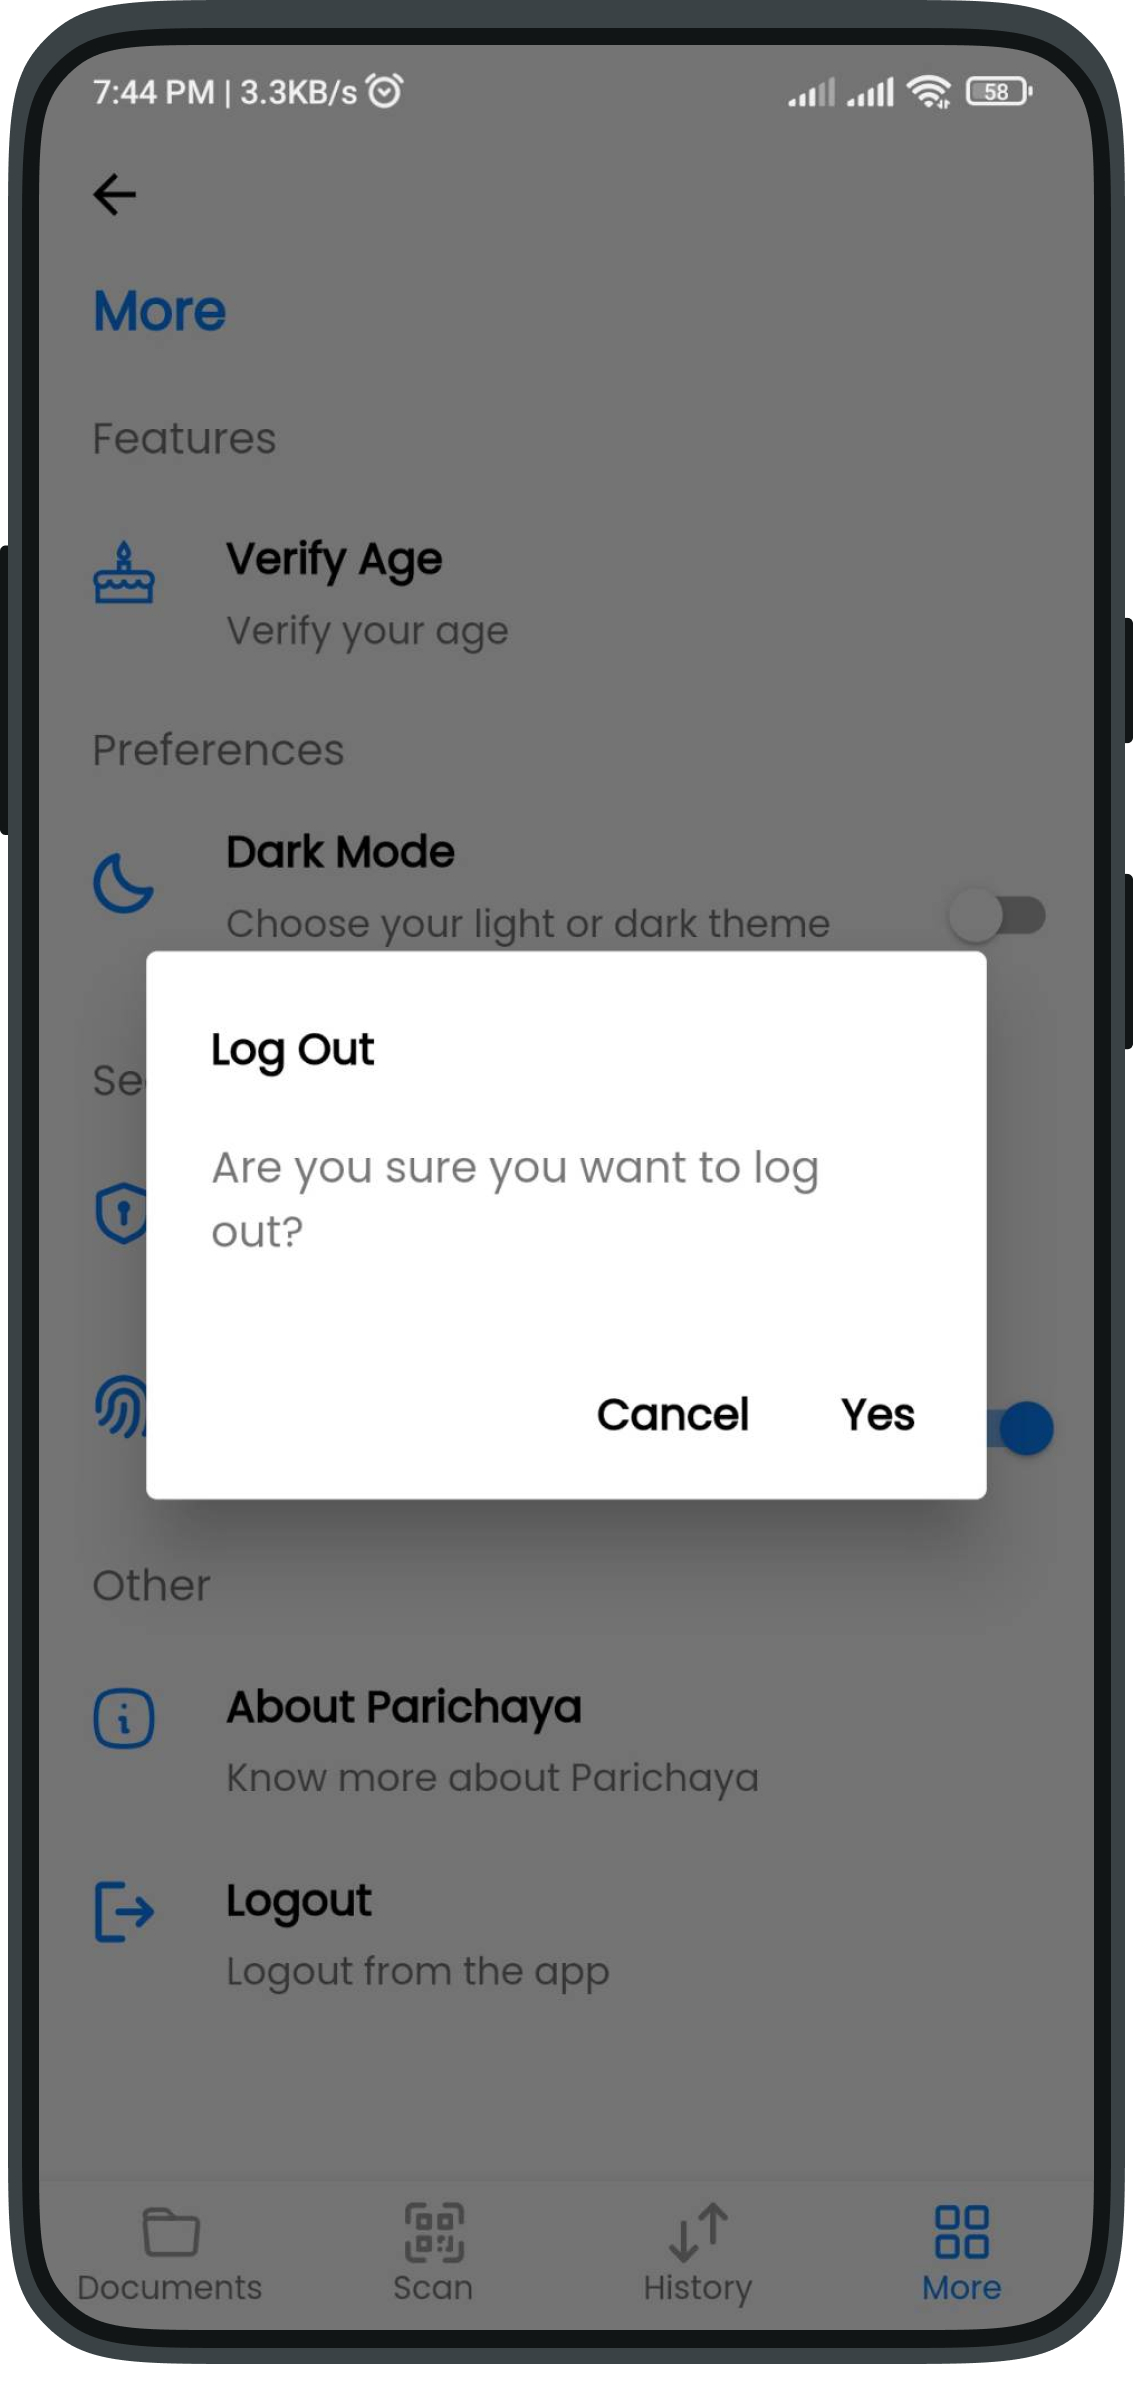
\includegraphics[width=0.3\linewidth]{images/results/mobile/Logout.png}
            \caption[Logout]{Logout}
            \label{fig:Logout.png}
            \end{figure}

       
     
\subsection{Website Application}
  Employee of government working on issuing national identity, citizenship and driving license who is register in database can log in to the portal by giving correct username and their password.

        \begin{figure}[H]
        \centering
        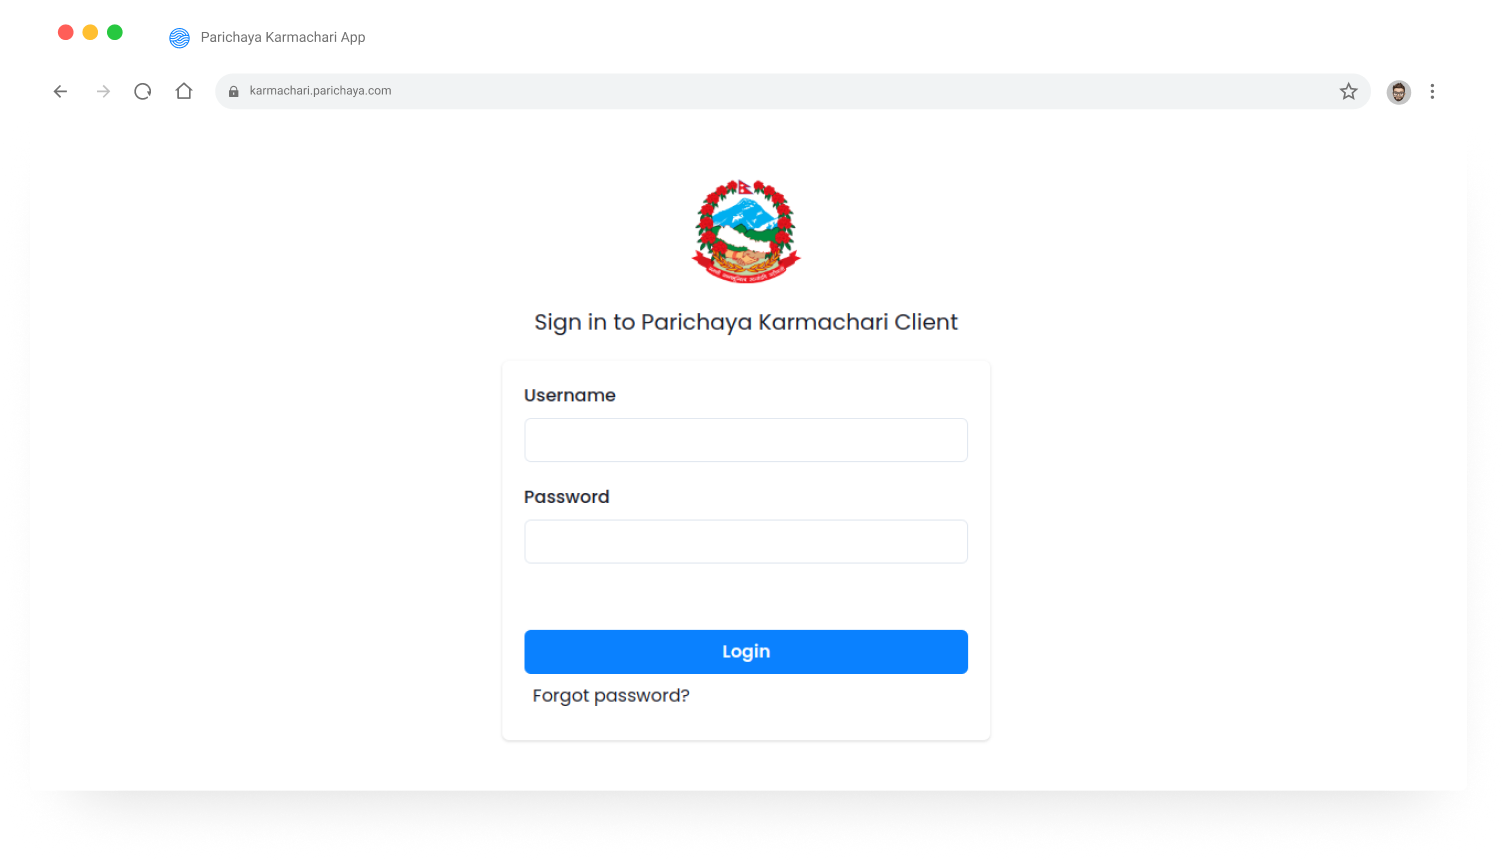
\includegraphics[width=0.6\linewidth]{images/results/web/WebLoginPage.png}
        \caption[Login]{Login}
        \label{fig:WebLoginPage.png}
        \end{figure}

           \begin{figure}[H]
        \centering
        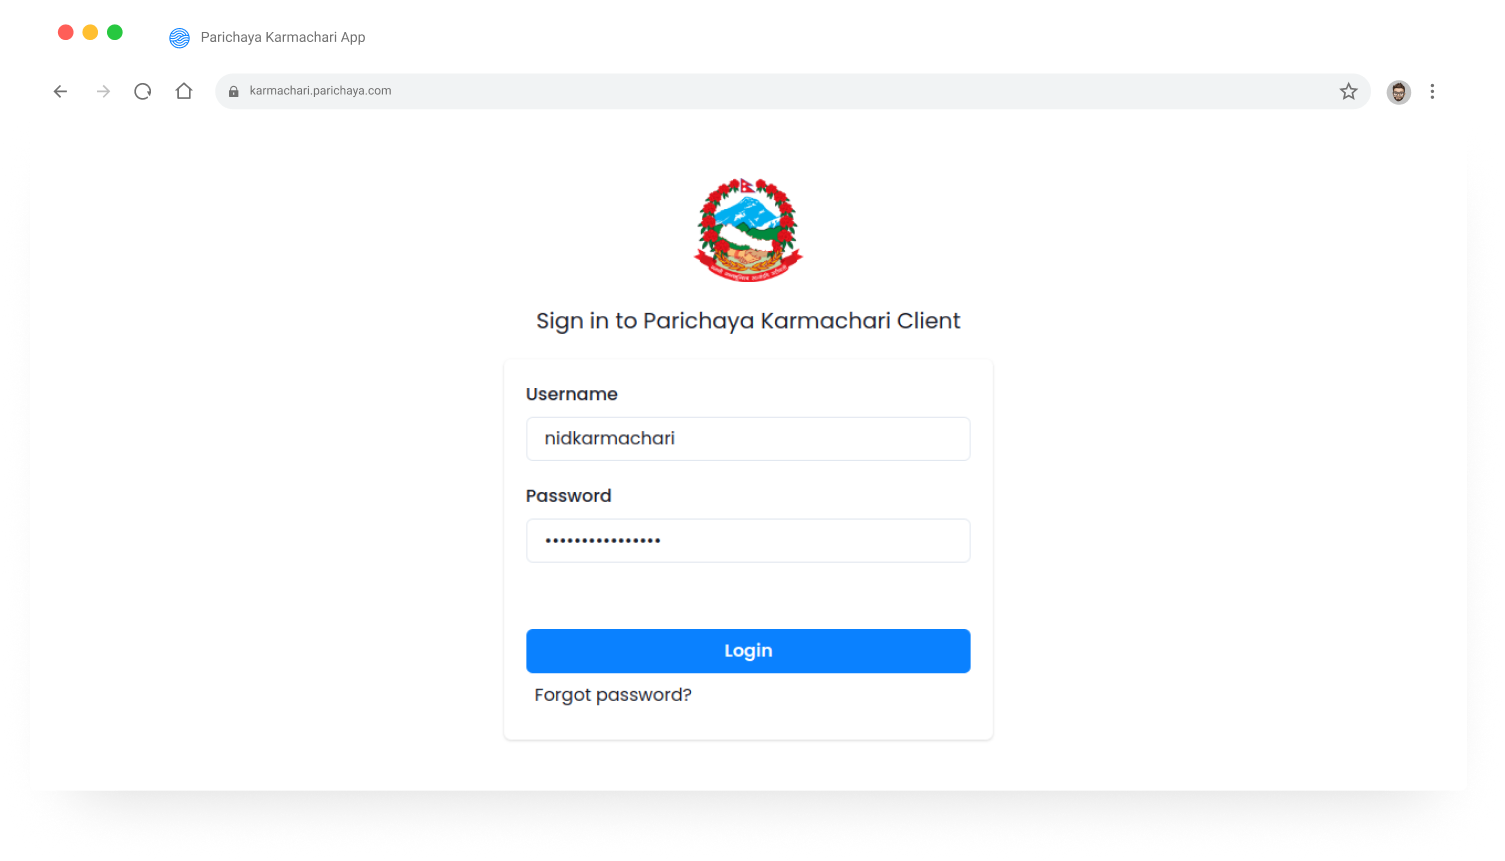
\includegraphics[width=0.6\linewidth]{images/results/web/FilledWebLogin.png}
        \caption[Filled Login]{Filled Login}
        \label{fig:FilledWebLogin.png}
        \end{figure}

   
    

     \begin{figure}[H]
        \centering
        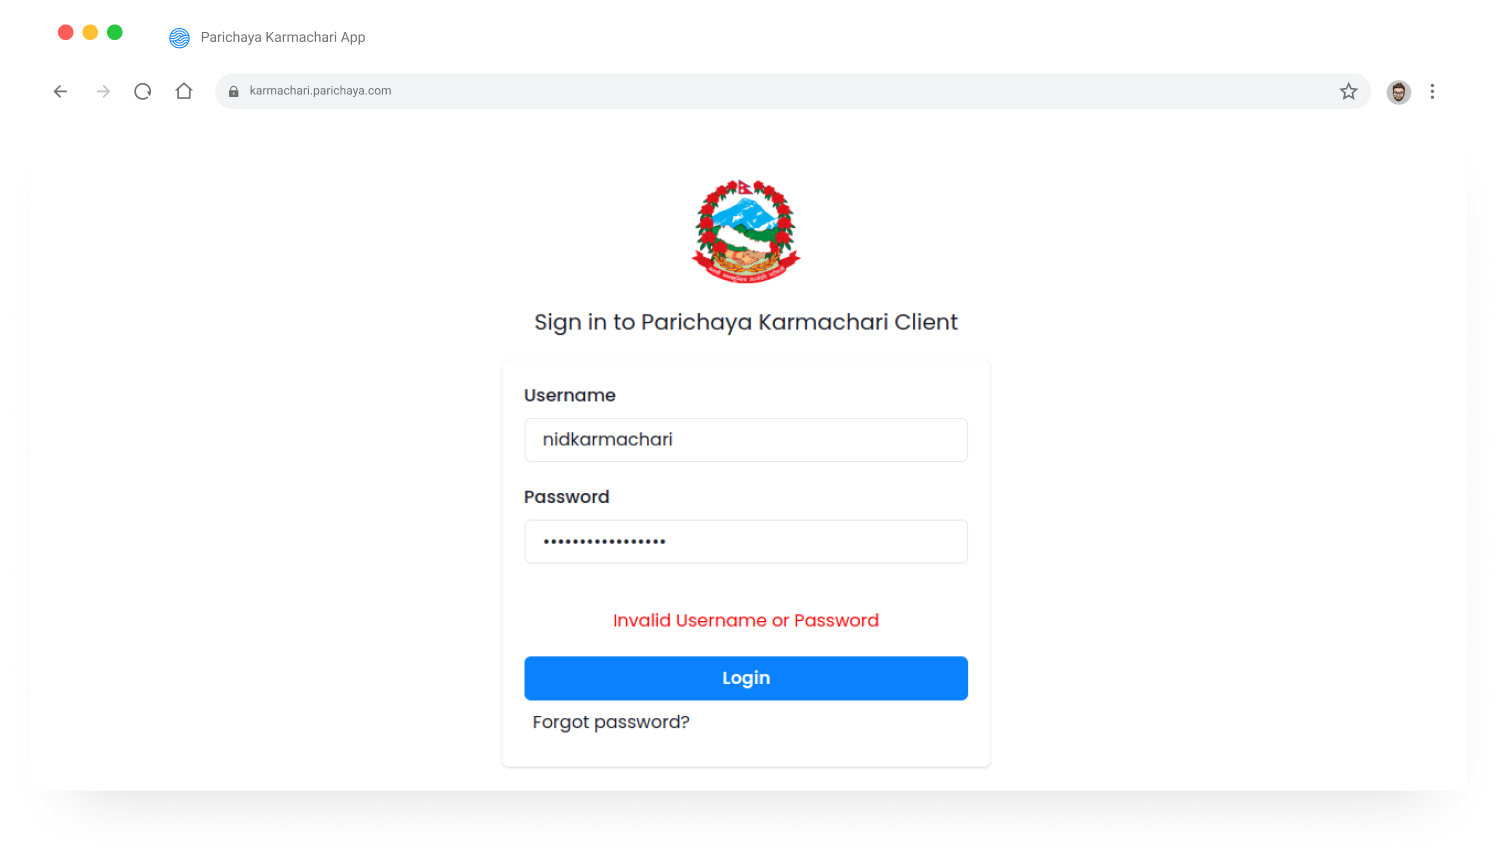
\includegraphics[width=0.6\linewidth]{images/results/web/WebLoginErrorPage.png}
        \caption[Login Error page ]{Login Error page}
        \label{fig:WebLoginErrorPage.png}
        \end{figure}
    Government Employee after logging in get to the home page. Here they can search for various identity documents like national identity card, citizenship card and driving license of any citizen based on their national identity number.In the left side of the homepage, there is vertical navigation bar which contains homepage, National identity card, Citizenship Card and Driving License.

        \begin{figure}[H]
        \centering
        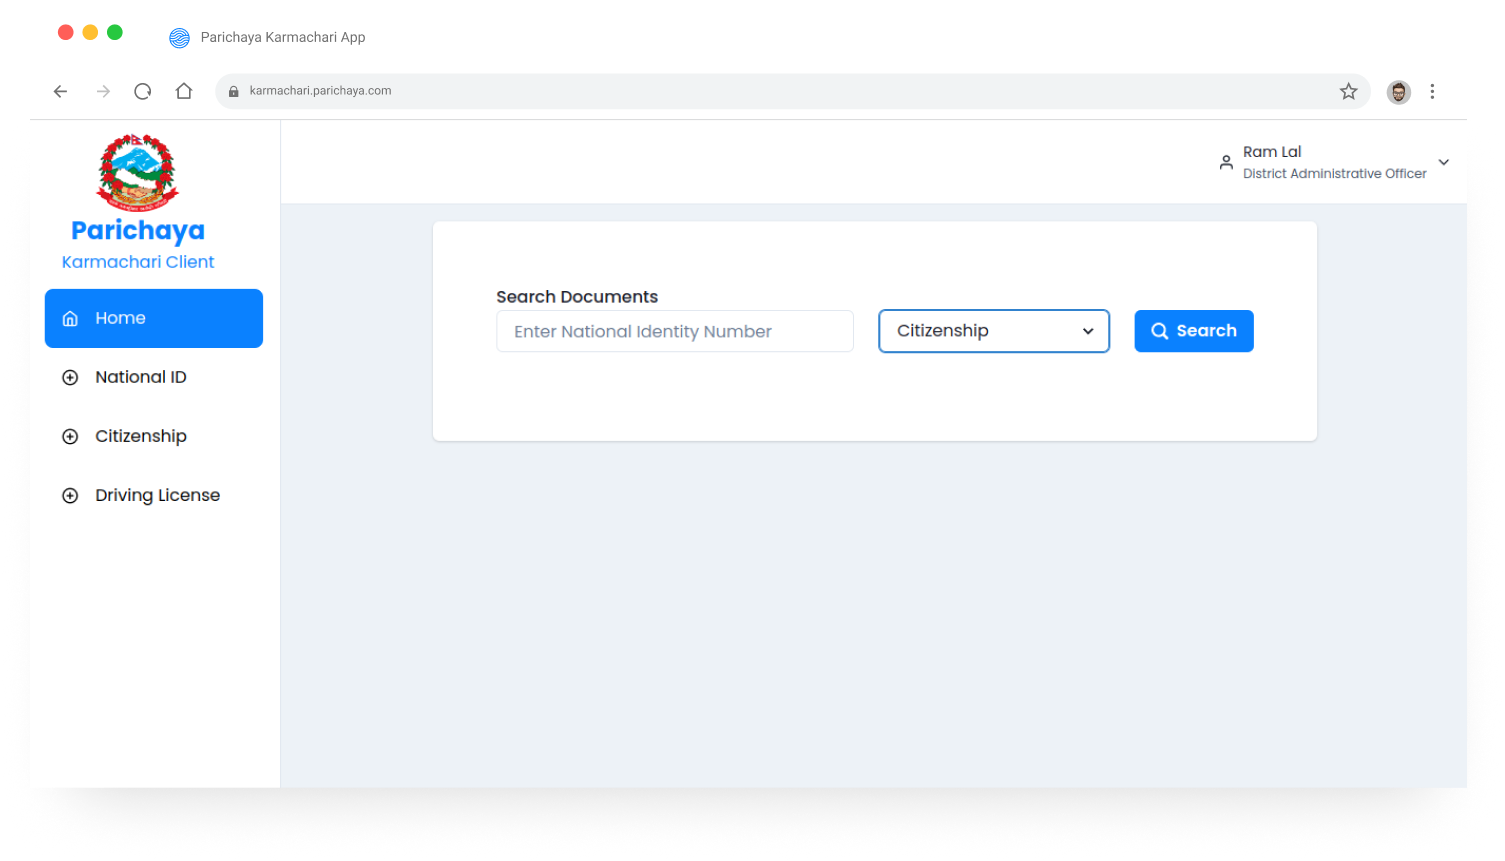
\includegraphics[width=0.8\linewidth]{images/results/web/WebHomePage.png}
      \caption[Home Page]{Home Page}
        \label{fig:WebHomePage.png}
        \end{figure}

           \begin{figure}[H]
        \centering
        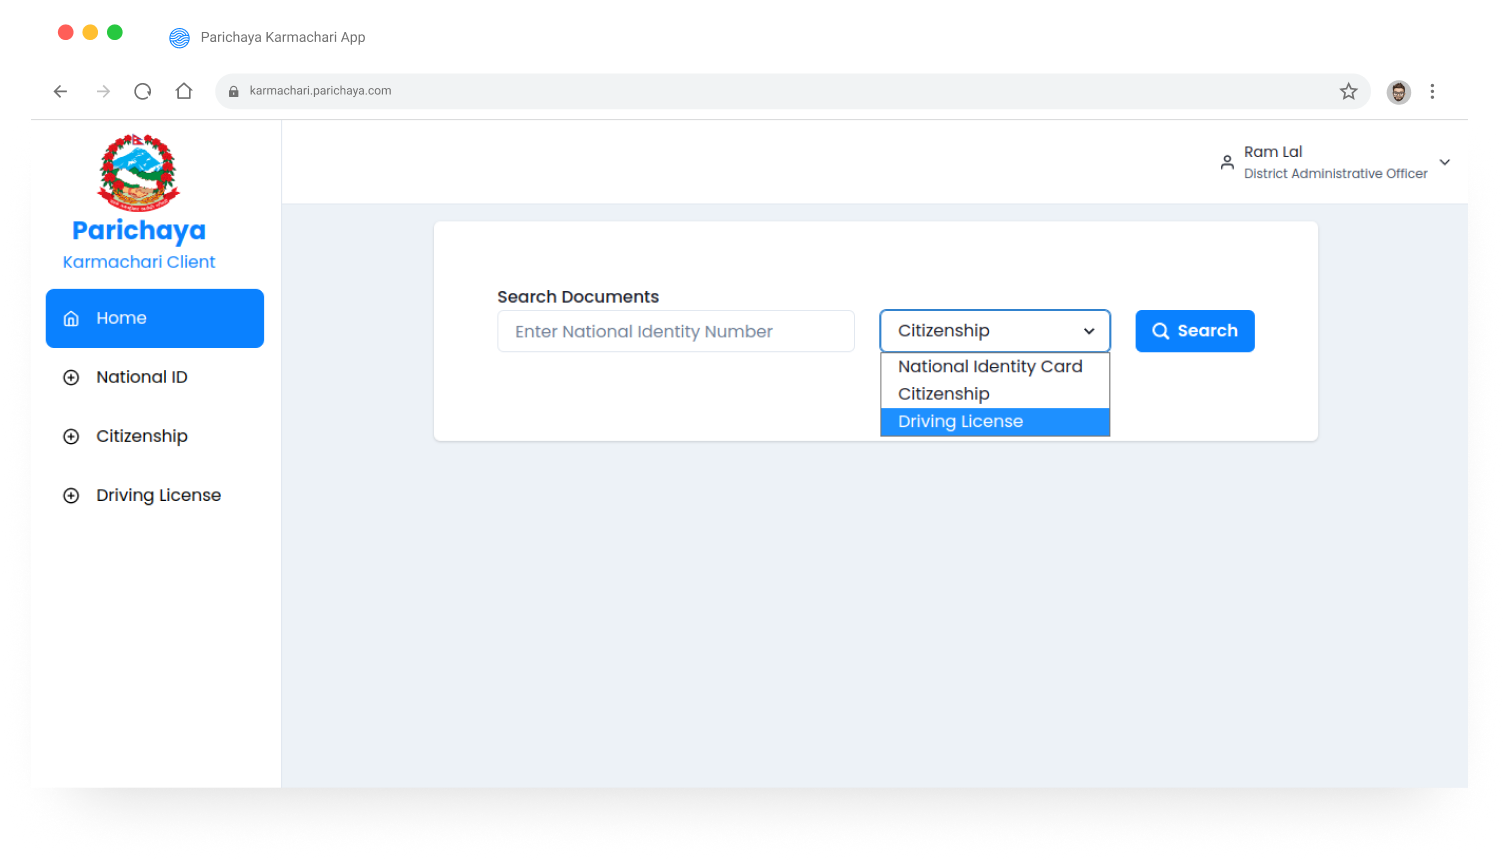
\includegraphics[width=0.8\linewidth]{images/results/web/WebHomePage2.png}
        \caption[Filled Home Page]{Filled Home Page}
        \label{fig:WebHomePage2.png}
        \end{figure}

           \begin{figure}[H]
        \centering
        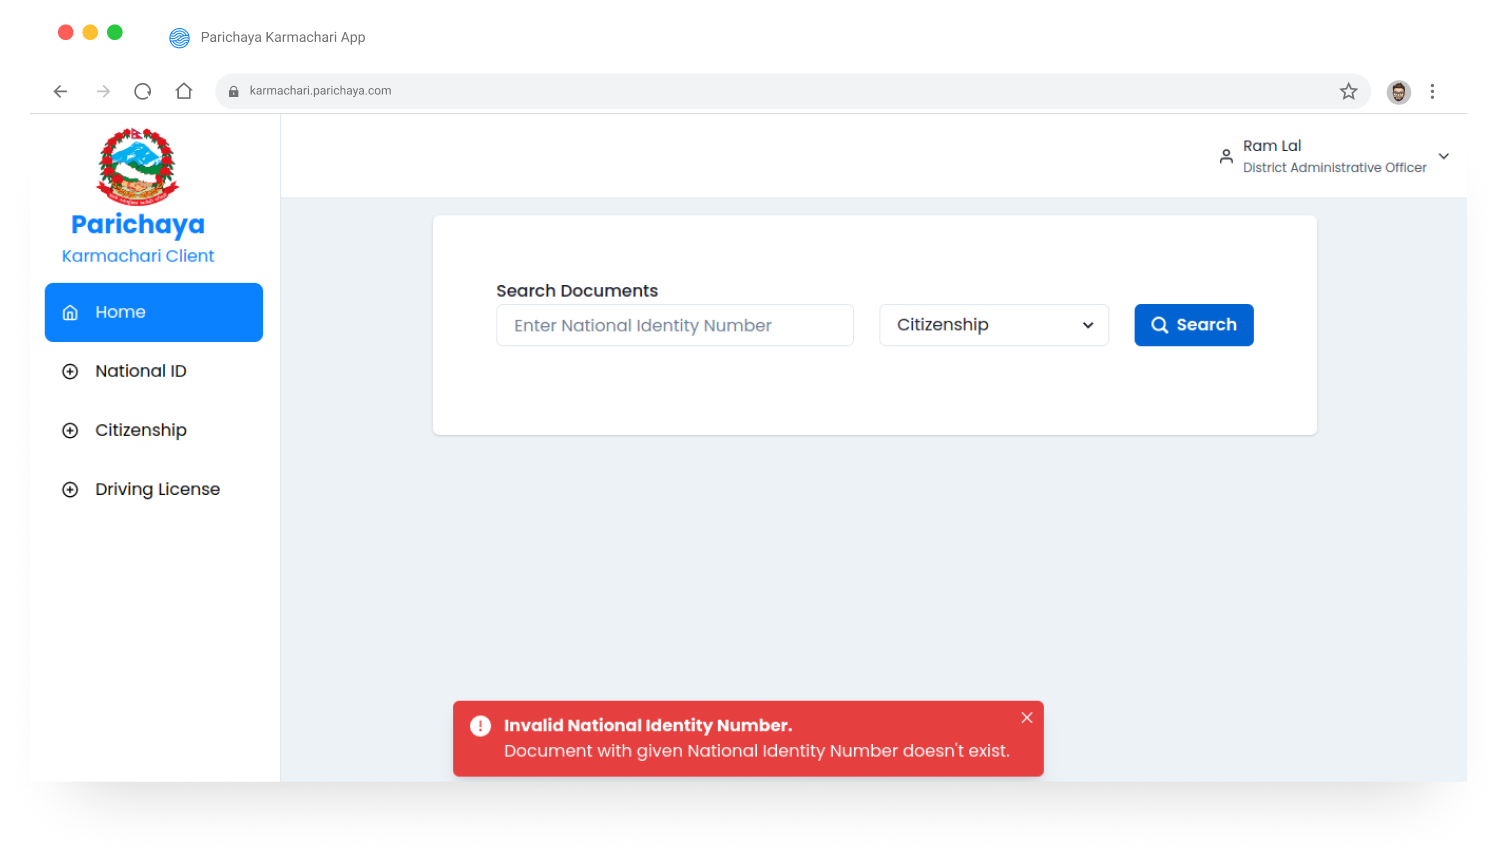
\includegraphics[width=0.8\linewidth]{images/results/web/WebHomeError.png}
        \caption[Home error Page ]{Home error Page }
        \label{fig:WebHomeError.png}
        \end{figure}


    By clicking on National ID in the vertical navbar, we go to National identity registration page where we can register NID card for citizens. 
   
        \begin{figure}[H]
        \centering
        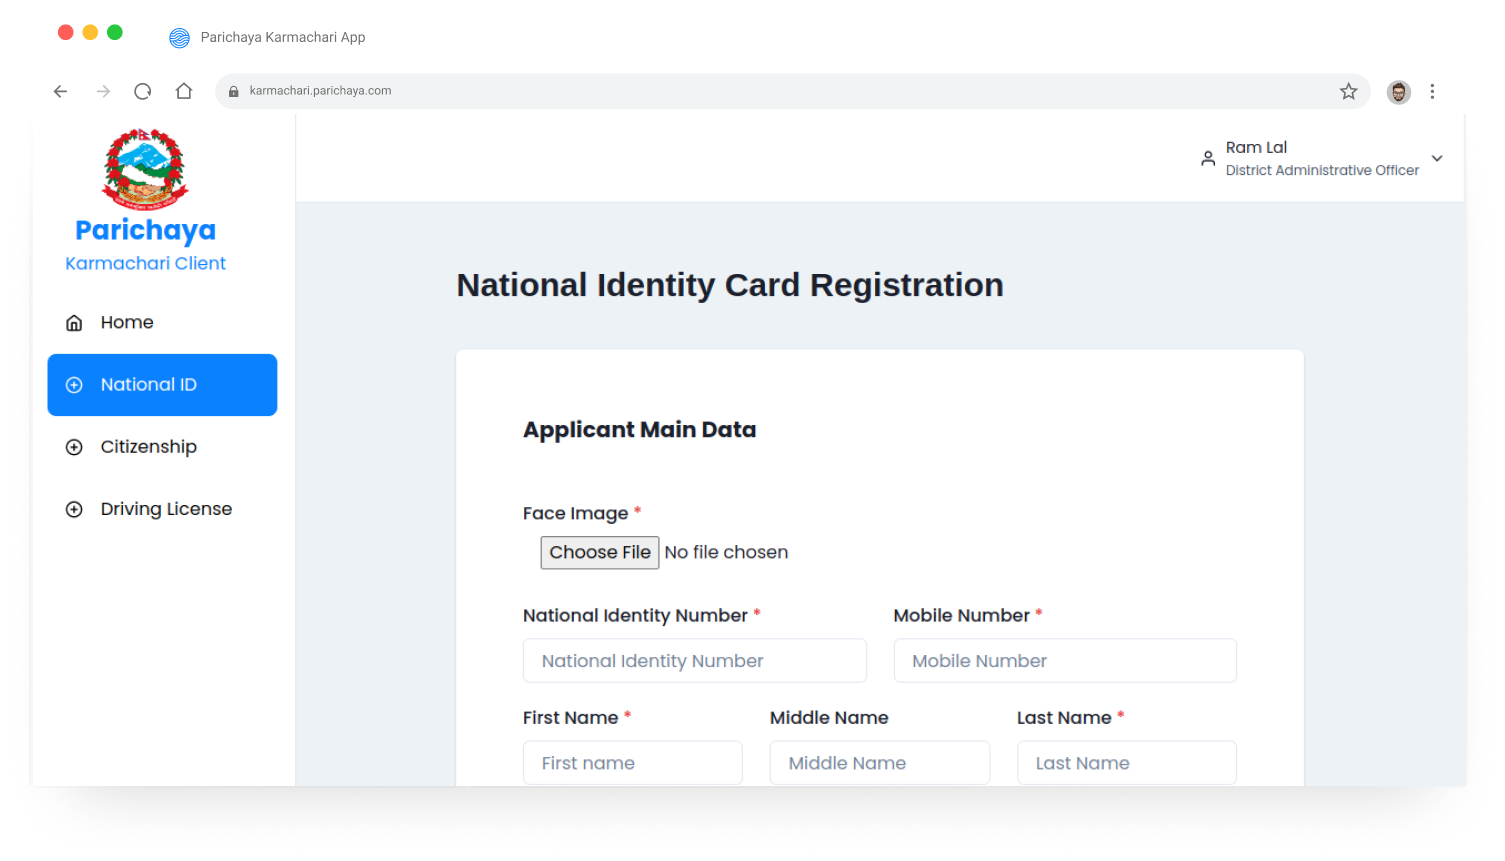
\includegraphics[width=0.8\linewidth]{images/results/web/WebNationalIDCardRegistration1.png}
        \caption[National ID Form]{National ID Form}
        \label{fig:WebNationalIDCardRegistration1.png}
        \end{figure}

           \begin{figure}[H]
        \centering
        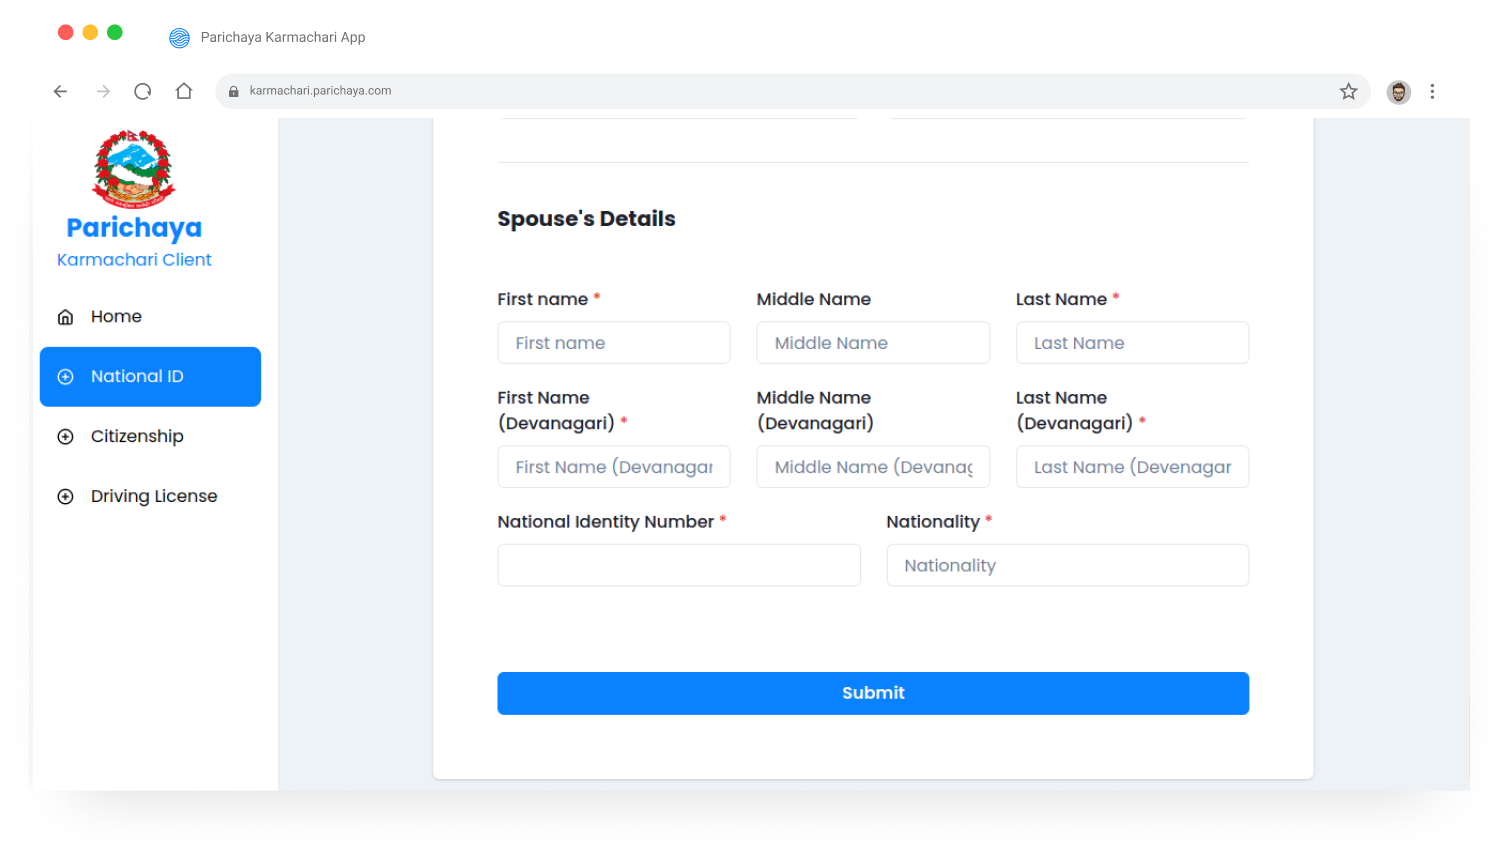
\includegraphics[width=0.8\linewidth]{images/results/web/WebNationalIDCardRegistration2.png}
        \caption[National ID Form]{National ID Form}
        \label{fig:WebNationalIDCardRegistration2.png}
        \end{figure}

    In this project, every identity documents is tied to National Identity Number. Therefore, before accessing any identity documents of a user, his National identity number has to be filled first. Then Government Employee can access other identity documents. They can make changes to the identity documents if needed as well. 


        \begin{figure}[H]
        \centering
        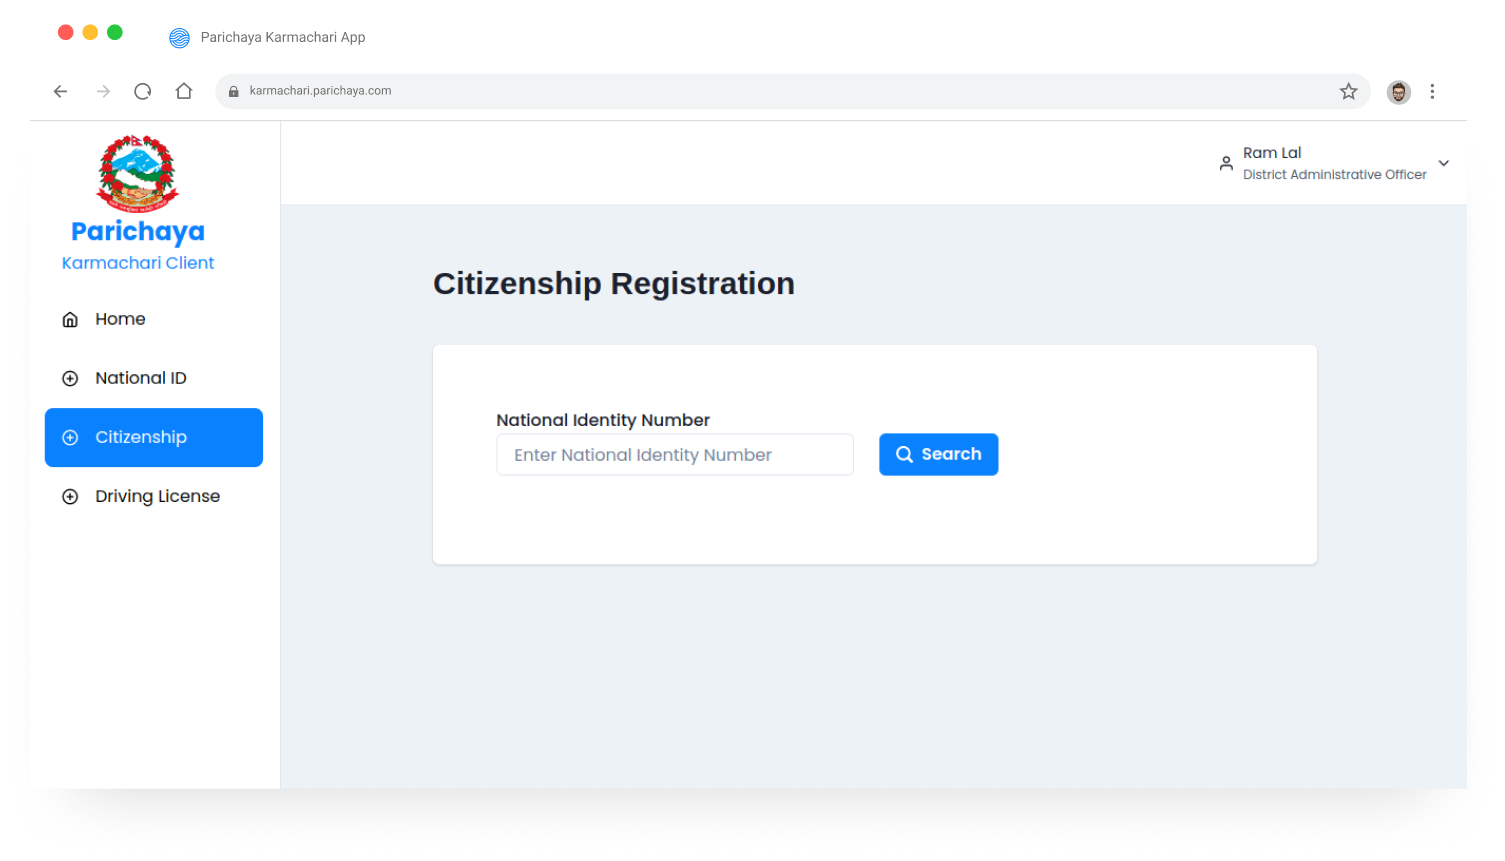
\includegraphics[width=0.8\linewidth]{images/results/web/WebCitizenshipRegistration1.png}
        \caption[Enter NIN]{Enter NIN}
        \label{fig:WebCitizenshipRegistration1.png}
        \end{figure}

           \begin{figure}[H]
        \centering
        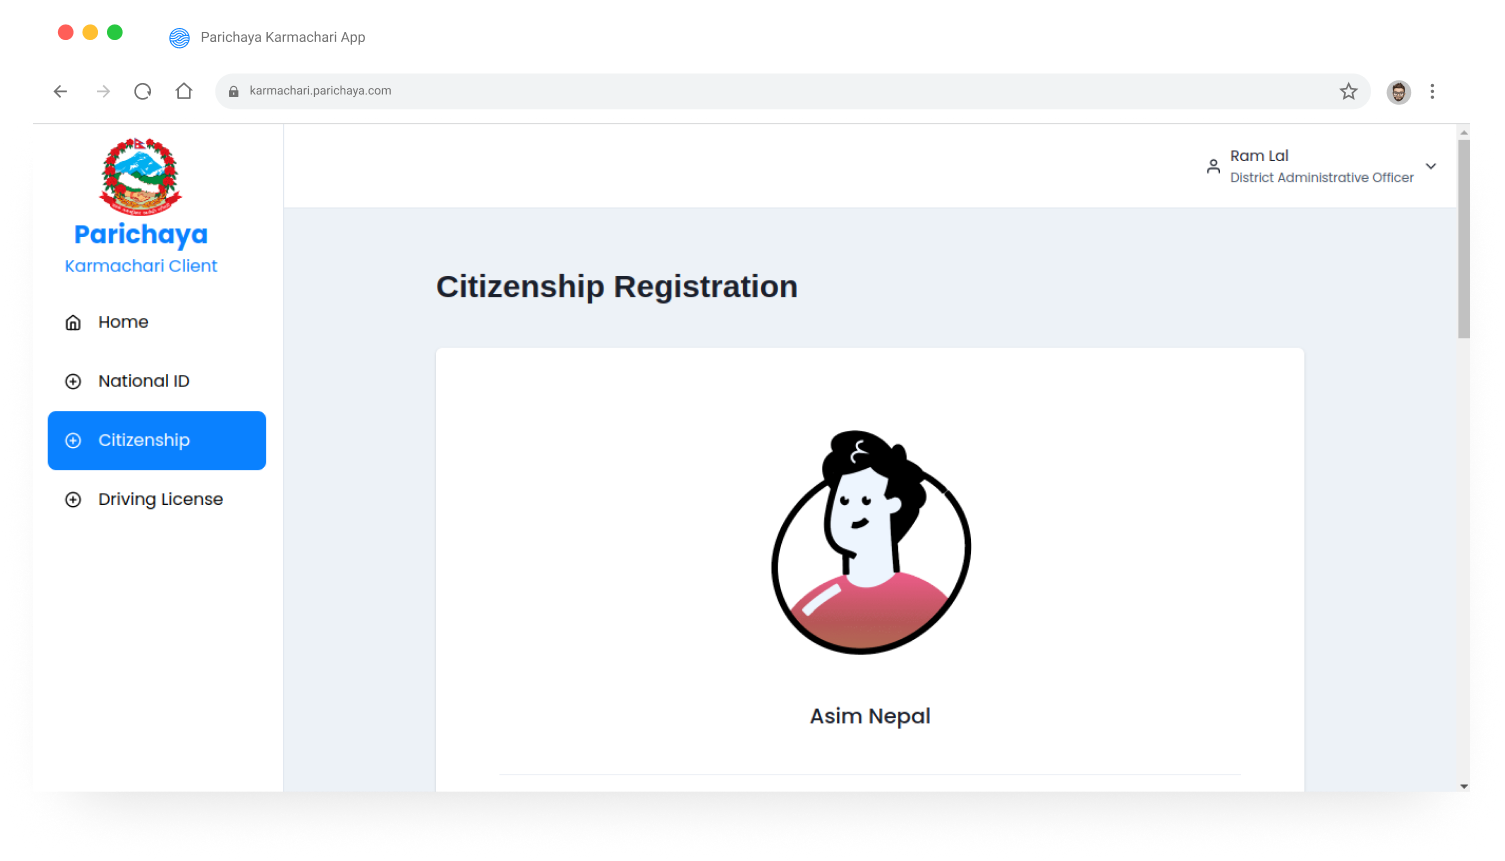
\includegraphics[width=0.8\linewidth]{images/results/web/WebCitizenshipRegistration2.png}
        \caption[Citizenship Card Form]{Citizenship Card Form}
        \label{fig:WebCitizenshipRegistration2.png}
        \end{figure}

          \begin{figure}[H]
        \centering
        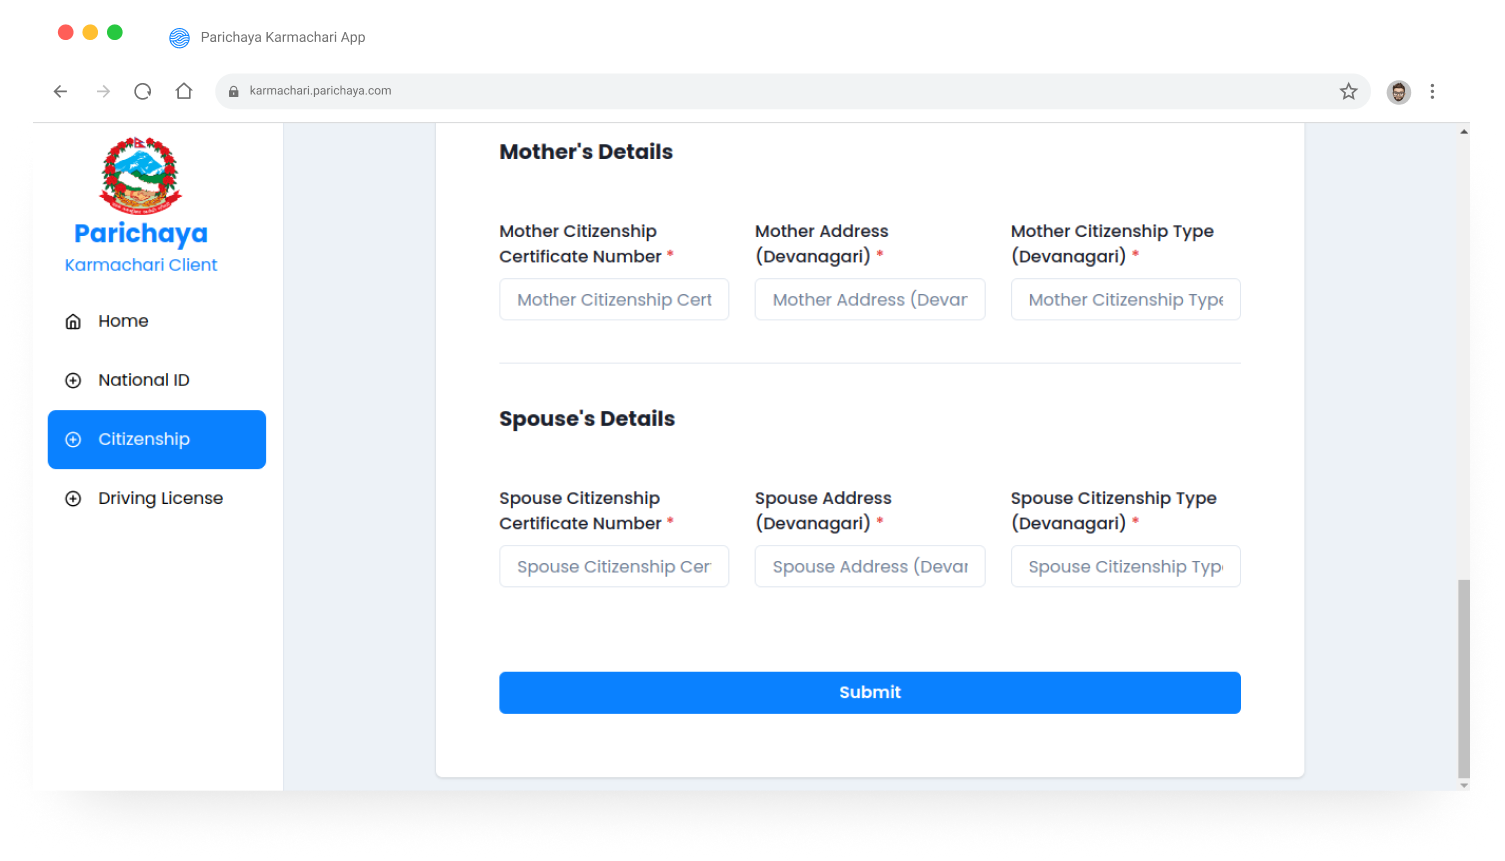
\includegraphics[width=0.8\linewidth]{images/results/web/WebCitizenshipRegistration3.png}
        \caption[Citizenship Card Form]{Citizenship Card Form}
        \label{fig:WebCitizenshipRegistration3.png}
        \end{figure}
    Similar to Citizenship card, to fill form or to access driving license or to make changes in the driving license,initially, National identity number of the citizen should be filled. 

        \begin{figure}[H]
        \centering
        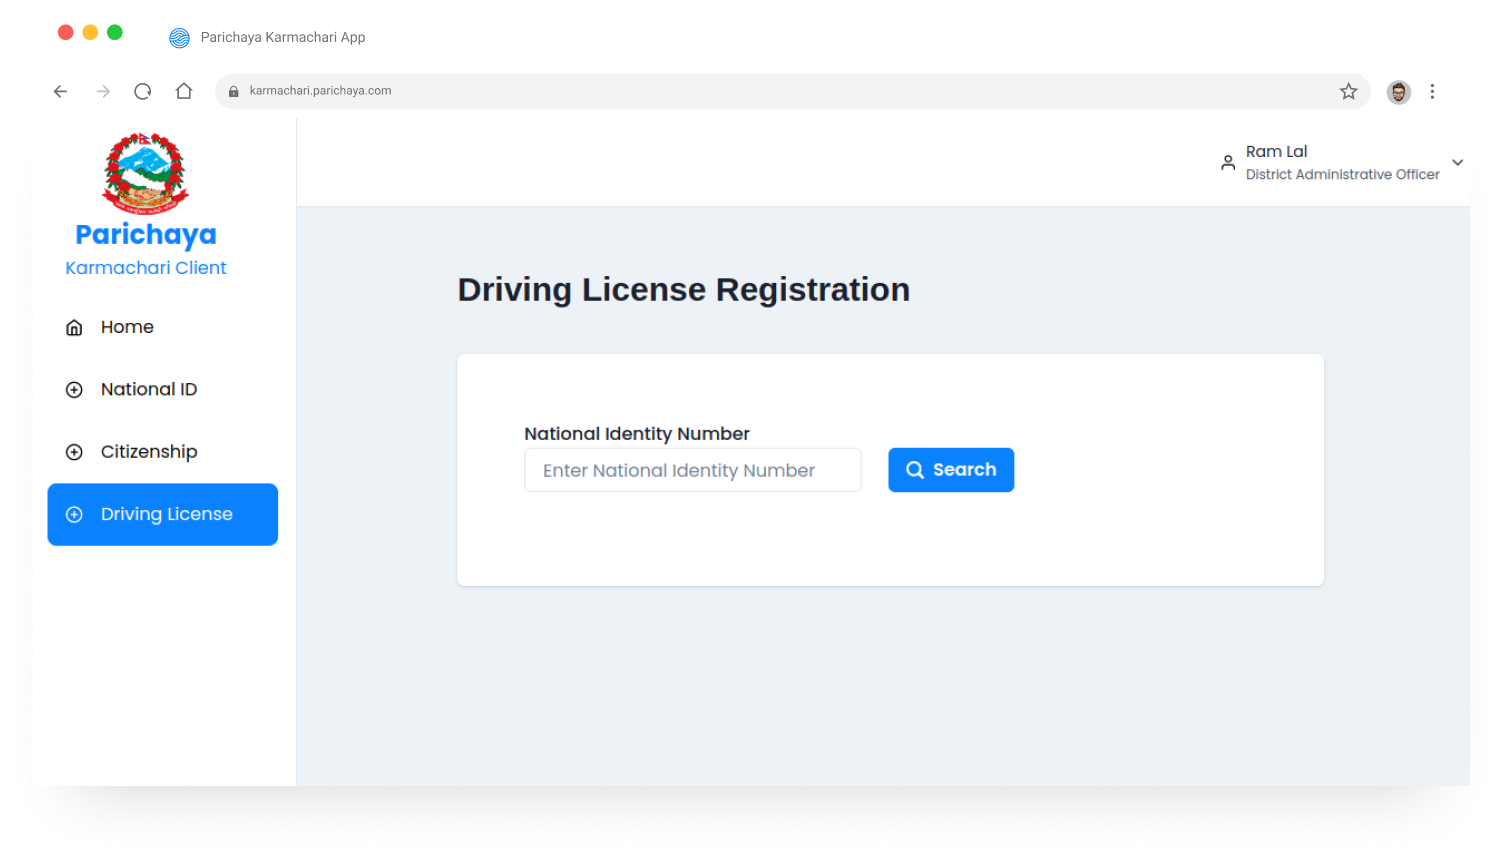
\includegraphics[width=0.8\linewidth]{images/results/web/WebDrivingLiceseRegistration1.png}
        \caption[Enter NIN]{Enter NIN}
        \label{fig:WebDrivingLiceseRegistration1.png}
        \end{figure}
           \begin{figure}[H]
        \centering
        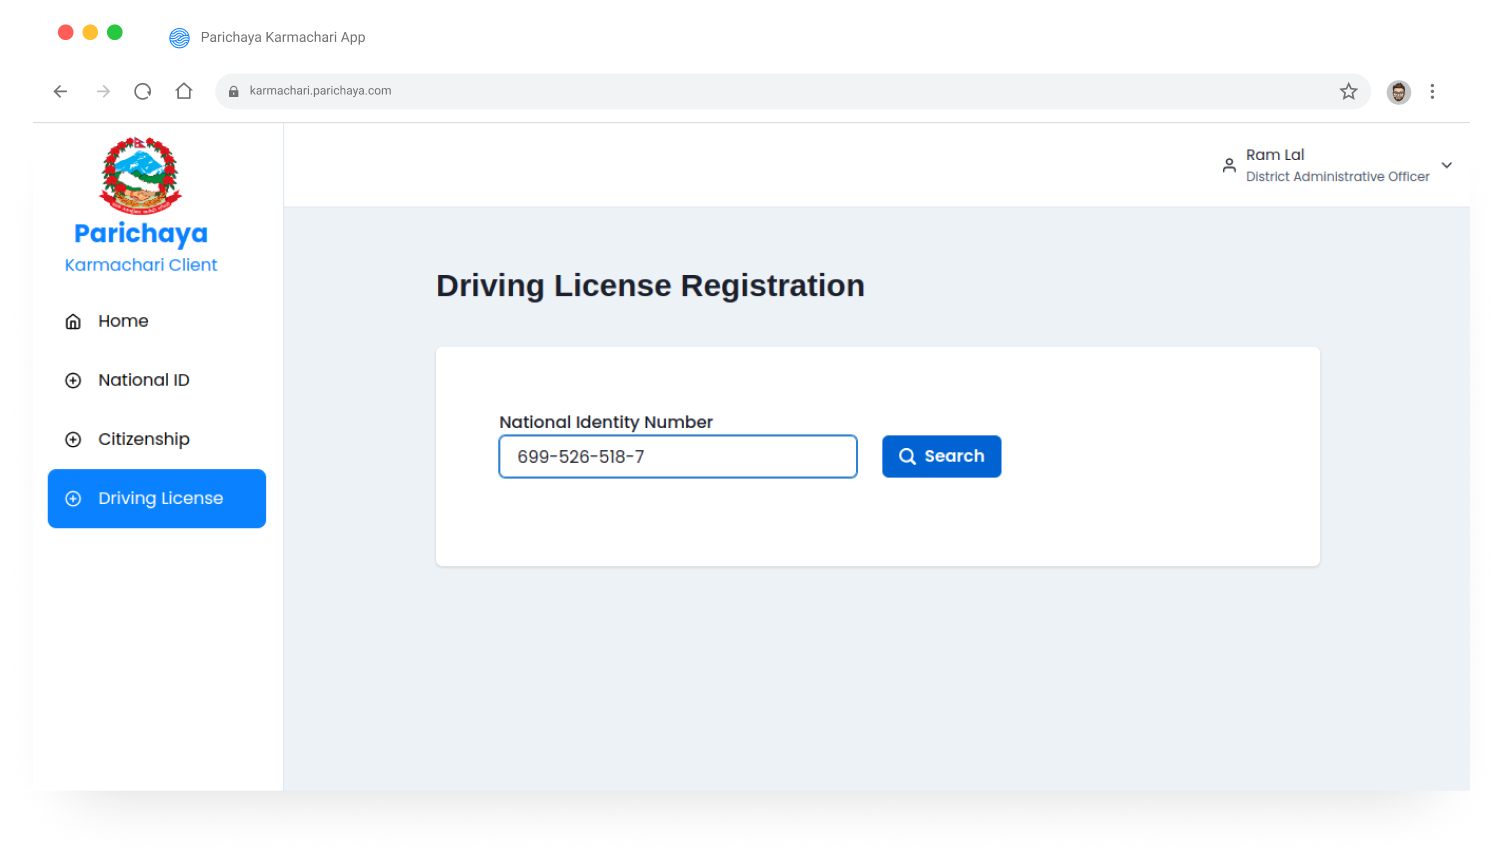
\includegraphics[width=0.8\linewidth]{images/results/web/WebDrivingLicenseRegistration2.png}
        \caption[Driving License Form]{Driving License Form}
        \label{fig:WebDrivingLicenseRegistration2.png}
        \end{figure}


        \begin{figure}[H]
        \centering
        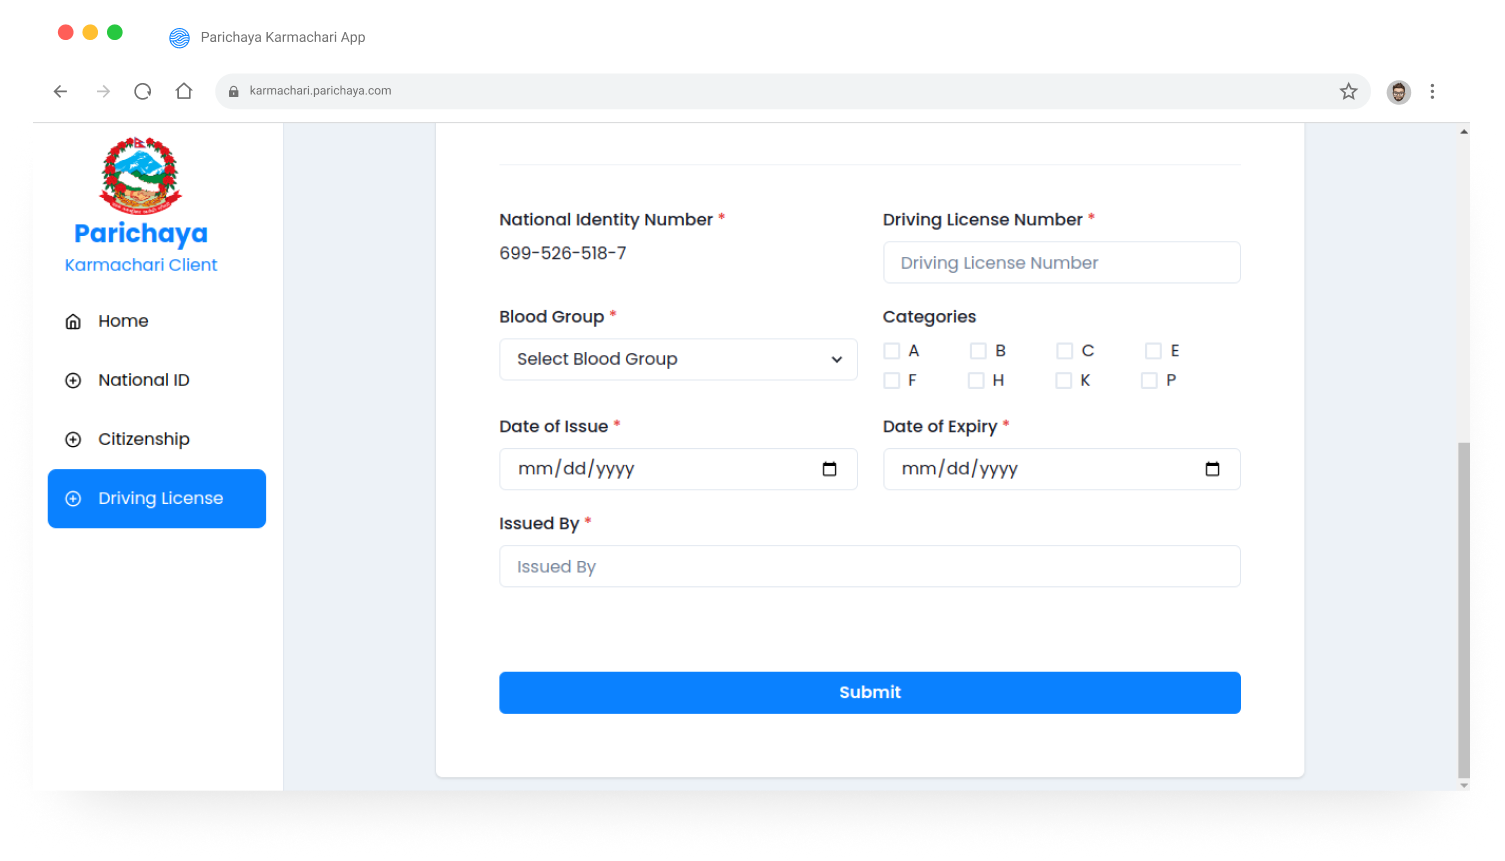
\includegraphics[width=0.8\linewidth]{images/results/web/WebDrivingLicenseRegistration3.png}
        \caption[Driving License Form]{Driving License Form}
        \label{fig:WebDrivingLicenseRegistration3.png}
        \end{figure}
        
    \subsection{Sharing Details to Third Party Web Client}
        User can directly fill form or share identity document details to third party applications like banks or governmental organization through Parichaya with a touch of a button.     
   
        \begin{figure}[H]
        \centering
        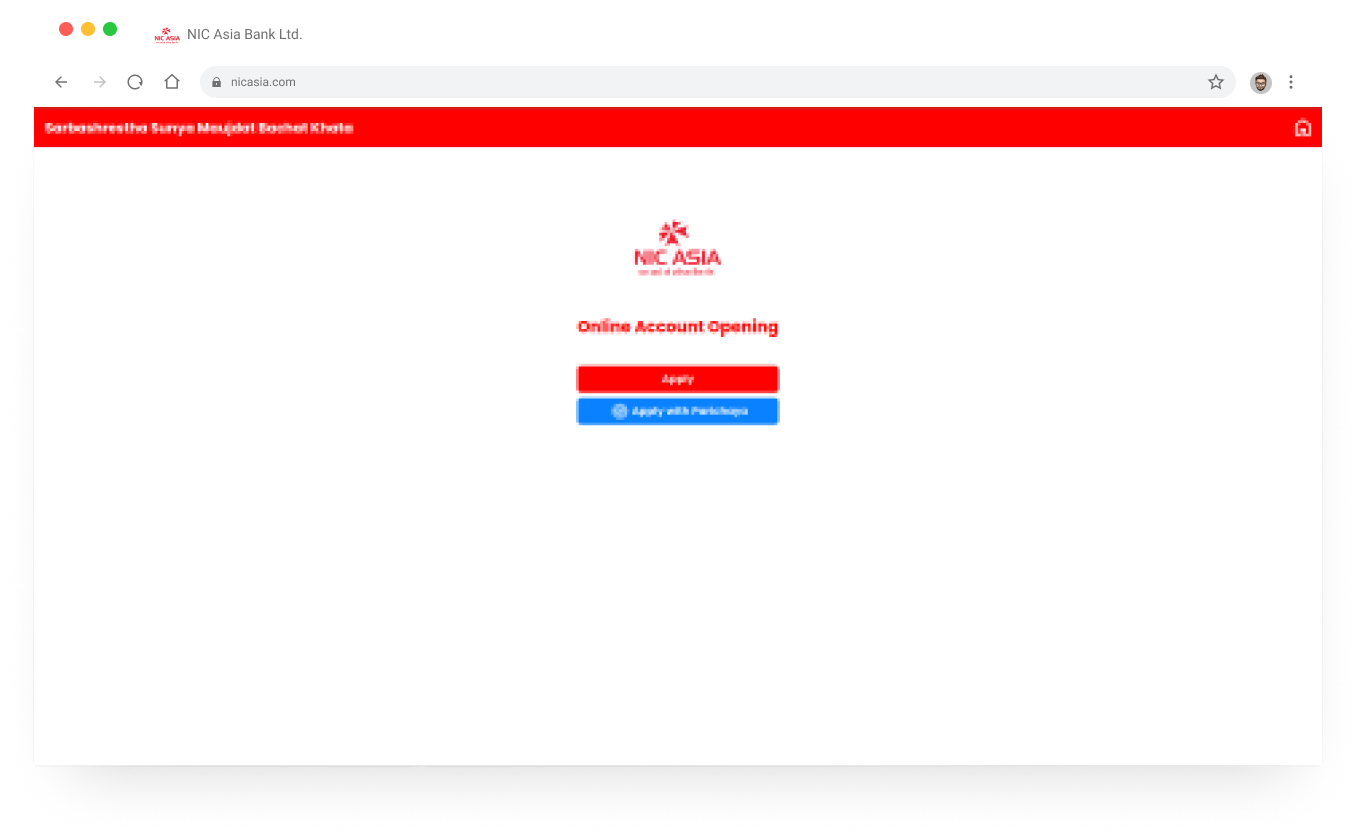
\includegraphics[width=0.8\linewidth]{images/results/web/NICApply.png}
        \caption[Nic Asia Apply]{Nic Asia Apply}
        \label{fig:NICApply.png}
        \end{figure}
        % \newpage
    After clicking the button, a QR code is generated along with the required data fields. Users can scan the QR code using Parichaya mobile app to view the requester's details along with the requested data fields. 
        \begin{figure}[H]
        \centering
        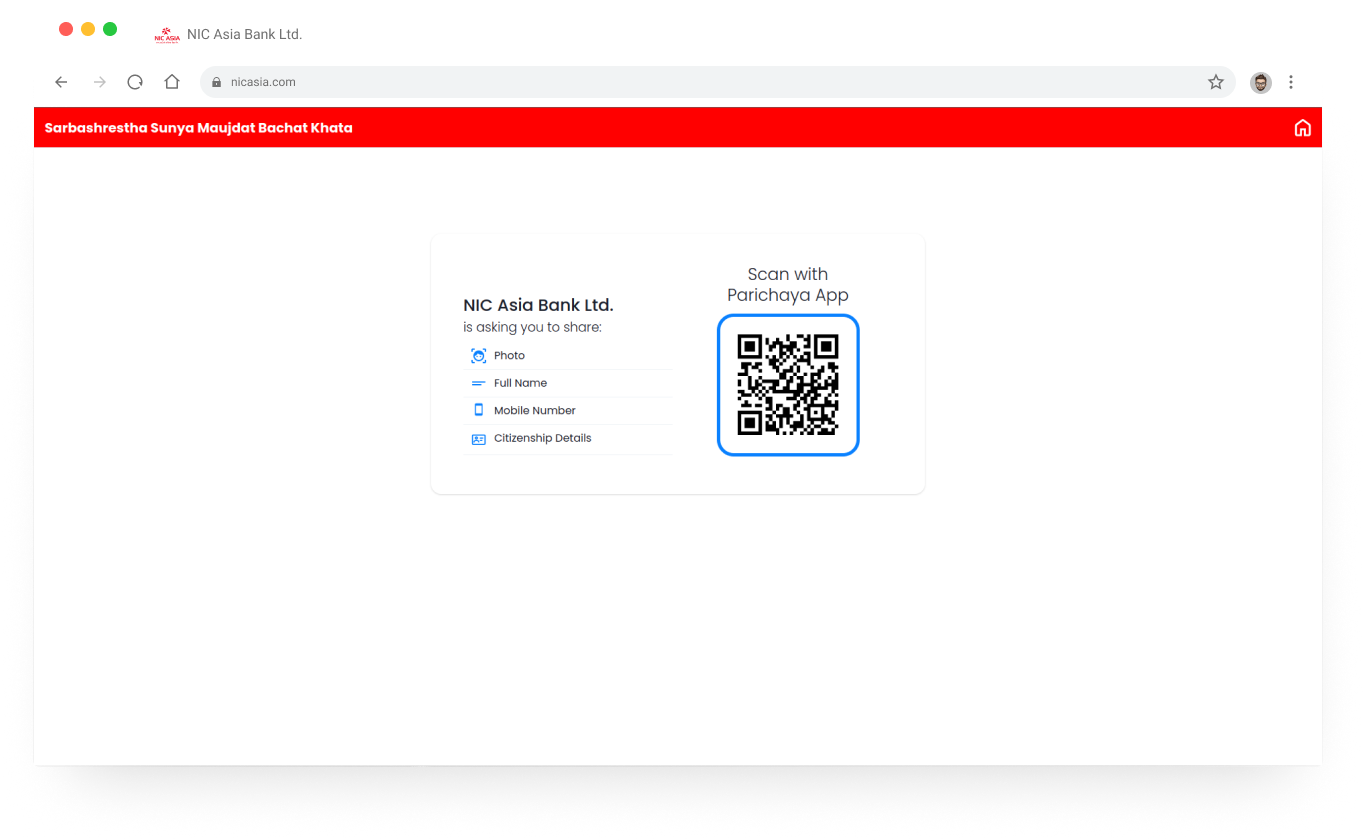
\includegraphics[width=0.8\linewidth]{images/results/web/NICQR.png}
        \caption[Nic Asia QR]{Nic Asia QR}
        \label{fig:NICQR.png}
        \end{figure}
         \begin{figure}[H]
        \centering
        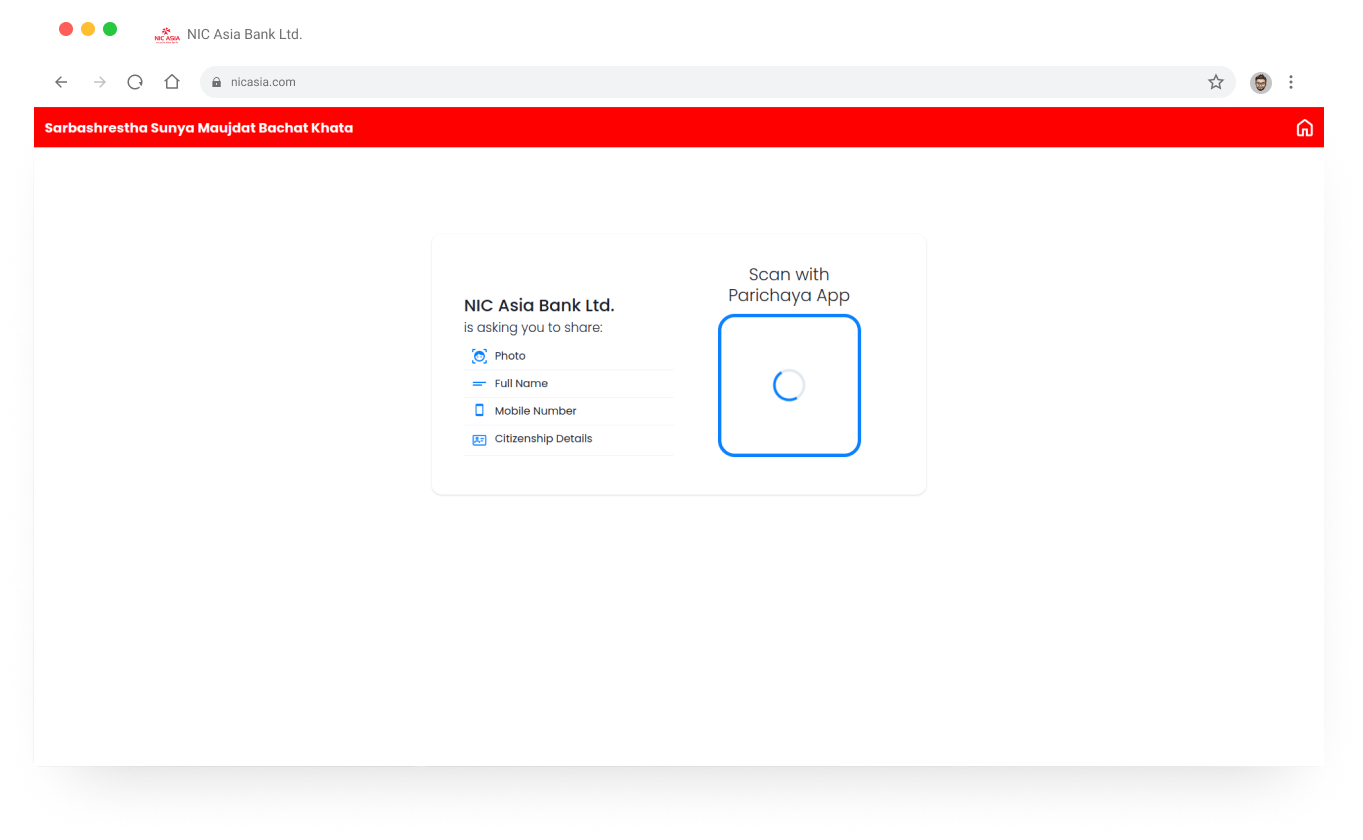
\includegraphics[width=0.8\linewidth]{images/results/web/NICLoading.png}
        \caption[Nic Asia Loading]{Nic Asia Loading}
        \label{fig:NICLoading.png}
        \end{figure}
        % \newpage
        If the user approves the data request, the requested data are shown. Else, a rejection message is showned to the user.  
         \begin{figure}[H]
        \centering
        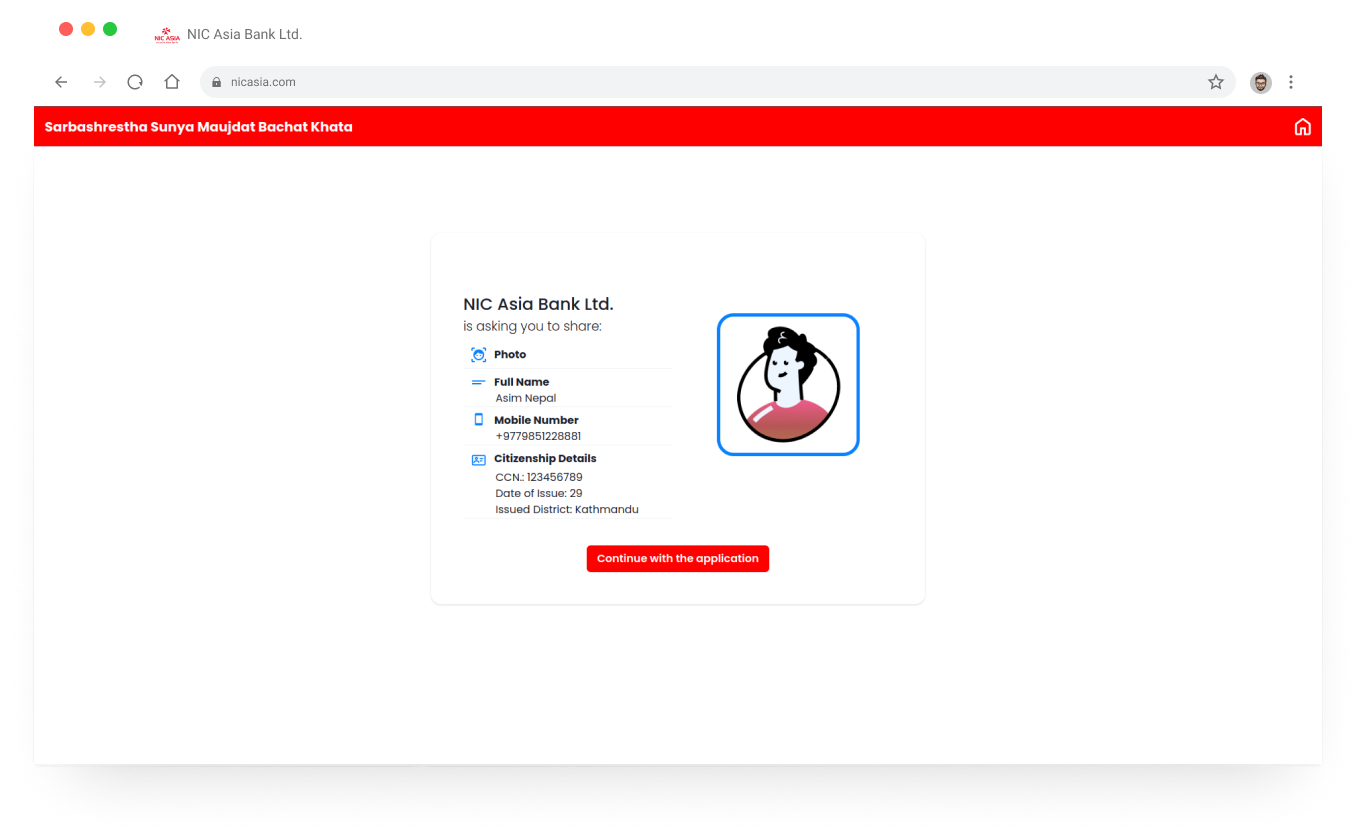
\includegraphics[width=0.8\linewidth]{images/results/web/NICDetails.png}
        \caption[Nic Asia Details]{Nic Asia Details}
        \label{fig:NICDetails.png}
        \end{figure}
        \begin{figure}[H]
        \centering
        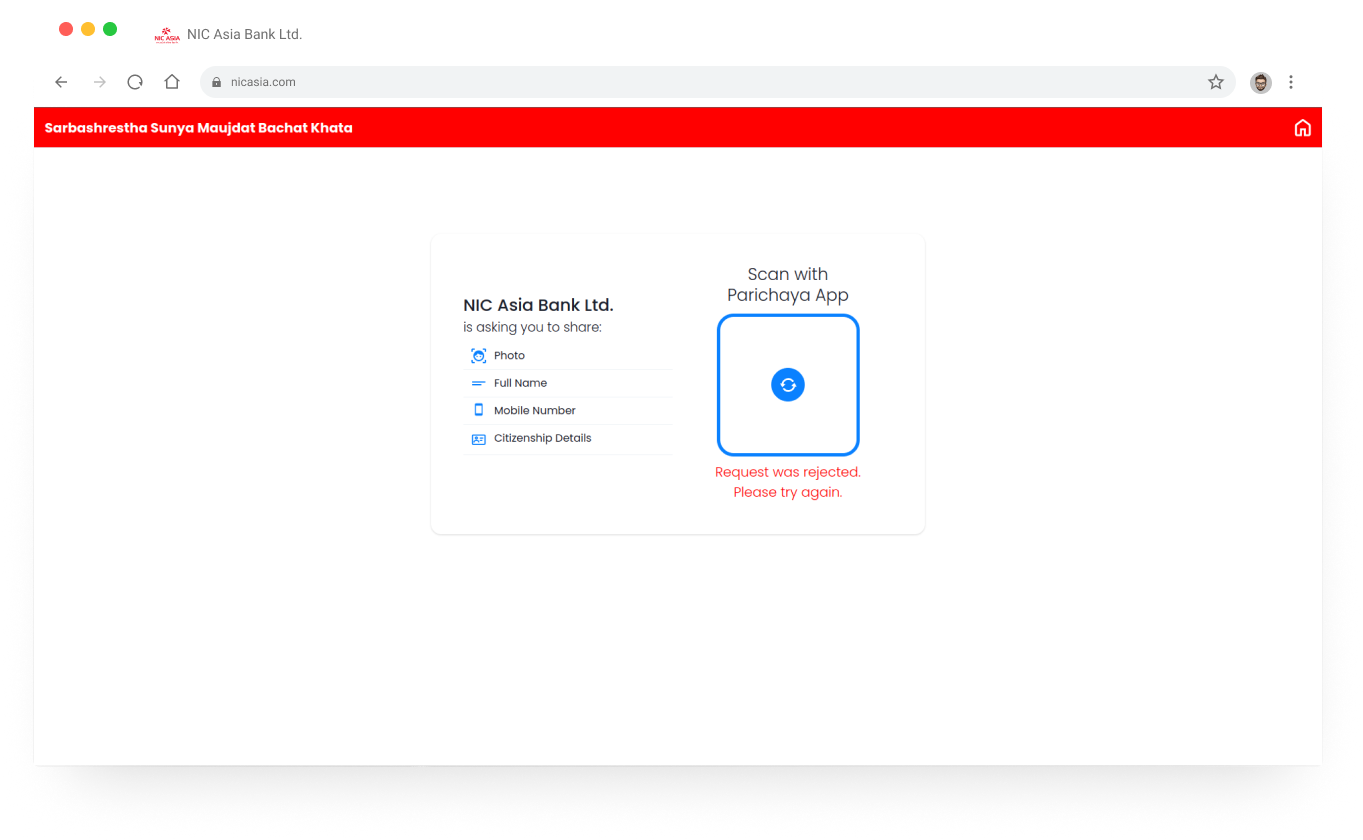
\includegraphics[width=0.8\linewidth]{images/results/web/NICRejected.png}
        \caption[Nic Asia Rejected]{Nic Asia Rejected}
        \label{fig:NICRejected.png}
        \end{figure}
        


\section{Discussion}
The report highlights the need for an upgraded digital authentication system in Nepal, as the current process heavily relies on physical documents and centralized storage, leading to inefficiencies and security risks. To address these challenges, the proposal suggests implementing a blockchain-based digital identity system called "Parichaya" using Hyperledger Fabric technology. The system aims to provide secure and tamper-proof storage of citizens' documents, improve government service delivery, and enhance convenience for users. The use of blockchain technology can prevent identity fraud, ensure data integrity, and enable faster verification processes. While the system presents numerous benefits, there are potential limitations to consider, such as the reliance on government officials' authentication and the need for data encryption to enhance security. However, the proposal also discusses opportunities for future research and application, including integration into other sectors like healthcare, supply chain management, and institutional account creation processes. Overall, the report highlights the importance of upgrading Nepal's authentication system and the potential of blockchain technology to address the identified challenges.

      


